\documentclass[10pt, a4paper]{article}
\usepackage[slovene]{babel}
\usepackage[T1]{fontenc}
\usepackage[utf8]{inputenc}
\usepackage{lmodern}
\usepackage{amsmath}
\usepackage{amsthm}
\usepackage{amssymb}
\usepackage{parskip}
\usepackage{pgfplots}
\pgfplotsset{compat=1.8}
\usepackage{comment}
\usepackage{graphicx}
\usepackage{booktabs}
\usepackage{array}
\usepackage{float}
%\usepackage{mdframed}
%\usepackage{thmbox}

%%%%%%%%%%%%%%%%%%%%%%%%%%%%%%%%%%%%%%%%%%%%%%%%%%%%%%%%%%%%%%%%%%%%%%

\usepackage[top=105pt, bottom=75pt, left=75pt, right=75pt]{geometry}
\setlength{\headsep}{15pt}
\setlength{\footskip}{45pt}

\usepackage{xcolor}
\usepackage{lipsum}

\usepackage{ifthen}
\usepackage{tikz}
\usetikzlibrary{calc}
\usetikzlibrary{cd}
\usetikzlibrary{babel}
\usepackage[all,cmtip]{xy}


%%%%%%%%%%%%%%%%%%%%%%%%%%%%%%%%%%%%%%%%%%%%%%%%%%%%%%%%%%%%%
\usepackage{tcolorbox}
\tcbuselibrary{skins, breakable}

\usepackage{multirow, makecell}
\usepackage{siunitx}

%%%%%%%%%%%%%%%%%%%%%%%%%%%%%%
%%% with separate title
\xdefinecolor{thmTopColor}{RGB}{102, 102, 238}
\xdefinecolor{thmBackColor}{RGB}{245, 245, 255}

%%%%%%%%%%%%%%%%%%%%%%%%%%%%%%%%%%%%%%%%%%%%%%%%%%%%%%%%%%%%%%%%%%%%%%%%



\newtheorem{izr}{Izrek}[section]

\newenvironment{thmbox}[1]{%
  \tcolorbox[%
  empty,
  parbox=false,
  noparskip,
  enhanced,
  breakable,
  sharp corners,
  boxrule=-1pt,
  left=2ex,
  right=0ex,
  top=0ex,
  boxsep=1ex,
  before skip=2.5ex plus 2pt,
  after skip=2.5ex plus 2pt,
  colback=thmBackColor,
  colframe=white,
  coltitle=black,
  colbacktitle=thmBackColor,
  fonttitle=\bfseries,
  title=#1,
  titlerule=1pt,
  titlerule style=thmTopColor,
  overlay unbroken and last={%
    \draw[color=thmTopColor, line width=1.25pt]
    ($(frame.north west)+(.5em, -4.1ex)$)
    -- ($(frame.south west)+(.5em, 1ex)$) -- ++(2em, 0);
  }]
}{\endtcolorbox}

\newenvironment{izrek}[1][]{% before
  \refstepcounter{izr}%
  \ifthenelse{\equal{#1}{}}{%
    \begin{thmbox}{Izrek \theizr.}\itshape\hspace{-.75ex}%
  }{%
    \begin{thmbox}{Izrek \theizr%
        \hspace{.75ex}(\textnormal{#1}).}\itshape\hspace{-.75ex}
    }}
  {\end{thmbox}
}

{\theoremstyle{plain}
\newtheorem{posledica}[izr]{Posledica}
\newtheorem{trditev}[izr]{Trditev}

}

{\theoremstyle{definition}
\newtheorem{defi}{Definicija}[section]
\newtheorem{aksiom}{Aksiom}[section]
}

\newenvironment{noticeB}{%
  \tcolorbox[%
  notitle,
  empty,
  enhanced,  % delete the edge of the bottom page for a broken box
  breakable,
  coltext=black,
  colback=white, 
  fontupper=\rmfamily,
  parbox=false,
  noparskip,
  sharp corners,
  boxrule=-1pt,  % width of the box' edges
  frame hidden,
  left=7pt,  % inner space from text to the left edge
  right=7pt,
  top=5pt,
  bottom=5pt,
  % boxsep=0pt,
  before skip=2.5ex plus 2pt,
  after skip=2.5ex plus 2pt,
  borderline west = {1.5pt}{-0.1pt}{blue!30!black}, % second argument = offset
  overlay unbroken and last={%
    \draw[color=black, line width=1.25pt]
    ($(frame.south west)+(1.pt, -0.1pt)$) -- ++(2em, 0);
  }
  ]}
{\endtcolorbox}

\newenvironment{definicija}{\begin{defi}\begin{noticeB}}{%
    \end{noticeB}\end{defi}}

{\theoremstyle{remark}
\newtheorem*{opomba}{Opomba}
}

\newtheorem{zgled}{Zgled}[section]
\tcolorboxenvironment{zgled}{%
  enhanced jigsaw,
  boxrule=-1pt,
  colframe=gray!15,
  %borderline west={2pt}{0pt}{black},  % second argument is the offset
  interior hidden,
  sharp corners,
  breakable,
  before skip=2.5ex plus 2pt,
  after skip=2.5ex plus 2pt
}

%%%%%%%%%%%%%%%%%%%%%%%%%%%%%%%%%%%%%%%%%%%%%%%%%%%%%%%%%%%%%%%%%%%%%%%%
\newtheorem{lema}[izr]{Lema}
\tcolorboxenvironment{lema}{%
  enhanced jigsaw,
  boxrule=-1pt,
  colframe=white,
  borderline west={2pt}{0pt}{orange},  % second argument is the offset
  interior hidden,
  breakable,
  before skip=2.5ex plus 2pt,
  after skip=2.5ex plus 2pt
}

%%%%%%%%%%%%%%%%%%%%%%%%%%%%%%%%%%%%%%%%%%%%%%%%%%%%%%%%%%%%%%%%%%
\newenvironment{noticeC}{%
  \tcolorbox[%
  notitle,
  empty,
  enhanced,  % delete the edge of the bottom page for a broken box
  breakable,
  coltext=black, 
  fontupper=\rmfamily,
  parbox=false,
  noparskip,
  sharp corners,
  boxrule=-1pt,  % width of the box' edges
  frame hidden,
  left=7pt,  % inner space from text to the left edge
  right=7pt,
  top=5pt,
  bottom=5pt,
  % boxsep=0pt,
  before skip=2.5ex plus 2pt,
  after skip=2.5ex plus 2pt,
  %borderline west = {1.5pt}{-0.1pt}{gray}, % second argument = offset
  overlay unbroken and last={%
    %\draw[color=gray, line width=1.25pt]
    %($(frame.west)$);
    %\draw[color=gray, line width=1.25pt]
    %($(frame.east)$);
  },
  ]}
{\endtcolorbox}

\newenvironment{dokaz}%
  {\begin{noticeC}\begin{proof}}%
  {\end{proof}\end{noticeC}}

%%%%%%%%%%%%%%%%%%%%%%%%%%%%%%%%%%%%%%%%%%%%%%%%%%%%%%%%%%%%%%%%%%%%

\makeatletter
\newlength\xvec@height%
\newlength\xvec@depth%
\newlength\xvec@width%
\newcommand{\xvec}[2][]{%
  \ifmmode%
    \settoheight{\xvec@height}{$#2$}%
    \settodepth{\xvec@depth}{$#2$}%
    \settowidth{\xvec@width}{$#2$}%
  \else%
    \settoheight{\xvec@height}{#2}%
    \settodepth{\xvec@depth}{#2}%
    \settowidth{\xvec@width}{#2}%
  \fi%
  \def\xvec@arg{#1}%
  \def\xvec@dd{:}%
  \def\xvec@d{.}%
  \raisebox{.2ex}{\raisebox{\xvec@height}{\rlap{%
    \kern.05em%  (Because left edge of drawing is at .05em)
    \begin{tikzpicture}[scale=1]
    \pgfsetroundcap
    \draw (.05em,0)--(\xvec@width-.05em,0);
    \draw (\xvec@width-.05em,0)--(\xvec@width-.15em, .075em);
    \draw (\xvec@width-.05em,0)--(\xvec@width-.15em,-.075em);
    \ifx\xvec@arg\xvec@d%
      \fill(\xvec@width*.45,.5ex) circle (.5pt);%
    \else\ifx\xvec@arg\xvec@dd%
      \fill(\xvec@width*.30,.5ex) circle (.5pt);%
      \fill(\xvec@width*.65,.5ex) circle (.5pt);%
    \fi\fi%
    \end{tikzpicture}%
  }}}%
  #2%
}
\makeatother

% --- Override \vec with an invocation of \xvec.
\let\stdvec\vec
\renewcommand{\vec}[1]{\xvec[]{#1}}
% --- Define \dvec and \ddvec for dotted and double-dotted vectors.
\newcommand{\dvec}[1]{\xvec[.]{#1}}
\newcommand{\ddvec}[1]{\xvec[:]{#1}}

%%%%%%%%%%%%%%%%%%%%%%%%%%%%%%%%%%%%%%%%%%%%%%%%%%%%%%%%%%%%%%%%%%%%


\newcommand{\N}{\mathbb {N}}
\newcommand{\Z}{\mathbb {Z}}
\newcommand{\Q}{\mathbb {Q}}
\newcommand{\R}{\mathbb {R}}
\newcommand{\C}{\mathbb {C}}
\newcommand{\F}{\mathbb {F}}
\newcommand{\zap}[1]{(#1_n)_{n=1} ^{\infty}}
\newcommand{\podzap}[1]{(#1_{n_j})_{n=1 ^{\infty}}}
\newcommand{\limzap}[1]{\lim_{n \to \infty} {#1}}
\newcommand{\ve}[1]{\overrightarrow{#1}}
\newcommand{\vectors}[2]{\vec{{#1}_1},\vec{{#1}_2}, \dots \vec{{#1}_{#2}}}
\newcommand{\scalars}[2]{{#1}_1, {#1}_2, \dots, {#1}_{#2}}
\newcommand{\im}{\textup{\text{im}}\,}
\newcommand{\rang}{\textup{\text{rang}}}
\newcommand{\isom}{\stackrel{\sim}{=}}
\newcommand{\quot}[2]{{\raisebox{.2em}{$#1$}\left/\raisebox{-.2em}{$#2$}\right.}}
\newcommand{\sprod}[2]{\langle {#1},{#2} \rangle}



\begin{document}
\title{ALGEBRA 1 - ZAPISKI}
\author{Gal Anton Gorše}
\date{}
\maketitle

\section{Vektorji v prostoru}

Uporabljali bomo oznake
    $\R^2 = \R \times \R = \{(x,y): x,y \in R\}$ in 
    $\R^3 = \R \times \R \times \R = \{(x,y,z): x,y,z \in \R\}$.
Vsaki točki $T(x,y,z)$ lahko priredimo usmerjeno daljico, ki se začne v $O$ in konča v tej točki. 
Tej daljici pravimo krajevni vektor točke $T$ in jo označimo z $\vec{r} = (x,y,z)$ ali
$$\vec{r} = \begin{bmatrix}
    x\\
    y\\
    z\\
\end{bmatrix}.$$
Množico $\R^3$ si sedaj lahko predstavljamo kot
$$\R^3 = \left\lbrace \begin{bmatrix}
    x\\ y\\ z
\end{bmatrix}: x,y,z \in \R \right\rbrace.$$

\subsection{Zveza z običajnimi vektorji}

Enako usmerjene daljice lahko med seboj identificiramo. Vektor, ki poteka od točke $A(x_1,y_1,z_1)$ do točke $B(x_2,y_2,z_2)$, je
$$\ve{AB} = \begin{bmatrix}
    x_2 - x_1\\
    y_2 - y_1\\
    z_2 - z_1
\end{bmatrix}$$

\begin{definicija}
    Osnovne operacije z vektorji v $\R^3$ definiramo naslednje:
    \begin{itemize}
        \item Seštevanje vektorjev $a = (
            x_1, y_1, z_1)$
        in $b = (x_2, y_2, z_2)$:
        $\vec{a} + \vec{b} = 
            (x_1 + x_2, y_1 + y_2, z_1 + z_2)$
        \item Množenje vektorja $a =
            (x_1, y_1, z_1)$ s skalarjem $\lambda \in \R$ definiramo kot:
        $\lambda \vec{a} =
            (\lambda x_1, \lambda y_1,\lambda z_1)$
        \item Ničelni vektor je
        $\vec{0} =
            (0, 0, 0)$
        \item Nasprotni vektor vektorja $a = (x_1, y_2, z_1)$ je
        $-\vec{a} = 
            (-x_1, -y_1, -z_1)$
    \end{itemize}
\end{definicija}

\begin{trditev}
    Naj bodo $\vec{a}, \vec{b}, \vec{c} \in \R^3$ in $\alpha, \beta \in \R$. Potem velja:

    \begin{enumerate}
        \item $\vec{a} + \vec{b} = \vec{b} + \vec{a}$ -- komutativnost
        \item $(\vec{a} + \vec{b}) + \vec{c} = \vec{a} + (\vec{b} + \vec{c})$ -- asociativnost
        \item $\vec{a} + \vec{0} = \vec{0} + \vec{a} = \vec{a}$ -- nevtralni element za seštevanje
        \item $\vec{a} + (-\vec{a}) = (-\vec{a}) + \vec{a}= \vec{0}$
        \item $\alpha(\vec{a} + \vec{b}) = \alpha \vec{a} + \alpha \vec{b}$
        \item $(\alpha+ \beta) \vec{a} = \alpha \vec{a} + \beta \vec{a}$
        \item $\alpha (\beta \vec{a}) = (\alpha \beta)\vec{a}$
        \item $1 \cdot \vec{a} = \vec{a}$
    \end{enumerate}
\end{trditev}

\begin{dokaz}
    Dokažimo 7. točko. Ostali dokazi sledijo podobno iz definicij.
    \begin{equation*}
        \alpha (\beta \vec{a}) = \alpha \begin{bmatrix}
            \beta x_1\\
            \beta y_1\\
            \beta z_1
        \end{bmatrix}
        = \begin{bmatrix}
            \alpha \beta x_1\\
            \alpha \beta y_1\\
            \alpha \beta z_1
        \end{bmatrix}
        = (\alpha \beta) \begin{bmatrix}
            x_1\\
            y_1\\
            z_1
        \end{bmatrix}
        = (\alpha \beta) \vec{a}
        \qedhere
    \end{equation*}
\end{dokaz}

\begin{definicija}
    Naj bodo $\vec{a_1}, \vec{a_2}, \dots \vec{a_n} \in \R$ in $\alpha_1, \alpha_2, \dots \alpha_n \in \R$
    \begin{itemize}
        \item Linearna kombinacija vektorjev $\vec{a_1}, \vec{a_2}, \dots \vec{a_n}$ je vektor oblike
        $$\alpha_1 \vec{a_1} + \alpha_2 \vec{a_2} + \dots + \alpha_n \vec{a_n}.$$
        \item Vektorji $\vec{a_1}, \vec{a_2}, \dots \vec{a_n}$ v $\R^3$ so linearno neodvisni, če velja  
    $$\alpha_1 \vec{a_1} + \alpha_2 \vec{a_2} + \dots + \alpha_n \vec{a_n} = 0 \implies \alpha_1 = \alpha_2 = \dots = \alpha_n = 0.$$
    \end{itemize}
\end{definicija}

Kaj pomeni, da so $\vectors{a}{n}$ linearno odvisni? To pomeni, da obstajajo $\scalars{\alpha}{n} \in \R$, da velja:
$$\alpha_1 \vec{a_1} + \dots + \alpha_n \vec{a_n} = \vec{0}$$
in vsaj eden izmed $\scalars{\alpha}{n}$ ni enak $0$. Brez škode za splošnost predpostavimo $\alpha_1 \neq 0$. Potem se da $\vec{a_1}$ zapisati kot linearna kombinacija vektorjev $\vec{v_2},\dots,\vec{v_n}$:
$$\vec{a_1} = -\frac{\alpha_2}{\alpha_1} \vec{a_2} - \dots -\frac{\alpha_n}{\alpha_1} \vec{a_n}.$$
\textbf{Vprašanje:} Največ koliko linearno neodvisnih vektorjev si lahko izberermo v $\R^3$? Ali se da preostale vektorje izraziti s pomočjo teh?

Izberimo $\vec{a} \neq \vec{0}$. Vektorji, ki so linearno odvisni od $\vec{a}$, so oblike $\alpha \vec{a},\ \alpha \in \R$.
Izberemo $\vec{b}$, ki ni vzporeden $\vec{a}$. Vektorja $\vec{a}$ in $\vec{b}$ sta torej linearno neodvisna. Ponovimo korak: vektorji, ki so linearno odvisni od $\vec{a}$ in $\vec{b}$, so oblike $\alpha\vec{a} + \beta\vec{b},\ \alpha,\beta \in \R$.
Sedaj lahko izberemo še $\vec{c}$, ki ne leži v ravnini, ki jo določata $\vec{a}$ in $\vec{b}$. 
Vidimo, da v $\R^3$ lahko izberemo največ tri linearno neodvisne vektorje. Ostali vektorji so linearne kombinacije teh treh: vsak vektor $\vec{x} \in \R^3$ lahko zapišemo kot 
$\vec{x} = \alpha\vec{a} + \beta\vec{b} + \gamma \vec{c}.$

\begin{definicija}
    Naj bosta $\vec{a} = (a_1,a_2, a_3)$ in $\vec{b} =
        (b_1, b_2, b_3)$ vektorja v $\R^3.$
    Skalarni produkt vektorjev $\vec{a}$ in $\vec{b}$ je definiran kot
    $\vec{a} \cdot \vec{b} = a_1 \cdot b_1 + a_2 \cdot b_2 + a_3 \cdot b_3.$
\end{definicija}

Skalarni produkt vektorja s samim sabo je enak dolžini tega vektorja:
$\vec{a} \cdot \vec{a} = a_1^2 + a_2^2 + a_3^2 = |\vec{a}|^2$.

\begin{trditev}
    Naj bodo $\vec{a}, \vec{b}, \vec{c} \in \R^3$ in $\alpha \in \R.$ Potem veljajo:
    \begin{enumerate}
        \item $\vec{a} \cdot \vec{a} \geq 0$
        \item $\vec{a} \cdot \vec{a} = 0,$ natanko tedaj, ko je $\vec{a} = \vec{0}$
        \item $\vec{a} \cdot \vec{b} = \vec{b} \cdot \vec{a}$
        \item $(\vec{a} + \vec{b}) \cdot \vec{c} = \vec{a} \cdot \vec{c} + \vec{b} \cdot \vec{c}$
        \item $(\alpha \vec{a}) \cdot \vec{b} = \alpha (\vec{a} \cdot \vec{b})$
    \end{enumerate}
\end{trditev}

\begin{dokaz}
    Naj bodo $a = (a_1, a_2, a_3)$, $b = (b_1, b_2, b_3)$ in $c = (c_1, c_2, c_3)$.
    \begin{enumerate}
        \item $\vec{a} \cdot \vec{a} = a_1^2 + a_2^2 + a_3^2 \geq 0$
        \item $\vec{a} \cdot \vec{a} = 0 \iff a_1^2 + a_2^2 + a_3^2 = 0 \iff a_1 = a_2 = a_3 = 0$
        \item $\vec{a} \cdot \vec{b} = a_1 b_1 + a_2 b_2 + a_3 b_3 = b_1 a_1 + b_2 a_2 + b_3 a_3 = \vec{b} \cdot \vec{a}$
        \item $(\vec{a} + \vec{b}) \vec{c} = \begin{bmatrix} a_1 + b_1\\ a_2 + b_2\\ a_3 + b_3 \end{bmatrix} \cdot \begin{bmatrix} c_1\\ c_2\\ c_3 \end{bmatrix} = (a_1+b_1) c_1 + (a_2+b_2) c_2 + (a_3 + b_3) c_3 = (a_1 c_1 + a_2 c_2 + a_3 c_3) + (b_1 c_1 + b_2 c_2 + b_3 c_3) = \vec{a} \cdot \vec{c} + \vec{b} \cdot \vec{c}$
        \item $(\alpha \vec{a}) \cdot \vec{b} = \begin{bmatrix}
            \alpha a_1\\ \alpha a_2\\ \alpha a_3 
        \end{bmatrix} \cdot \begin{bmatrix}
            b_1\\ b_2\\ b_3
        \end{bmatrix} = \alpha a_1 b_1 + \alpha a_2 b_2 + \alpha a_3 b_3 = \alpha (a_1 b_1 + a_2 b_2 + a_3 b_3) = \alpha (\vec{a} \cdot \vec{b})$ \qedhere
    \end{enumerate}
\end{dokaz}

Naj bosta $\vec{a}, \vec{b} \in \R^3$ in $0 \leq \alpha \leq \pi$ kot med njima. Po kosinusnem izreku (ki ima več geometrijskih dokazov) velja $|\vec{a} - \vec{b}|^2 = |\vec{a}|^2 + |\vec{b}|^2 - 2|\vec{a}||\vec{b}|\cos{\alpha}.$
Od tod pa sledi
$\vec{a} \cdot \vec{b} = |\vec{a}||\vec{b}| \cos{\alpha}$.
Naj bosta $\vec{a}, \vec{b}$ neničelna vektorja. Kaj pomeni $\vec{a} \cdot \vec{b} = 0$?
Po formuli za skalarni produkt, ki smo jo izpeljali, velja $|\vec{a}||\vec{b}| \cos{\alpha} = 0$. 
Ker sta vektorja $\vec{a}, \vec{b}$ neničelna, mora veljati $\cos{\alpha} = 0$, od tod pa sledi $\alpha = \frac{\pi}{2}$.
Torej sta vektorja $\vec{a},\vec{b}$ pravokotna.

\begin{definicija}
    Naj bosta $\vec{a} = (a_1,a_2, a_3)$ in $\vec{b} =
        (b_1, b_2, b_3)$ vektorja v $\R^3.$
    Vektorski produkt vektorjev $\vec{a}$ in $\vec{b}$ je vektor $$\vec{a} \times \vec{b} = \begin{bmatrix}
        a_2 b_3 - a_3 b_2\\ a_3 b_1 - a_1 b_3\\ a_1 b_2 - a_2 b_1 
    \end{bmatrix}$$
\end{definicija}

\begin{trditev}
    Naj bodo $\vec{a}, \vec{b}, \vec{c} \in \R^3$ in $\alpha \in \R$. Potem velja:

    \begin{enumerate}
        \item $\vec{a} \times \vec{a} = 0$
        \item $\vec{a} \times \vec{b} = -(\vec{b} \times \vec{a})$ -- antikomutativnost
        \item $\vec{a} \times (\vec{b} + \vec{c}) = (\vec{a} \times \vec{b}) + (\vec{a} \times \vec{c})$
        \item $(\alpha \vec{a}) \times \vec{b} = \alpha (\vec{a} \times \vec{b})$
        \item $(\vec{a} \times \vec{b}) \times \vec{c} = (\vec{a} \cdot \vec{c}) \cdot \vec{b} - (\vec{b} \cdot \vec{c}) \cdot \vec{a}$ -- formula za dvojni vektorski produkt
    \end{enumerate}
\end{trditev}

\begin{dokaz}
    Vse točke te trditve lahko dokažemo z izračunom komponent.
\end{dokaz}

\begin{definicija}
    Naj bodo $\vec{a}, \vec{b}, \vec{c} \in \R^3$. 
    Mešani produkt vektorjev $\vec{a}, \vec{b}, \vec{c}$ je 
    $\left[\vec{a}, \vec{b}, \vec{c}\right] = (\vec{a} \times \vec{b}) \cdot \vec{c}$.
\end{definicija}

\begin{trditev} 
    Zamenjava dveh sosednjih členov v mešanem produktu: 
    za poljubne $\vec{a}, \vec{b}, \vec{c} \in \R^3$ velja $[\vec{a}, \vec{b}, \vec{c}] = -[\vec{a}, \vec{c}, \vec{b}]$ in $[\vec{a}, \vec{b}, \vec{c}] = -[\vec{b}, \vec{a}, \vec{c}]$. 
\end{trditev}

\begin{dokaz}
    Ponovno to sledi iz računa s komponentami.
\end{dokaz}

\begin{opomba}
    Naj bosta $\vec{a}, \vec{b} \in \R^3.$ Potem velja 
    $
        [\vec{c}, \vec{b}, \vec{a}] = -[\vec{b}, \vec{c}, \vec{a}]
        = [\vec{b}, \vec{a}, \vec{c}]
        = -[\vec{a}, \vec{b}, \vec{c}] \qquad \qedhere
    $
\end{opomba}

\begin{trditev}[Langrangeva identiteta]
    Naj bosta $\vec{a}, \vec{b} \in \R^3$. Potem velja
    $$|\vec{a} \times \vec{b}|^2 + (\vec{a} \cdot \vec{b})^2 = |\vec{a}|^2 \cdot |\vec{b}|^2$$
\end{trditev}

\begin{dokaz}
    \begin{align*}
        |\vec{a} \times \vec{b}|^2 + (\vec{a} \cdot \vec{b})^2 &= (\vec{a} \times \vec{b}) \cdot (\vec{a} \times \vec{b}) + (\vec{a} \cdot \vec{b})^2\\
        &= [\vec{a}, \vec{b}, \vec{a} \times \vec{b}] + (\vec{a} \cdot \vec{b})^2\\
        &= -[\vec{a} \times \vec{b}, \vec{b} , \vec{a}] + (\vec{a} \cdot \vec{b})^2\\
        &= -((\vec{a} \times \vec{b}) \times \vec{b}) \cdot \vec{a} + (\vec{a} \cdot \vec{b})^2\\
        &= -((\vec{a} \cdot \vec{b}) \cdot \vec{b} - (\vec{b} \cdot \vec{b}) \cdot \vec{a}) \cdot \vec{a} + (\vec{a} \cdot \vec{b})^2\\
        &= -(\vec{a} \cdot \vec{b}) \cdot (\vec{b} \cdot \vec{a}) + (\vec{b} \cdot \vec{b}) \cdot (\vec{a} \cdot \vec{a}) + (\vec{a} \cdot \vec{b}) \cdot (\vec{a} \cdot \vec{b})\\
        &= (\vec{b} \cdot \vec{b}) \cdot (\vec{a} \cdot \vec{a}) = |\vec{a}|^2 |\vec{b}|^2 \qquad \qedhere
    \end{align*}
\end{dokaz}

\begin{trditev}[Geometrijska interpretacija vektorskega produkta]
    Naj bosta $\vec{a},\vec{b} \in \R^3.$
    \begin{enumerate}
        \item $\vec{a} \times \vec{b}$ je pravokoten na $\vec{a}$ in $\vec{b}$.
        \item $|\vec{a} \times \vec{b}|$ je ploščina paralelograma med $\vec{a}$ in $\vec{b}$. 
    \end{enumerate}
\end{trditev}    

    \begin{dokaz}
        Dokažimo zgornjo trditev:
        \begin{enumerate}
            \item Trditev sledi direktno iz lastnosti skalarnega produkta.
            \begin{align*} 
                (\vec{a} \times \vec{b}) \cdot a = [\vec{a}, \vec{b}, \vec{a}]
                = -[\vec{a}, \vec{a}, \vec{b}]
                = -(\vec{a} \times \vec{a}) \cdot \vec{b}
                = 0
            \end{align*}
            Podobno sledi tudi za $(\vec{a} \times \vec{b}) \cdot \vec{b}$. Torej je vektor $\vec{a} \times \vec{b}$ pravokoten na vektorja $\vec{a}$ in $\vec{b}$.
            \item Iz Lagrangeve identitete sledi:
            \begin{align*}
                |\vec{a} \times \vec{b}|^2 &= |\vec{a}|^2 |\vec{b}|^2 -(\vec{a} \cdot \vec{b})^2\\
                &= |\vec{a}|^2 |\vec{b}|^2 - |\vec{a}|^2 |\vec{b}|^2 \cos^2 \alpha \\
                &= |\vec{a}|^2 |\vec{b}|^2 (1 - \cos^2 \alpha)\\
                &= |\vec{a}|^2 |\vec{b}|^2 (\sin^2 \alpha)
            \end{align*}
            Ker je $\alpha \in [0, \pi]$, velja $|\vec{a} \times \vec{b}| = |\vec{a}||\vec{b}| \sin\alpha.$ \qedhere
        \end{enumerate}
    \end{dokaz}
Smer $\vec{a} \times \vec{b}$ določimo po pravilu desne roke; desno roko postavimo na $\vec{a}$ in v najkrajšem loku zavrtimo do $\vec{b}$. Palec kaže v smeri $\vec{a} \times \vec{b}$.

\begin{trditev}[Geometrijska interpretacija mešanega produkta]
    Naj bodo $\vec{a}, \vec{b}, \vec{c} \in \R^3$. 
    Potem je $|[\vec{a}, \vec{b}, \vec{c}]|$ volumen paralepipeda, ki ga oklepajo vektorji $\vec{a}, \vec{b}, \vec{c}$.
    \begin{dokaz}
        \begin{equation*}
            V = S \cdot v = |\vec{a} \times \vec{b}| |\vec{c}| \cos \phi
            = \left|(\vec{a} \times \vec{b}) \cdot \vec{c}\right|
            = \left| [\vec{a}, \vec{b}, \vec{c}] \right| \qedhere
        \end{equation*}
    \end{dokaz}
\end{trditev}

\begin{zgled}
    Izračunajmo volumen tristrane piramide, ki jo oklepajo vektorji $\vec{a}, \vec{b}, \vec{c} \in \R^3$:
    \begin{equation*}
        V = \frac{S \cdot v}{3}
        = \frac{\frac{S_{par}}{2} \cdot v}{3}
        = \frac{[\vec{a}, \vec{b}, \vec{c}]}{6} \qedhere
    \end{equation*}
\end{zgled}

\subsection{Enačba premice v prostoru}

Dve različni točki v prostoru določata natanko eno premico. 
Lahko pa premico opišemo tudi z eno točko, ki leži na njej (na primer $T_1$), in neničelnim vektorjem $\vec{s}$, ki leži na njej (smerni vektor).
Tako iz $\vec{r} = \vec{r_1} + \ve{T_1 T}$ dobimo vektorsko enačbo premice: $\vec{r} = \vec{r_1} + t \vec{s},\ t \in \R$.
To enačbo lahko prepišemo v koordinatah:
$T_1 (x_1,y_1,z_1)$, $\vec{s} =
    (s_1, s_2, s_3)$ in $T(x,y,z)$.
Sedaj velja enakost
$(x, y, z) = (x_1, y_1, z_1) + t (s_1, s_2, s_3)$
in od tod sledi parametrična enačba premice:
\begin{align*}
    x = x_1 + t s_1,\ 
    y = y_1 + t s_2,\ 
    z = z_1 + t s_3.
\end{align*}
Iz teh enačb pa lahko tudi izrazimo $t$ in dobimo kanonično enačbo premice:
\begin{equation*}
    \frac{x-x_1}{s_1} = \frac{y-y_1}{s_2} = \frac{z-z_1}{s_3}.
\end{equation*}

\begin{zgled}
    Premico, ki ima kanonično obliko
    \begin{equation*}
        \frac{x-1}{2} = \frac{y+2}{0} = \frac{z-3}{-1},
    \end{equation*}
    lahko zapišemo v parametrični obliki 
    $
        x = 1 + 2t,\
        y = -2,\
        z = 3 - t.
    $
\end{zgled}

Ko računamo razdaljo med točko in premico, računamo najmanjšo možno razdaljo med točko $T$ s krajevnim vektorjem $\vec{t}$ in točkami na premici $p$ s smernim vektorjem $\vec{s}$. Označimo to razdaljo z $d$. Naj bo $T_1$ poljubna točka na $p$ s krajevnim vektorjem $\vec{r_1}$.
Vektorja $\vec{r}- \vec{r_1}$ in $\vec{s}$ sta stranici paralelograma z višino $d$ na stranico $\vec{s}$. Sedaj lahko na dva načina izračunamo ploščino tega paralelograma:
\begin{gather*}
    \left| (\vec{r}-\vec{r_1}) \times \vec{s} \right| = |\vec{s}|d \iff
    d = \frac{\left| (\vec{r}-\vec{r_1}) \times \vec{s} \right|}{|\vec{s}|}
\end{gather*}
\subsection{Enačba ravnine}
\begin{enumerate}
    \item Položaj ravnine je natanko določen s tremi točkami na ravnini, ki ne ležijo na isti premici.
    \item Položaj ravnine je natanko določen s točko na ravnini in vektorjem, ki je pravokoten na to ravnino (normala).
\end{enumerate}
Naj bo $T_1$ poljubna točka na ravnini in $\vec{n}$ normala na ravnino. Potem za vsako točko $T$ na ravnini velja vektorska enačba ravnine oziroma
$(\vec{r} - \vec{r_1}) \cdot \vec{n} = 0$.
V koordinatah to zapišemo: $T(x,y,z)$, $T_1(x_1,y_1,z_1)$ in $\vec{n} = (a, b, c)$.
Od tod pa sledi 
\begin{gather*}
    \left( \begin{bmatrix} x\\ y\\ z \end{bmatrix} - \begin{bmatrix} x_1\\ y_1\\ z_1 \end{bmatrix}\right) \cdot \begin{bmatrix} a\\ b\\ c \end{bmatrix} = 0  
\end{gather*}
in iz $(x - x_1) a + (y - y_1) b + (z - z_1) c = 0$ dobimo enačbo za ravnino: $ax + by + cz = d$.
Ravnine skozi tri nekolinearne točke torej poiščemo tako, da vzamemo $T_1$ za prvo točko, za normalo pa vzamemo vektor
$\vec{n} = \ve{T_1 T_2} \times \ve{T_1 T_3}.$

Ponovno naj bo $T_1$ poljubna točka na ravnini s krajevnim vektorjem $\vec{r_1}$. 
Dolžina $d$ točke $T$ s krajevnim vektorjem $\vec{r}$ do ravnine je enaki dolžini pravokotne projekcije vektorja $\ve{T_1 T}$ na $\vec{n}$.
Tako dobimo formulo za razdaljo točke do ravnine.
\begin{equation*}
    d = \frac{|\vec{n} \cdot \ve{T_1 T}|}{|\vec{n}|}
\end{equation*}
Pri razdalji med dvema premicama v prostoru moramo obravnavati tri primere: 
izbrani premici se ali sekata ($d = 0$), ali sta vzporedni ali pa mimobežni.
Naj bosta dani premici mimobežni. Naj bosta $T_1, T_2$ zaporedoma točki na prvi in drugi premici s krajevnima vektorjema $\vec{r_1}, \vec{r_2}$. Naj bo $\vec{s_1}$ smerni vektor prve in $\vec{s_2}$ smerni vektor druge premice.
Potem je dolžina med premicama $d$ enaka dolžini projekcije $\ve{T_1 T_2}$ na $\vec{s_1} \times \vec{s_2}$:
$$d = \frac{\left|(\vec{s_1} \times \vec{s_2})\cdot \ve{T_1 T_2} \right|}{|\vec{s_1} \times \vec{s_2}|}$$ 
Tudi pri razdalji med premico in ravnino ali dvema ravninama moramo obravnavati več primerov. 
Premica in ravnina sta bodisi vzporedni ($\vec{s} \cdot \vec{n} = 0$) bodisi premica seka ravnino.
Podobno pa sta tudi dve poljubni ravnini bodisi vzporedni ali pa se sekata.

\begin{zgled}
    Izračunajmo razdaljo med premicama $p_1 : \frac{x-1}{3} = \frac{y}{2} = \frac{z-3}{0}$ in $p_2 : \frac{x+1}{2} = \frac{y-1}{3} = \frac{z}{1}$.
    Izračunati moramo smerna vektorja premic in točki $T_1, T_2$. 
    Tako dobimo vektorja $\vec{s_1} =
            (3, 2, 0)$ in
        $\vec{s_2} =
            (2, 2, 1)$
        ter točki $T(1,0,3)$ in $T_2(-1,1,0)$.
    Sedaj pa lahko izračunamo preostalo:
    \begin{itemize}
        \item $\ve{T_1 T_2} = (-2,1,-3)$
        \item $s_1 \times s_2 = (3, 2, 0) \times (2, 3, 1) = (2, -3, 5) $
        \item $d = \frac{\left| (\vec{s_1} \times \vec{s_2}) \cdot \ve{T_1 T_2} \right|}{|\vec{s_1} \times \vec{s_2}|}
            = \frac{\left|(2, -3, 5) \cdot (-2, 1, -3)\right|}{\sqrt{2^2 + (-3)^2 + 5^2}}
            = \frac{22}{\sqrt{38}}$
    \end{itemize}
\end{zgled}

\begin{zgled}
    Izračunajmo razdaljo med ravnino 
        $x + 2y + 3z = 7$
    in točko $T(2,3,5)$.
    Izberemo točko na ravnini $T_1 (7,0,0)$ in izberemo normalo na to ravnino 
    $\vec{n} = (1, 2, 3)$.
    Sedaj lahko izračunamo vektor
    $\ve{T_1 T} = (-5, 3, 5)$
    in naposled še razdaljo
    \begin{align*}
        d = \frac{|\vec{n} \cdot \ve{T_1 T_2}|}{|\vec{n}|}
        = \frac{\left| (1, 2, 3) \times (-5, 3, 5) \right|}{\sqrt{1^2 + 2^2 + 3^2}}
        = \frac{16}{\sqrt{14}}     
    \end{align*}
\end{zgled}
\clearpage
\section{Relacije, operacije in algebraične strukture}

\begin{definicija}
    Naj bo $X$ neprazna množica. Relacija na $X$ je neka podmnožica v $X \times X$.
    Pri tem $(x,y) \in R$ zapišemo tudi kot $x R y$ in pravimo, da je $x$ v relaciji $R$ z $y$-om.
\end{definicija}

\begin{zgled}
    $R \subseteq \R \times \R$ je relacija na $\R$, definirana kot $(x,y) \in R \iff x < y$ oziroma $x R y \iff x < y$.
    To relacijo poznamo kot 'je manjše' in jo zapišemo s simbolom $<$.
\end{zgled}

\begin{definicija}
    Naj bo $R$ relacija na $X$. Pravimo, da je R:

    \begin{itemize}
        \item refleksivna, če: $xRx \quad \forall x \in X$
        \item simetrična, če: $xRy \implies yRx \quad \forall x,y \in X$
        \item antisimetrična, če: $xRy \wedge yRx \implies x = y \quad \forall x,y \in X$
        \item tranzitivna, če: $xRy \wedge yRz \implies xRz \quad \forall x,y,z \in X$
    \end{itemize}
\end{definicija}

\begin{definicija}
    Relacija je 
    \begin{itemize}
        \item ekvivalenčna, če je refleksivna, simetrična in tranzitivna 
        \item delna urejenost, če je refleksivna, antisimetrična in tranzitivna
    \end{itemize}
\end{definicija}
\vspace{3mm}

%\begin{center}
 %   \begin{tabular}{ccc}
  %      \toprule
   %     \textbf{Lastnosti relacij} & \textbf{Ekvivalenčna relacija} & \textbf{Delna urejenost} \\
    %    Refleksivnost & \checkmark & \checkmark \\
     %   Simetričnost & \checkmark & \\
      %  Antisimetričnost & & \checkmark \\
       % Tranzitivnost & \checkmark & \checkmark \\ 
        %\bottomrule
%    \end{tabular}
%\end{center}

\subsection{Ekvivalenčne relacije}

\begin{definicija}
    Naj bo $\sim$ ekvivalenčna relacija na $X$.
    Ekvivalenčni razred elementa $x \in X$ je 
    $[x] = \{a \in X: x \sim a\}$,
    kvocientna množice $X$ glede na $\sim$ je 
    $\quot{X}{\sim} = \{[x]: x \in X\}$
\end{definicija}

\begin{trditev}
    Naj bo $\sim$ ekvivalenčna relacija na $X$, $a,b \in X$. Potem velja ali
    $[a] \cap [b] = \emptyset$ ali $[a] = [b].$
\end{trditev}

\begin{dokaz}
    Denimo, da velja $[a] \cap [b] \neq \emptyset.$ 
    Potem obstaja $x \in [a] \cap [b]$, za katerega po definiciji velja $x \in [a]: x \sim a$ in $x \in [b]: x \sim b$.
    Zaradi simetričnosti $\sim$ velja $a \sim x$ in $x \sim b$, iz tega pa iz tranzitivnosti velja $a \sim b \implies a \in [b]$. Prav tako pa velja $b \sim a \implies b \in [a]$.
    Sedaj moramo dokazati $[a] = [b].$
    \begin{align*}
        y \in [a]: y \sim a\ \text{in}\ a \sim b \stackrel{\text{TRANZ.}}{\implies} y \sim b \implies y \in [b]\\
       y \in [b]: y \sim b\ \text{in}\ b \sim a \stackrel{\text{TRANZ.}}{\implies} y \sim a \implies y \in [a]
    \end{align*}
    Torej je vsak element $[a]$ tudi element $[b]$ in obratno, kar pa smo želeli dokazati.
\end{dokaz}

Množica $X$ je torej disjunktna unija vseh ekvivalenčnih razredov.

\begin{zgled}
    Na množici $\Z$ definiramo relacijo:
    $x \sim y \stackrel{\text{DEF}}{\iff} n \big| (x-y),$ kjer je $n \in N$ fiksiran.
        Dokazali bomo, da je $\sim$ ekvivalenčna relacija.
        Dokažimo le tranzitivnost.
        Tranzitivnost: iz 
            $n \big| (x-y)$ in $n \big| (y-z)$ sledi $n \big| (x-y) + (y-z) \implies n \big| (x-z)$.
            Analogno iz $x \sim y$ in $y \sim z$ sledi $x \sim z$, kar smo želeli pokazati.
        Ta relacija razdeli množico $\Z$ na ekvivalenčne razrede: $[0] = \{kn: k \in \Z\}$, $[1] = \{kn + 1: k \in \Z\}$, \dots, $[n-1] = \{kn + (n- 1): k \in \Z\}$.
        Kvocientna množica te relacije je 
        $$\quot{\Z}{\sim} = \{[0], [1], \dots, [n-1]\} = \Z_n$$
\end{zgled}
\vspace{-3mm}
\begin{zgled}
    Na množici $\Z \times (\Z \setminus \{0\})$ definiramo relacijo:
    $(m,n) \sim (p,r) \stackrel{\text{DEF}}{\iff} mr = pn$.
    Dokažimo, da je $\sim$ ekvivalenčna relacija (DN).
    Dokaza za refleksivnost in simetričnost sta trivialna.
    Tranzitivnost velja, ker iz $mr = pn$ in $pt = sr$ sledi $mt = sn$ (če $n,r,t \neq 0$).
    To pomeni, da iz $(m,n) \sim (p,r)$ in $(p, r) \sim (s, t)$ sledi $(m,n) \sim (s,t)$, kar smo želeli dokazati.
        Ekvivalenčni razredi te relacije so:
        $
            [(m,n)] = \frac{m}{n}
        $,
        njena kvocientna množica pa je 
        $$\quot{\Z \times(\Z \setminus \{0\})}{\sim} = \Q.$$
\end{zgled}
\vspace{-3mm}
\begin{zgled}
    DN: Na $\R$ definiramo relacijo
    $x \sim y \stackrel{\text{DEF}}{\iff} x-y \in \Z.$
    Dokažimo, da je to ekvivalenčna relacija. Kako si lahko geometrijsko predstavljamo $\R \big/ \sim$?
    Ponovno sta dokaza refleksivnosti in simetričnosti trivialna.
    Za dokaz tranzitivnosti je dovolj, da vidimo, da iz 
    iz $x-y \in \Z$ in $y-z \in \Z$ sledi $(x-y) + (y-z) = x-z \in \Z$ oziroma $x \sim z$.
    Ena izmed geometrijskih interpretacij $\quot{\R}{\sim}$ je kar interval $[0,1)$.
\end{zgled}

\subsection{Operacije}

\begin{definicija}
    Naj bo $X$ neprazna množica. Operacija na množici $X$ je preslikava
    $X \times X \rightarrow X.$
\end{definicija}

\begin{zgled}
    Vzemimo množico $\N$. Seštevanje je preslikava $\N \times \N \rightarrow \N$, $(x,y) \mapsto x+y$ in je zato operacija na množici $\N$.
    Odštevanje pa je operacija na množici $\Z$, a ne na $\N$.
\end{zgled}

\begin{zgled}
    Vzemimo vektorski prostor $\R^3$.
    \begin{enumerate}
        \item Seštevanje je preslikava $\R^3 \times \R^3 \rightarrow \R^3$, $(\vec{x}, \vec{y}) \mapsto \vec{x} + \vec{y}$
        in je operacija.
        \item Množenje s skalarjem je preslikava $\R \times \R^3 \rightarrow \R^3$, $(\lambda, \vec{x}) \mapsto \lambda \vec{x}$
        in ni operacija.
        \item Skalarni produkt je preslikava $\R^3 \times \R^3 \rightarrow \R$, $(\vec{x}, \vec{y}) \mapsto \vec{x} \cdot \vec{y}$
        in ni operacija.
        \item Vektorski produkt je preslikava $\R^3 \times \R^3 \rightarrow \R^3$, $(\vec{x}, \vec{y}) \mapsto \vec{x} \times \vec{y}$
        in je operacija.
    \end{enumerate}
\end{zgled}

V splošnem uporabljemo oznako $(X, \circ)$, kjer je $\circ$ neka operacija na neprazni množici $X$.

\begin{definicija}
    Naj bo $\circ$ operacija na $X$. Za to operacijo pravimo, da je:
    \begin{itemize}
        \item komutativna, če $a \circ b = b \circ a,\ \forall a,b \in X$
        \item asociativna, če $(a \circ b) \circ c = a \circ (b \circ c),\ \forall a,b,c \in X$
    \end{itemize}
\end{definicija}

\begin{definicija}
    Naj bo $\circ$ operacija na $X$. Za element $e \in X$, pravimo, da je enota (nevtralni element) za $\circ$, če velja
    $e \circ x = x \circ e = x,\ \forall x \in X.$
\end{definicija}

\begin{zgled}
    Vzemimo množico $(\N, +)$: operacija seštevanja je komutativna in asociativna, nima pa enote, saj $0 \notin \N$ (dogovor pri algebri).
\end{zgled}

\begin{trditev}
    Naj bo $\circ$ operacija za množico $X$. Če obstaj enota za to operacijo, je enolično določena.
\end{trditev}

\begin{dokaz}
    Recimo, da sta $e$ in $f$ enoti. Potem velja:
        $e \circ f = f \circ e = f$ in
        $e \circ f = f \circ e = e$
    ter posledično $e = f$.
\end{dokaz}

\begin{definicija}
    Naj bo $(X, \circ)$ množica z operacijo:
    \begin{enumerate}
        \item $(X, \circ)$ je polgrupa, če je $\circ$ asociativna
        \item $(X, \circ)$ je monoid, če je polgrupa in imamo enoto za $\circ$.
        \item $(X, \circ)$ je grupa, če je monoid in ima vsak element množice $X$ inverz glede na $\circ$:
        $$\forall a \in X: \exists b \in X: a \circ b = b \circ a = e$$
    \end{enumerate}
\end{definicija}

Kadar je operacija $\circ$ komutativna, govorimo o komutativni polgrupi, komutativnem monoidu ali komutativni grupi (oz. Abelovi grupi).

\begin{zgled}
    Oglejmo si nekaj primerov grup, ki so nam že znane.
    \begin{itemize}
        \item $(\N, +)$ je komutativna polgrupa, $(\N, \cdot)$ pa komutativni monoid.
        \item $(\Z, +),\ (\Q, +),\ (\R, +),\ (\C, +),\ (\R^3, +)$ so Abelove grupe.
        \item $(\Q \setminus \{0\}),\ (\R \setminus \{0\}, \cdot),\ (\C \setminus \{0\}, \cdot)$ so prav tako Abelove grupe.
    \end{itemize}
\end{zgled}

\begin{definicija}
    Naj bo $(X, \circ)$ naj bo množica z operacijo $\circ$. Naj bo $Y \subseteq X$ neprazna podmnožica.
    Pravimo, da je podmnožica $Y$ zaprta za operacijo $\circ$, če velja:
    $\forall a,b \in Y: a \circ b \in Y$.
\end{definicija}

\begin{opomba}
    Če je $Y$ zaprta za operacijo $\circ$, potem je tudi $Y$ opremljena s to operacijo.
\end{opomba}

\begin{zgled}
    Oglejmo si nekaj primerov podmnožic z operacijo.
    \begin{itemize}
        \item $(\Z, -)$: podmnožica $\N$ ni zaprta za operacijo odštevanja, zato ni podgrupa za to operacijo.
        \item $(\R, \cdot)$: podmnožica $\R \setminus \{0\}$ je zaprta za operacijo množenja, saj za $a,b \in \R \setminus \{0\}$ velja $a \cdot b \notin \R \setminus \{0\}.$ 
    Kot smo že omenili v enem od prejšnjih zgledov, je $(\R \setminus \{0\}, \cdot)$ grupa, $(\R, \cdot)$ pa le monoid.
    \end{itemize}
\end{zgled}

\subsection{Grupe}

\begin{trditev}
    V grupi je inverz elementa enolično določen.
\end{trditev}

\begin{dokaz}
    Naj bo $(G, \circ)$ grupa in $a \in G$. Naj bosta $b$ in $c$ inverza od $a$. Od tod sledi 
        $a \circ b = b \circ a = e$ in
        $a \circ c = c \circ a = e$.
    Potem pa velja:
    \begin{equation*}
        b = b \circ e
        = b \circ (a \circ c)
        \stackrel{\text{ASOC}}{=} (b \circ a) \circ c
        = e \circ c = c \qedhere
    \end{equation*}
\end{dokaz}

Oznaka: Če je $G$ grupa in $a \in G$, je inverz od $a$ $a^{-1}$.

\begin{trditev}
    DN: V grupi veljajo naslednje trditve:
    \begin{enumerate}
        \item $e^{-1} = e$
        \item $(a^{-1})^{-1} = a$
        \item $(a \circ b)^{-1} = b^{-1} \circ a^{-1}$
    \end{enumerate}
\end{trditev}

    \begin{dokaz}
        Ker vemo, da je inverz elementa grupe enolično določen, je dovolj preveriti, da je produkt enak enoti.
        \begin{enumerate}
            \item Če je $e$ enota za $\circ$, potem za vsak $a \in G$ velja
            $a \circ e = e \circ a = a.$ Iz tega sledi, da velja
            $e \circ e = e$ in smo dokazali.
            \item Dovolj je pokazati $a^{-1} \circ a = a \circ a^{-1} = e,$ kar je očitno. Iz tega sledi, da je inverz od $a^{-1}$ kar $a$ oziroma:
            $(a^{-1})^{-1} = a$.
            \item Dovolj je pokazati, da je produkt enak $e$.
            \begin{align*}
                (a \circ b) \circ (b^{-1} \circ a^{-1}) &\stackrel{\text{ASOC}}{=} ((a \circ b) \circ b^{-1}) \circ a^{-1}\\
                &\stackrel{\text{ASOC}}{=} (a \circ (b \circ b^{-1})) \circ a^{-1}\\
                &= (a \circ e) \circ a^{-1}\\
                &= a \circ a^{-1} = e
            \end{align*}
            Z enakim argumentom pokažemo, da je $(b^{-1} \circ a^{-1}) \circ (a \circ b) = e$. \qedhere
        \end{enumerate}
    \end{dokaz}

\begin{definicija}
    Naj bo $(G, \circ)$ grupa in $H \subseteq G$ neprazna podmnožica. Pravimo, da je $H$ podgrupa v grupi $G$, če je $H$ za isto operacijo tudi grupa.
\end{definicija}

\begin{trditev}
    $H$ je podgrupa v $G$ $\iff$ H zaprta za $\circ$ in za inverze.
\end{trditev}

\begin{dokaz}
    Implikacija v desno je očitna. Dokažimo implikacijo v levo. 
    Naj bo $(G, \circ)$ grupa in naj bo $H \subseteq G$, tako da je $H$ zaprta za operacijo $\circ$ 
    in za inverze (tj. $\forall a \in H: a^{-1} \in H$). Iz teh dveh predpostavk sledi 
    \begin{gather*}
        a \in H \implies a^{-1} \in H \implies a \circ a^{-1} \in H \implies
        e \in H,
    \end{gather*}
    torej ima podgrupa $H$ tudi enoto.
    Ker se asociativnost podeduje na $H$, ima $(H, \circ)$ vse lastnosti podgrupe v $G$.
\end{dokaz}

\begin{zgled}
    Množica $(\R, +)$ je Abelova grupa.
    Množica $\Z \subseteq \R$ je zaprta za operacijo seštevanja in inverze (inverz od $a$ je $-a$), zato je $(\Z, +)$ podgrupa $(\R, +)$.
\end{zgled}

\subsection{Preslikave med grupami}

\begin{definicija}Naj bosta $(G, \circ)$ in $(H, *)$ grupi.
    Preslikava $f:(G,\circ) \rightarrow (H,*)$ je homomorfizem grup, če velja
    $$\forall a,b \in G: f(a \circ b) = f(a) * f(b).$$
    Bijektivnim homomorfizmom pravimo izomorfizmi. Grupi $(G, \circ)$ in $(H, *)$ sta izomorfni, če obstaja izomorfizem $G \rightarrow H$.
\end{definicija}

\begin{zgled}
    $(\R, +)$ in $(\R \setminus \{0\}, \cdot)$ sta grupi, $((0,\infty), \cdot)$ pa je podgrupa v grupi $(\R \setminus \{0\}, \cdot)$.
    Iščemo tako bijektivno preslikavo $f:(\R, +) \rightarrow ((0,\infty), \cdot)$, da bo veljalo $f(a+b) = f(a) \cdot f(b)$.
    Taka $f$ je na primer $f(x) = e^x.$ Torej je $(\R, +)$ izomorfna $((0, \infty), \cdot)$.
\end{zgled}

\begin{trditev}
    Naj bo $f:(G, \circ) \rightarrow (H,*)$ homomorfizem grup, $e_G$ enota v $G$ in $e_H$ enota v $H$. Potem velja 
    $f(e_G) = e_H$ \label{eq5} in $f(a^{-1}) = f(a)^{-1},\ \forall a \in G$.
\end{trditev}

    \begin{dokaz}
        Dokažimo oba dela trditve.
        \begin{itemize}
            \item Označimo $x := f(e_G)$; sedaj velja
            \begin{gather*}
                x * x = f(e_G) * f(e_G) = f(e_G \circ e_G) = f(e_G) = x\\
                e_H = x * x^{-1} = (x * x) * x^{-1} = x * (x * x^{-1}) = x * e_H = x
            \end{gather*}
            \item Izberimo poljuben $a \in G$:
            \begin{align*}
                f(a^{-1}) * f(a) = f(a^{-1} \circ a) = f(e_G) = e_H\\
                f(a) * f(a^{-1}) = f(a \circ a^{-1}) = f(e_G) = e_H
            \end{align*}
            Sledi: $f(a^{-1})$ je inverz od $f(a)$. \qedhere
        \end{itemize}
    \end{dokaz}

\begin{definicija}
    Naj bo $f:(G,\circ) \rightarrow (H,*)$ homomorfizem grup, $e_G$ enota v $G$ in $e_H$ enota v $H$. Postem sta jedro in slika homomorfizma $f$ definirana kot
    $$\ker f = \{g \in G: f(g) = e_H\},\quad\im f = \{f(g): g \in G\}.$$
\end{definicija}

\begin{trditev}
    Naj bo $f:G \rightarrow H$ homomorfizem grup. Potem je jedro $\ker f$ podgrupa v $G$ in slika $\im f$ podgrupa v $H$.
\end{trditev}

\begin{dokaz}
    Dokažimo izrek posebej za $\ker f$ in $\im f$.
    \begin{enumerate}
        \item Velja $e_G \in \ker f$, zato je $\ker f \neq \emptyset$. Naj bosta $a,b \in \ker f$; sledi
        \begin{gather*}
            f(a \circ b) = f(a) * f(b) = e_H * e_H = e_H \implies a \circ b \in \ker f\\
            f(a^{-1}) = f(a)^{-1} = e_H^{-1} = e_H \implies a^{-1} \in \ker f
        \end{gather*}
        \item Očitno velja $\im f \neq \emptyset$. Naj bosta $x,y \in \im f$; potem obstajata $a, b \in G$, da je $f(a) = x$ in $f(b) = y$.
            Od tod sledi
        \begin{gather*}
            x * y = f(a) * f(b) = f(a \circ b) \implies x * y \in \im f\\
            x^{-1} = f(a)^{-1} = f(a^{-1}) \implies x^{-1} \in \im f \qedhere
        \end{gather*} 
    \end{enumerate}
\end{dokaz}

\begin{trditev}
    Naj bo $f:G \rightarrow H$ homomorfizem grup. Velja:
    \begin{itemize}
        \item $f$ je surjektivna $\iff \im f = H$
        \item $f$ je injektivna $\iff \ker f = \{e_G\}$
    \end{itemize}
\end{trditev}

    \begin{dokaz}
        Prva točka dokaza je očitna. Dokazali bomo le drugo točko.
        Dokažimo najprej implikacijo v desno ($\Rightarrow$).
        Vzemimo $x \in \ker f$. Potem velja
        $$f(x) = e_H = f(e_G) \stackrel{\text{f inj.}}{\implies} x = e_G.$$
        Dokažimo še implikacijo v levo ($\Leftarrow$).
        Recimo, da za $x,y \in G$ velja $f(x) = f(y)$; potem velja
        \begin{align*}
            f(x) * f(y)^{-1} = e_H &\iff
            f(x) * f(y^{-1}) = e_H\\
            &\iff
            f(x \circ y^{-1}) = e_H,
        \end{align*}
        od tod pa sledi $x \circ y^{-1} = e_G$ in posledično $x = y$.
    \end{dokaz}

\subsection{Simetrijska grupa in permutacije}

Naj bo $X$ neprazna množica. Potem lahko definiramo simetrijsko množico kot
$$Sym\ X = \{\text{vse bijektivne preslikave}\ X \rightarrow X\}.$$
Na tej množici imamo operacijo kompozitum, za katero je $(Sym\ X, \circ)$ simetrijska grupa.
 
\begin{dokaz}
DN: Dokažimo zaprtost za operacijo: naj bosta $f: X \rightarrow X$ in $g: X \rightarrow X$ bijekciji. 
Očitno je, da bo tudi funkcija $g \circ f: X \rightarrow X$ slikala iz množice $X$ nazaj v $X$. Dokažimo, da je $g \circ f$ tudi bijekcija.
Ker sta $f$ in $g$ injektivni, za poljubna $x_1, x_2 \in X$ velja:
        \begin{align*}
            (g \circ f) (x_1) = (g \circ f)(x_2) &\iff g(f(x_1)) = g(f(x_2))\\
            &\stackrel{\text{g inj.}}{\implies} f(x_1) = f(x_2)\\
            &\stackrel{\text{f inj.}}{\implies} x_1 = x_2
        \end{align*} in je funkcija $g \circ f$ tudi injektivna.
Podobno sledi surjekcija: ker sta $f$ in $g$ surjektivni, za poljuben $y \in X$ obstaja $z \in X$, 
da je $y = g(z)$, in za poljuben $z \in X$ obstaja tak $x \in X$, da je $z = f(x)$.
Od tod pa hitro sledi, da za poljuben $y \in X$ obstaja tak $x \in X$, da je $y = g(f(x))$, kar pa smo želeli dokazati.
Sedaj pa dokažimo še asociativnost: naj bodo $f,g,h \in Sym\ X$. 
    Upoštevamo dejstvo $(g \circ f)(x) = g(f(x))$ in dobimo
    \begin{align*}
        ((h \circ g) \circ f)(x) = (h \circ g)(f(x))
        = h(g(f(x))).
    \end{align*}
    Po drugi strani pa:
    \begin{align*}
        (h \circ (g \circ f))(x) = h((g \circ f)(x))
        = h(g(f(x)))
    \end{align*}
    in velja $((h \circ g) \circ f)(x) = (h \circ (g \circ f))(x)$, torej smo dokazali asociativnost $\circ$.
    Enota za operacijo $\circ$ v tej grupi $e: X \rightarrow X$ je identična funkcija $e(x) = x$,
    inverz poljubne funkcije $f$ pa je inverzna funkcija $f^{-1}$ (obstaja zaradi bijektivnosti $f$).
\end{dokaz}

$Sym\ X$ je grupa simetrij množice $X$. V splošnem je to nekomutativna grupa.
Obravnavali bomo poseben primer te grupe, kjer je $X$ končna množica
$X = \{1,2,\dots, n\}$.
To grupo označimo s $S_n$ in ji pravimo "`simetrična grupa na $n$ elementih"'. Elementom grupe $S_n$ pravimo permutacije in jih zapišemo kot
$$\sigma = \begin{pmatrix}
    1 & 2 & 3 & 4\\
    2 & 4 & 1 & 3
\end{pmatrix}.$$
Množica $S_n$ ima $n!$ elementov oz. $|S_n| = n!.$ Permutacije običajno označujemo z malimi grškimi črkami.
Poseben tip permutacij so cikli.
V splošnem so to permutacije
$\sigma = \begin{pmatrix}
    j_1 & j_2 & \dots & j_k
\end{pmatrix}$, ki slikajo po pravilu
$
    j_1 \mapsto j_2,\ 
    j_2 \mapsto j_3, 
    \dots,\ 
    j_k \mapsto j_1.
$
Temu pravimo cikel dolžine $k$. Ciklom dolžine $2$ rečemo tudi transpozicije.
Primer cikla je na primer
$$\sigma = \begin{pmatrix} 1 & 2 & 3 & 4 & 5\\ 2 & 3 & 1 & 4 & 5 \end{pmatrix} = \begin{pmatrix}
    1 & 2 & 3
\end{pmatrix}.$$
\begin{zgled}
    Vzemimo poljubno permutacijo $\sigma.$
    \begin{align*}
        \sigma &= \begin{pmatrix}
            1 & 2 & 3 & 4 & 5 & 6\\
            4 & 3 & 2 & 5 & 1 & 6
        \end{pmatrix}
        = \begin{pmatrix}
            1 & 4 & 5
        \end{pmatrix} \circ \begin{pmatrix}
            2 & 3
        \end{pmatrix} = \begin{pmatrix}
            2 & 3
        \end{pmatrix} \circ \begin{pmatrix}
            1 & 4 & 5
        \end{pmatrix}
    \end{align*}
    Permutacijo $\sigma$ lahko zapišemo kot kompozitum (produkt) disjunktnih ciklov. Izkaže se, da to lahko naredimo za vsako permutacijo.
\end{zgled}
\begin{trditev}
    DN: Vsaka permutacija se da zapisati kot produkt disjunktnih ciklov.
\end{trditev}

\begin{dokaz}
    Naj bo $\sigma \in S_n$ permutacija. Vzemimo poljuben element $x \in \{1, 2, \dots, n\}$ in ga permutiramo, dokler ne dobimo nazaj $x$. Tako dobimo cikel
    $$C_x = \begin{pmatrix}
        x & \sigma (x) & \sigma^2(x) & \dots & \sigma^k (x)
    \end{pmatrix},$$
    kjer je $k+1 \in \N$ najmanjše naravno število, za katerega velja $\sigma^{k+1} (x) = x$ (tak $k+1$ obstaja, ker je $\{1, 2, \dots, n\}$ končna množica).
    Sedaj lahko dokažemo, da so vsi elementi cikla $C_x$ paroma različni:
    naj velja $\sigma^i(x) = \sigma^j(x)$ za neka $0 \leq i < j \leq k$. Potem sledi:
    $\sigma^{j-i} = x,$ kar pa je nemogoče, ker je $j-i < k+1$.
    Konstruiramo lahko množico vseh elementov $C_x$
    $$E_x = \{x, \sigma(x), \dots, \sigma^{k} (x)\}.$$
    Sedaj imamo algoritem, kako $\sigma$ izraziti kot produkt disjunktnih ciklov:
    izberemo $x_1 = 1$ in dobimo cikel $C_{x_1}$ in množico $E_{x_1}$.
    Nato izberemo $x_2 \in \{1,2, \dots, n\} \setminus E_{x_1}$ in ponovno dobimo $C_{x_2}$ in $E_{x_2}$. Proces ponavljamo, dokler nismo uporabili vseh elementov množice $\{1,2, \dots, n\}$, kar seveda dosežemo v končnem številu korakov.
    Tedaj lahko začetno permutacijo $\sigma$ zapišemo kot produkt disjunktnih ciklov:
    \begin{equation*}
        \sigma = C_{x_1} \circ C_{x_2} \circ \cdots \circ C_{x_l} \qedhere
    \end{equation*}
\end{dokaz}

\begin{trditev}
    DN: Vsaka permutacija se da zapisati kot produkt (ne nujno disjunktnih) transpozicij.
\end{trditev}

\begin{dokaz}
    V prejšnji trditvi smo že pokazali, da se vsaka permutacija da zapisati kot produkt disjunktnih ciklov. Dovolj je, da pokažemo, da se poljuben cikel da zapisati kot produkt transpozicij:
    $$\begin{pmatrix}
        j_1 & j_2 & j_3 & \dots & j_k
    \end{pmatrix} = \begin{pmatrix}
        j_2 & j_3
    \end{pmatrix} \cdots \begin{pmatrix}
        j_{k-1} & j_k
    \end{pmatrix} \begin{pmatrix}
        j_1 & j_k
    \end{pmatrix}$$
    in smo končali.
\end{dokaz}

\begin{definicija}
    Naj bo $\sigma$ permutacija množice $\{1,2,\ldots, n\}$, $i$ in $j$ naj bosta iz $\{1, 2, \ldots, n\}$, $i<j$. Pravimo, da je par $(i,j)$ inverzija za $\sigma$, če velja
    $\sigma(i) > \sigma(j).$ Številu vseh parov $(i,j)$, ki so inverzije, pravimo indeks permutacije $\sigma$; $ind\ {\sigma}$,
    številu $(-1)^{ind\ \sigma}$ pa signatura (znak) permutacije $\sigma$; $sgn\ \sigma$.
\end{definicija}

\begin{zgled}
    Vzemimo permutacijo
    $$\sigma = \begin{pmatrix}
        1 & 2 & 3 & 4 & 5\\
        4 & 3 & 5 & 1 & 2
    \end{pmatrix}$$
    Inverzije te permutacije so: $\left\lbrace(1,2), (1,4), (1,5), (2,4), (2,5), (3,4), (3,5)\right\rbrace$, torej za to permutacijo velja 
    $ind\ \sigma = 7$
    in
    $sgn\ \sigma = (-1)^7 = -1$.
\end{zgled}

\begin{definicija}
    Permutacijam $\sigma \in S_n$, za katere velja $sgn\ \sigma = 1$, pravimo sode permutacije, permutacijam s $sgn\ \sigma = -1$ pa lihe permutacije.
\end{definicija}

\begin{trditev}
    Naj bosta 
    \begin{align*}
        \sigma = \begin{pmatrix}
            1 & 2 & \dots & i & i+1 & \dots & n\\
            j_1 & j_2 & \dots & j_i & j_{i+1} & \dots & j_n
        \end{pmatrix},\quad
        \overset{\sim}{\sigma} = \begin{pmatrix}
            1 & 2 & \dots & i & i+1 & \dots & n\\
            j_1 & j_2 & \dots & j_{i+1} & j_i & \dots & j_n  
        \end{pmatrix}.
    \end{align*}
    Potem je $sgn\ \sigma = - sgn\ \overset{\sim}{\sigma}.$
\end{trditev}

\begin{dokaz}
    Oglejmo si vse možne pare $(k,l)$:
        Pari $(k,l)$, $k,l \notin \{i, i+1\}$:
        $$(k,l)\ \text{inverzija za}\ \sigma \iff (k,l)\ \text{inverzija za}\ \overset{\sim}{\sigma}$$
        Par $(i, i+1)$:
        $$(i,i+1)\ \text{inverzija za}\ \sigma \iff (i,i+1)\ \text{ni inverzija za}\ \overset{\sim}{\sigma}$$
        Pari $(k,i)$, $k<i$:
        \begin{align*}
            (k,i)\ \text{inverzija za}\ \sigma &\implies (k,i+1)\ \text{inverzija za}\ \overset{\sim}{\sigma}\\
            (k,i)\ \text{ni inverzija za}\ \sigma &\implies (k,i+1)\ \text{ni inverzija za}\ \overset{\sim}{\sigma}
        \end{align*}
        Pari $(k,i+1)$, $k<i$:
        \begin{align*}
            (k,i+1)\ \text{inverzija za}\ \sigma &\implies (k,i)\ \text{inverzija za}\ \overset{\sim}{\sigma}\\
            (k,i+1)\ \text{ni inverzija za}\ \sigma &\implies (k,i)\ \text{ni inverzija za}\ \overset{\sim}{\sigma}
        \end{align*}
        Pari $(i+1,l)$, $l>i+1$:
        \begin{align*}
            (i+1, l)\ \text{inverzija za}\ \sigma &\implies (i,l)\ \text{inverzija za}\ \overset{\sim}{\sigma}\\
            (i+1, l)\ \text{ni inverzija za}\ \sigma &\implies (i+1, l)\ \text{ni inverzija za}\ \overset{\sim}{\sigma}
        \end{align*}
        Pari $(i,l)$, $l>i+1$:
        \begin{align*}
            (i,l)\ \text{inverzija za}\ \sigma &\implies (i+1,l)\ \text{inverzija za}\ \overset{\sim}{\sigma}\\
            (i,l)\ \text{ni inverzija za}\ \sigma &\implies (i+1,l)\ \text{ni inverzija za}\ \overset{\sim}{\sigma} \qedhere
        \end{align*} 
\end{dokaz}

\begin{posledica}
    Če sta
    \begin{align*}
        \sigma = \begin{pmatrix}
            1 & 2 & \dots & i & \dots & k & \dots & n\\
            j_1 & j_2 & \dots & j_i & \dots & j_{k} & \dots & j_n
        \end{pmatrix},\quad
        \overset{\sim}{\sigma} = \begin{pmatrix}
            1 & 2 & \dots & i & \dots & k & \dots & n\\
            j_1 & j_2 & \dots & j_k & \dots & j_i & \dots & j_n
        \end{pmatrix},
    \end{align*}
    potem je $sgn\ \sigma = - sgn\ \overset{\sim}{\sigma}.$
\end{posledica}

\begin{dokaz}
    Pri vsaki zaporedni menjavi $j_i$ z $j_{i+1}$ se predznak signature spremeni. Da zamenjamo
    $j_i$ z $j_k$ pa potrebujemo $2(j-k) - 1$ takšnih menjav. Torej zaradi lihega števila zaporednih menjav velja
    $sgn\ \sigma = - sgn\ \overset{\sim}{\sigma}.$
\end{dokaz}
    
\begin{posledica}
    Permutacija je soda natanko tedaj, ko jo lahko zapišemo kot produkt sodega števila transpozicij, in
     liha natanko tedaj, ko jo lahko zapišemo kot produkt lihega števila transpozicij.
\end{posledica}

\begin{dokaz}
    Dokažimo najprej v levo smer ($\Leftarrow$).
    Naj bo $$\sigma = \begin{pmatrix}
        1 & 2 & \dots & i & \dots & k & \dots & n\\
        j_1 & j_2 & \dots & j_i & \dots & j_{k} & \dots & j_n
    \end{pmatrix}$$ poljubna permutacija in 
    $\tau = \begin{pmatrix}
        j_i & j_k
    \end{pmatrix}$ poljubna transpozicija. Potem velja
    $$\tau \circ \sigma = \begin{pmatrix}
        1 & 2 & \dots & i & \dots & k & \dots & n\\
        j_1 & j_2 & \dots & j_k & \dots & j_i & \dots & j_n
    \end{pmatrix}$$
    in po prejšnji posledici
    $sgn\ (\tau \circ \sigma) = - sgn\ \sigma$.
    Sedaj predpostavimo, da $\sigma$ lahko zapišemo kot produkt $l$ permutacij:
    $$\sigma = \tau_l \circ \tau_{l-1} \circ \dots \circ \tau_1 = \tau_l \circ \tau_{l-1} \circ \dots \circ \tau_1 \circ id.$$ 
    Izračunamo $sgn\ \sigma$ in po indukciji je očitno, da je za sodi $l$ $sgn\ \sigma = 1$ in za lihi $l$ $sgn\ \sigma = -1$:
    \begin{align*}
        sgn\ \sigma &= sgn\ (\tau_l \circ \tau_{l-1} \circ \dots \circ \tau_1 \circ id)\\
        &= -sgn\ (\tau_{l-1} \circ \dots \circ \tau_1 \circ id) \\
        &= sgn\ (\tau_{l-2} \circ \dots \circ \tau_1 \circ id)\\
        &\dots \\
        &= \pm sgn\ id
        = \pm 1.
    \end{align*}
    Dokažimo še v desno smer($\Rightarrow$).
    Vsaka permutacija $\sigma$ se da zapisati kot produkt transpozicij, kot smo že dokazali. Sedaj uporabimo sklpe iz prejšnje točke:
    če je $\sigma$ soda, potem mora biti produkt sodega števila transpozicij (sicer bi bila liha). Podobno sledi, da mora biti liha permutacija $\sigma$ produkt lihega števila permutacij, sicer bi bila soda.
\end{dokaz}

\begin{posledica}
    Za poljubni permutaciji $\tau, \sigma \in S_n$ velja
        $sgn\ \sigma^{-1} = sgn\ \sigma$ in
        $sgn\ (\sigma \circ \tau) = sgn\ \sigma \cdot sgn\ \tau$.
\end{posledica}

\begin{dokaz}
    Permutacijo $\sigma$ lahko zapišemo kot produkt transpozicij
    $\sigma = \begin{pmatrix}
        i_1 & j_1
    \end{pmatrix} \begin{pmatrix}
        i_2 & j_2
    \end{pmatrix} \dots \begin{pmatrix}
        i_k & j_k
    \end{pmatrix}.$
    Potem po pravilu za grupo $(G, \circ)$, $(a \circ b)^{-1} = b^{-1} \circ a^{-1}$ velja
    \begin{align*}
        \sigma^{-1} &=  \begin{pmatrix}
        i_k & j_k
        \end{pmatrix}^{-1}
        \dots
        \begin{pmatrix}
            i_2 & j_2
        \end{pmatrix}^{-1} 
        \begin{pmatrix}
            i_1 & j_1
        \end{pmatrix}^{-1}\\
        &= \begin{pmatrix}
            i_k & j_k
        \end{pmatrix}
        \dots
        \begin{pmatrix}
            i_2 & j_2
        \end{pmatrix}
        \begin{pmatrix}
            i_1 & j_1
        \end{pmatrix}
    \end{align*}
    Po prejšnji posledici sledi $sgn\ \sigma = sgn\ \sigma^{-1}$.
    Sedaj lahko zapišemo še $\tau$ kot produkt transpozicij
    $\tau = \begin{pmatrix}
        a_1 & b_1
    \end{pmatrix} \begin{pmatrix}
        a_2 & b_2
    \end{pmatrix} \dots \begin{pmatrix}
        a_l & b_l
    \end{pmatrix}.$
    Zapišemo produkt permutacij $\sigma \circ \tau$ in dobimo $sgn\ (\sigma \circ \tau)$:
    $$\sigma \circ \tau =  \begin{pmatrix}
        i_1 & j_1
    \end{pmatrix} \begin{pmatrix}
        i_2 & j_2
    \end{pmatrix} \dots \begin{pmatrix}
        i_k & j_k
    \end{pmatrix} \begin{pmatrix}
        a_1 & b_1
    \end{pmatrix} \begin{pmatrix}
        a_2 & b_2
    \end{pmatrix} \dots \begin{pmatrix}
        a_l & b_l
    \end{pmatrix}.$$
    Iz tega je razvidno:
    \begin{equation*}
        sgn\ (\sigma \circ \tau) = (-1)^{k+l}
        = (-1)^k \cdot (-1)^l
        = sgn\ \sigma \cdot sgn\ \tau \qedhere
    \end{equation*}
\end{dokaz}

\subsection{Kolobarji, obsegi in polja}

\begin{definicija}
    Naj bo $K$ neprazna množica z operacijama $+$ in $\cdot$.
    Pravimo, da je $(K, +, \cdot)$ kolobar, če velja
    \begin{enumerate}
        \item $(K,+)$ je Abelova grupa:
        \begin{itemize}
            \item enoto označimo z $0$: $a+0 = 0+a = a,\ \forall a \in K$
            \item inverz $a$ označimo z $-a$: $a + (-a) = (-a) + a = 0,\ \forall a \in K$
        \end{itemize}
        \item $(K,\cdot)$ je polgrupa: $\forall a,b,c \in K: (a \cdot b) \cdot c = a \cdot (b \cdot c)$
        \item Leva in desna distributivnost: $\forall a,b,c \in K$ velja $a \cdot (b+c) = ab + ac$ in
            $(b+c) \cdot a = ba + bc$.
    \end{enumerate}
\end{definicija}

\begin{definicija}
    Naj bo $(K, +, \cdot)$ kolobar.
    \begin{itemize}
        \item Če ima $K$ nevtralen element za množenje, pravimo, da je $K$ kolobar z enico; nevtralni element za množenje označimo z $1$.
        \item Če je množenje v $K$ komutativno, pravimo, da je $K$ komutativen kolobar.
        \item Če je $K$ kolobar z enico, za katerega velja, da je $(K \setminus \{0\}, \cdot)$ grupa, pravimo, da je $K$ obseg.
        \item Komutativnim obsegom pravimo polja.
    \end{itemize}
\end{definicija}

\begin{zgled}
    Oglejmo si nekaj osnovnih zgledov kolobarjev.
    \begin{enumerate}
        \item $(\Z, +, \cdot)$ je komutativen kolobar z enico.
        \item Naj bo $2\Z = \{2k: k \in \Z\}.$ Očitno je, da sta $+$ in $\cdot$ operaciji na $2\Z$ (oz. $2\Z$ je zaprta za $+$ in $\cdot$).
        $(2\Z, +)$ je Abelova grupa, $(2\Z, \cdot)$ pa je komutativna polgrupa. 
        Distributivnost velja, vendar pa ni enote za $\cdot$. Torej je $(2\Z, +, \cdot)$ komutativen kolobar brez enice.
        \item $(\Q, + , \cdot)$ je komutativen kolobar z enico. Ker ima vsak $a \in \Q \setminus \{0\}$ inverz $\frac{1}{a}$, je $(\Q \setminus \{0\}, \cdot)$ grupa. Torej je 
        $(\Q, + , \cdot)$ polje. Enako velja za $(\R, + , \cdot)$ in $(\C, + , \cdot)$.
    \end{enumerate}
\end{zgled}

\begin{definicija}
    Naj bo $(K, + , \cdot)$ kolobar in $L \subseteq K$ neprazna podmnožica. Pravimo, da je $L$ podkolobar v $K$, če je $(L, + , \cdot)$ tudi kolobar.
\end{definicija}

To pomeni, da je $L$ podkolobar $K$ natanko tedaj, ko veljajo naslednje tri točke:
\begin{enumerate}
    \item $(L,+)$ je podgrupa v $(K,+)$: $\forall a,b \in L: a+b \in L,\ -a \in L$,
    \item $L$ je zaprta za operacijo $\cdot$: $\forall a,b \in L: a \cdot b \in L$ in
    \item distributivnost se avtomatično podeduje
\end{enumerate}

\begin{definicija}
    Naj bosta $(K, +_1, \cdot_1)$ in $(L, +_2, \cdot_2)$ kolobarja. Homomorfizem kolobarjev je preslikava $f: K \rightarrow L$, za katero velja
    \begin{align*}
        f(a +_1 b) &= f(a) +_2 f(b)\\
        f(a \cdot_1 b) &= f(a) \cdot_2 f(b)
    \end{align*}
    Če je $f$ bijektiven homomorfizem kolobarjev, mu pravimo izomorfizem. Kolobarja $K$ in $L$ sta izomorfna, če obstaja izomorfizem kolobarjev $K \rightarrow L$. 
\end{definicija}

\begin{definicija}
    Naj bo $f: K \rightarrow L$ homomorfizem kolobarjev . Kot prej definiramo jedro in sliko $f$ kot
    \begin{gather*}
        \ker f = \{k \in K: f(k) = 0_L\},\quad
        \im f = \{f(k): k \in K\}
    \end{gather*}
    DN: Jedro $\ker f$ je podkolobar v $K$, slika $\im f$ pa je podkolobar v $L$.
\end{definicija}

\begin{dokaz}
    Dokažimo, da je $\ker f$ podkolobar v $K$. 
    V prejšnjem dokazu smo pokazali, da je $(\ker f, +)$ podgrupa v $(K,+)$.
    Preostane nam le še, da dokažemo, da je $\ker f$ zaprt za operacijo $\cdot$. 
    Naj bosta $a,b \in \ker f$; sledi
        $$f(a \cdot b) =f(a) \cdot f(b) = 0_L \cdot 0_L = 0_L \implies a \cdot b \in \ker f.$$
    Dokažimo še, da je $\im f$ podkolobar v $L$. 
    Tudi to, da je $(\im f, +)$ podgrupa v $(L,+)$, smo že dokazali.
    Kot v prejšnjem primeru nam preostane, da dokažemo, da je $\im f$ zaprt za operacijo $\cdot$. 
    Naj bosta $x,y \in \im f$; potem velja
        $\exists a \in K: f(a) = x$ in
        $\exists b \in K: f(b) = y$.
    Od tod sledi
    \begin{equation*}
        x \cdot y = f(a) \cdot f(b) = f(a \cdot b) \implies x \cdot y \in \im f \qedhere
    \end{equation*}
\end{dokaz}
\clearpage
\section{Vektorski prostori}

\begin{definicija}
    Naj bo $V \neq \emptyset$ z operacijo $V \times V \rightarrow V$, $(u,v) \mapsto u+v$.
    Naj bo $\F$ polje in recimo, da imamo preslikavo $\F \times V \rightarrow V$, $(\alpha,v) \mapsto \alpha v$.
    Pravimo, da je $V$ vektorski prostor nad poljem $\F$, če veljajo naslednje trditve:
    \begin{enumerate}
        \item $(V,+)$ je Abelova grupa (enota za $+$: $0$, inverz od $v$: $-v$)
        \item $(\alpha + \beta) v = \alpha v + \beta v,\ \forall \alpha,\beta \in \F,\ \forall v \in V$ 
        \item $\alpha (u+v) = \alpha u + \alpha v,\ \forall \alpha \in \F,\ \forall u,v \in V$
        \item $\alpha (\beta v) = (\alpha \beta) \cdot v,\ \forall \alpha, \beta \in \F,\ \forall v \in V$
        \item $1 \cdot v = v,\ \forall v \in V$
    \end{enumerate}
    Elementom $V$ pravimo vektorji, elementom $\F$ pa skalarji.
\end{definicija}

\begin{zgled}
    Oglejmo si nekaj primerov vektorskih prostorov.
\begin{enumerate}
    \item Množica $\R^3$ z običajnim seštevanjem in množenjem s skalarjem je vektorski prostor nad $\R$.
    \item Naj bo $\F$ poljubno polje. Na množici
    $\F^n = \underbrace{\F \times \F \times \dots \times \F}_n$ z elementi
    $v =(\alpha_1, \alpha_2, \dots , \alpha_n),$ kjer so $\alpha_i \in \F$,
    vpeljemo seštevanje in množenje s skalarjem:
    \begin{gather*}
        \begin{bmatrix}
            \alpha_1\\ \alpha_2\\ \vdots \\ \alpha_n
        \end{bmatrix} + \begin{bmatrix}
            \beta_1\\ \beta_2\\ \vdots \\ \beta_n
        \end{bmatrix} = \begin{bmatrix}
            \alpha_1 + \beta_1\\ \alpha_2 + \beta_2\\ \vdots \\ \alpha_n + \beta_n
        \end{bmatrix},\qquad
        \alpha \cdot \begin{bmatrix}
            \alpha_1\\ \alpha_2\\ \vdots \\ \alpha_n
        \end{bmatrix} = \begin{bmatrix}
            \alpha \alpha_1\\ \alpha \alpha_2\\ \vdots \\ \alpha \alpha_n
        \end{bmatrix}
    \end{gather*}
    Potem je $\F^n$ s takim seštevanjem in množenjem s skalarjem vektorski prostor nad $\F$.
\end{enumerate}
\end{zgled}    

    \begin{dokaz}
        Dokažimo le 1. aksiom, saj ostali sledijo iz računa s komponentami in tega, da je $\F$ polje.
        \begin{enumerate}
            \item Asociativnost: naj bodo
            $
                a=
                    (\alpha_1, \alpha_2, \dots, \alpha_n)
                $,\
                $b=
                    (\beta_1, \beta_2, \dots, \beta_n)
                $ in
                $c=
                    (\gamma_1, \gamma_2, \dots, \gamma_n)
            $.
            \begin{align*}
                (a+b)+c =  \begin{bmatrix}
                    (\alpha_1 + \beta_1) + \gamma_1\\ (\alpha_2 + \beta_2) + \gamma_2\\ \vdots \\ (\alpha_n + \beta_n) + \gamma_n
                \end{bmatrix} 
                \stackrel{\F\ \text{polje}}{=} \begin{bmatrix}
                    \alpha_1 + (\beta_1 + \gamma_1)\\ \alpha_2 + (\beta_2 + \gamma_2)\\ \vdots \\ \alpha_n + (\beta_n + \gamma_n)
                \end{bmatrix}
                = a + (b+c)
            \end{align*}
            \item Komutativnost:
                \begin{align*}
                    a+b =  \begin{bmatrix}
                        \alpha_1 + \beta_1\\ \alpha_2 + \beta_2\\ \vdots \\ \alpha_n + \beta_n
                    \end{bmatrix}
                    = \begin{bmatrix}
                        \beta_1 + \alpha_1\\  \beta_2 + \alpha_2\\ \vdots \\ \beta_n + \alpha_n
                    \end{bmatrix}
                    = b + a
                \end{align*}
            \item Enota in inverz za seštevanje v tem vektorskem prostoru sta $$\vec{0} = \begin{bmatrix}
                0\\ 0\\ \vdots \\ 0
            \end{bmatrix}, \quad
            -a=\begin{bmatrix}
                -\alpha_1\\ -\alpha_2\\ \vdots \\ -\alpha_n \end{bmatrix}$$ \qedhere
        \end{enumerate} 
    \end{dokaz}


\begin{zgled}
    Naj bo $X$ neprazna množica in $\F$ poljubno polje in 
    $\F^X = \{\text{vse funkcije}\ f:X \rightarrow \F\}.$
    Na množici $\F^X$ vpeljemo seštevanje in množenje s skalarjem iz $\F$.
    Seštevanje za $f,g \in \F^X$ definiramo kot
    $(f+g)(x) = f(x) + g(x)$,
    množenje s skalarjem za $\lambda \in \F$ pa kot
    $(\lambda f)(x) = \lambda \cdot f(x)$.
\end{zgled}
    

    \begin{dokaz}
        Dokažimo, da je $\F^X$ vektorski prostor nad $\F$.
        Dokažimo le prvi aksiom, saj vsi ostali zgolj sledijo iz lastnosti polja $\F$.
        \label{eq6}
        \begin{itemize}
            \item Asociativnost: naj bodo $f,g,h \in \F^X$; od tod za $\forall x \in X$ sledi
            \begin{align*}
                ((f+g)+h)(x) &= (f+g)(x) + h(x)\\
                &= (f(x) + g(x)) + h(x)\\
                &= f(x) + (g(x) + h(x))\\
                &= f(x) + (g+h)(x)\\
                &= (f+(g+h))(x) 
            \end{align*}
            \item Komutativnost: naj bosta $f,g \in \F^X$; za $\forall x \in X$ sledi
            \begin{align*}
                (f+g)(x) &= f(x) + g(x)\\
                &= g(x) + f(x)\\
                &= (g+f)(x)
            \end{align*}
            \item Enota za seštevanje: rabimo tako funkcijo $e: X \rightarrow \F$, da za $\forall f: X \rightarrow \F$ velja
            $f+e = e + f = f$. Temu ustreza ničelna funkcija
            $e:X \rightarrow \F,\ e(x) = 0$ ($0$ v polju $\F$).
            \item Inverz za seštevanje: naj bo $f: X \rightarrow \F$. Potrebujemo funkcijo $-f:X \rightarrow \F$, da bo veljalo $f + (-f) = (-f) + f = e$. To pa je funkcija
            $(-f)(x) \stackrel{\text{DEF}}{=} -f(x)$. \qedhere
        \end{itemize}
    \end{dokaz}

    DN: Če je $|X|=n$, potem lahko identificiramo $\F^X$ z $\F^n$.
    Naj bo $X = \{x_1, x_2, \dots, x_n\}$. Potem lahko vsakemu elementu $f:X \rightarrow \F$ iz $\F^X$ enolično priredimo element 
    $( f(x_1), f(x_2), \dots, f(x_n)) \in \F^n$ in obratno. Torej obstaja bijekcija med $\F^n$ in $\F^X$. 
    Izkaže se, da je za tako definirane operacije na vektorskih prostorih taka bijekcija tudi homomorfizem. Torej
    obstaja izomorfizem med $\F^n$ in $\F^X$, oziroma $\F^n \isom \F^X.$

\begin{trditev}
    Naj bo $V$ vektorski prostor nad $\F$.
    \begin{enumerate}
        \item $0 \cdot v = 0,\ \forall v \in V$
        \item $\alpha \cdot 0 = 0,\ \forall \alpha \in \F$
        \item $(-1) \cdot v = -v,\ \forall v \in V$
    \end{enumerate}
\end{trditev}

    \begin{dokaz}
        Dokažimo trditev po točkah, pri čemer pri prvih dveh uporabimo dejstvo, da v polju $\F$ velja pravilo krajšanja 
        ($u + u = u \implies u = 0$, podoben sklep smo uporabili pri \ref{eq5}).
        \begin{enumerate}
            \item $0 \cdot v = (0+0) \cdot v \stackrel{(2)}{=} 0\cdot v + 0 \cdot v$
            \item $\alpha \cdot 0 = \alpha (0+0) \stackrel{(3)}{=} \alpha \cdot 0 + \alpha \cdot 0$
            \item $(-1)v + v \stackrel{(5)}{=} (-1)v + 1 \cdot v
                \stackrel{(2)}{=} ((-1) + 1)v
                = 0 \cdot v
                \stackrel{(a)}{=} 0$ \qedhere
        \end{enumerate}
    \end{dokaz}

\begin{definicija}
    Naj bo $V$ vektorski prostor nad $\F$ in $U$ neprazna podmnožica v $V$. Pravimo, da je $U$ vektorski podprostor v $V$, če je $U$ za dano seštevanje
    in množenje s skalarjem tudi vektorski prostor nad $\F$.
    To označimo $U \leq V$.
\end{definicija}

\begin{opomba}
    To pomeni, da je $(U,+)$ je podgrupa v $(V, +)$ in $U$ je zaprta za množenje s skalarjem v $V$:
    \begin{itemize}
        \item $\forall u_1, u_2 \in U$ velja $u_1 + u_2 \in U$ in za $\forall u \in U$ velja $-u \in U$,
        \item $\forall u \in U,\ \forall \alpha \in \F$ velja $\alpha u \in U$.
    \end{itemize}
\end{opomba}
    
Po prejšnji trditvi je zadosti preveriti, da za $\forall u_1, u_2$ velja $u_1 + u_2 \in U$ in za $\forall u \in U,\ \alpha \in \F$ velja $\alpha u \in U$.

\begin{trditev}
    Naj bo $V$ vektorski prostor nad $\F$ in $U \subseteq V,\ U \neq \emptyset$. 
    Potem je $U$ vektorski podprostor $V$ natanko tedaj, ko za $\forall u_1, u_2 \in U,\ \forall \alpha_1, \alpha_2 \in \F$ velja 
    $\alpha_1 u_1 + \alpha_2 u_2 \in U$.
\end{trditev}

\begin{dokaz}
    ($\Rightarrow$) Denimo, da je $U \leq V$; potem za $\forall u_1, u_2 \in U, \forall \alpha_1, \alpha_2 \in \F$ velja $\alpha_1 u_1 \in U$ in $\alpha_2 u_2 \in U.$
    Ker je $U$ zaprt za $+$, velja tudi
    $\alpha_1 u_1 + \alpha_2 u_2 \in U.$

    ($\Leftarrow$) Denimo, da velja $\forall u_1, u_2 \in U,\ \forall \alpha_1, \alpha_2 \in \F: \alpha_1 u_1 + \alpha_2 u_2 \in U.$ Potem velja tudi
    \begin{itemize}
        \item $\forall u_1, u_2 \in U:\ 1 \cdot u_1 + 1 \cdot u_2 = u_1 + u_2 \in U$
        \item $\forall u_1, u_2 \in U,\ \forall \alpha_1 \in \F:\ \alpha_1 u_1 + 0 \cdot u_2 = \alpha_1 u_1 \in U$
    \end{itemize}
    in od tod sledi $U \leq V$.
\end{dokaz}

\begin{opomba}
    Vsak podprostor $U$ vektorskega prostora $V$ vsebuje ničelni vektor. 
    To sledi, ker za poljuben $x \in U$ velja $0 \cdot x \in U$.
\end{opomba}

\begin{zgled}
    Naj bo $V$ vektorski prostor nad $\F$. Potem sta $V$ (celotni vektorski prostor) in $\{0\}$ (trivialni podprostor) oba podprostora $V$.
    To velja zato, ker je vsaka linearna kombinacija ničelnega vektorja kar ničelni vektor sam.
\end{zgled}

\begin{zgled}
    Navedimo nekaj podprostorov vektorskega prostora $\R^3$. 
    Eden izmed njih je na primer kar $\{0\}$, oziroma trivialni podprostor.
    Izberimo si nek neničeln vektor $u \in \R^3$.
    Potem je $$U_1= \{\alpha \cdot u: \alpha \in \R\}$$ podprostor v $\R^3$, 
    hkrati pa tudi množica vseh točk, ki ležijo na premici s smernim vektorjem $u$, ki poteka skozi izhodišče.
    Denimo, da podprostor $U_1$ vsebuje tudi vektor $v \in \R^3$, ki ne leži na tej premici.
    Tako dobimo podprostor $$U_2 = \{\alpha u + \beta v: \alpha,\beta \in \R\},$$ ki predstavlja ravnino, ki poteka skozi izhodišče.
    Ta postopek lahko naredimo še enkrat z vektorjem $w$, ki ne leži na tej ravnini. 
    Tako dobimo podprostor $$U_3 = \{\alpha u + \beta v + \gamma w: \alpha, \beta, \gamma \in \R\} = \R^3.$$
    Torej smo pokazali, da je vsak podprostor $\R^3$ natanko eden izmed naslednjih objektov:
    \begin{itemize}
        \item trivialni oziroma ničelni podprostor,
        \item premica, ki poteka skozi koordinatno izhodišče,
        \item ravnina, ki poteka skozi koordinatno izhodišče ali
        \item celoten prostor $\R^3$.
    \end{itemize}
\end{zgled}

\begin{zgled}
    Naj bo $\F$ polje in množica $\F^\F = \{\text{vse funkcije}\ \F \rightarrow \F\}.$ 
    Potem sta podprostora tudi $\F[x]$ (prostor vseh polinomov s koeficienti iz $\F$) in $\F_n [x]$ (prostor vseh polinomov stopnje največ $n$).
    $\F[x]$ je vektorski podprostor v $\F^\F$, ker je za poljubne $p,q \in \F[x]$ in $\alpha, \beta \in \F$ tudi $(\alpha p + \beta q)(x)$ polinom v $x$ s koeficienti iz $\F$, torej velja $\alpha b + \beta q \in \F[x]$.
    Z enakim argumentom dokažemo tudi, da je $\F_n [x]$ je podprostor v $\F[x]$.
\end{zgled}

\begin{zgled}
    Naj bo $X \subseteq \R$ interval na realni osi. Potem je $C(X) = \{f \in \R^X: f \text{ zvezna na } X\}$ vektorski podprostor v $\R^X$ (glej zapiske: analiza 1).
\end{zgled}

\subsection{Kvocientni prostori}

Naj bo $V$ vektorski prostor nad $\F$, $U$ pa podprostor v $V$. Na množici $V$ definiramo naslednjo relacijo:
vektorja $x,y \in V$ sta v relaciji $x \sim y$ natanko tedaj, ko $x-y \in U$.

\begin{trditev}
    Relacija $\sim$ je ekvivalenčna na $V$:
    \begin{enumerate}
        \item Refleksivnost: za $\forall x \in V$ velja $x-x = 0 \in U$, torej velja $x \sim x$
        \item Simetričnost: za $\forall x,y \in V$ velja $x-y \in U \implies y-x \in U$, torej velja $x\sim y \implies y \sim x$.
        \item Tranzitivnost: za $\forall x,y,z \in V$ velja $x-y \in U \wedge y-z \in U \implies x-z \in U$.
    \end{enumerate}
\end{trditev}

\begin{definicija}
    Množico $\quot{V}{\sim}$ običajno označujemo z $\quot{V}{U}$.
    Njeni elementi so
    \begin{align*}
        v \in V:\ [v] &= \{x \in V: x \sim v\}\\
        &= \{x \in V: x-v \in U\}\\&= \{x \in V: x-v = u: u \in U\}\\
        &= \{x \in V: x = v + u: u \in U\}\\
        &\stackrel{\text{OZNAKA}}{=:} v + U
    \end{align*}
    To je levi odsek vektorja $v$ glede na $U$.
\end{definicija}

\begin{izrek}
    Naj bo $V$ vektorski prostor nad $\F$ in $U \leq V$. Potem $\quot{V}{U}$ postane vektorski prostor nad $\F$ z naslednjim seštevanjem in množenjem s skalarjem:
    \begin{align*}
        (v_1 + U) + (v_2 + U) &\stackrel{\text{DEF}}{=} (v_1 + v_2) + U\\
        \alpha \cdot (v+U) &\stackrel{\text{DEF}}{=} \alpha v + U
    \end{align*}
    $\quot{V}{U}$ je kvocientni prostor prostora $V$ glede na $U$.
\end{izrek}

\begin{dokaz}
    Ključno je preveriti, da sta seštevanje in množenje s skalarjem dobro definirana:
        najprej moramo dokazati, da za vse $v_1 \sim x_1,\ v_2 \sim x_2$ velja $$[v_1] + [v_2] = [x_1] + [x_2]?$$
        Preveriti moramo, če velja $[v_1 + v_2]=[x_1 + x_2]$ oziroma $v_1 + v_2 \sim x_1 + x_2.$
        Ker vemo, da velja $v_1 \sim x_1,\ v_2 \sim x_2$, mora veljati tudi $v_1 - x_1 \in U,\ v_2 - x_2 \in U$. Sedaj lahko zapišemo
        $$(v_1 + v_2) - (x_1+ x_2) = (v_1 - x_1) + (v_2 - x_2) \in U$$ in zato velja $[v_1 + v_2] = [x_1 + x_2].$ Torej je seštevanje dobro definirano.
        Dokazati moramo še, da za $v \sim x$ velja $[\alpha v] = [\alpha x]$. Zaradi $v \sim x$ velja
        $$\alpha v - \alpha x = \alpha (v-x) \in U$$ in res sledi $[\alpha v] = [\alpha x].$ Torej je tudi množenje s skalarjem dobro definirano.
        Aksiomi vektorskih prostorov sledijo iz tega, da je $V$ vektorski prostor.
\end{dokaz}

\begin{zgled}
    Naj bo vektorski prostor $V$ in $U$ ravnina $z=0$; $U \leq V$. 
    Elementi $\quot{V}{U}$ so: $$v \in \R^3:\ v + U = \{v+u: u \in U\},$$ 
    torej je to ravnina, ki gre skozi točko s krajevnim vektorjem $v$ in je vzporedna ravnini $U$. 
\end{zgled}

\begin{definicija}
    Naj bo $V$ vektorski prostor nad $\F$ in $V_1, V_2$ podprostora v $V$. Potem označimo
    $$V_1 + V_2 = \{v_1 + v_2:\ v_1 \in V_1,\ v_2 \in V_2\}$$ in tej množici pravimo vsota podprostorov $V_1$ in $V_2$.
\end{definicija}

\begin{trditev}
    Naj bo $V$ vektorski prostor nad $\F$ in $V_1, V_2 \leq V$. Potem sta tudi $V_1 \cap V_2$ in $V_1 + V_2$ podprostora prostora $V$.
\end{trditev}

\begin{dokaz}
    Dokažimo najprej $V_1 \cap V_2 \leq V$. Vzemimo $x,y \in V_1 \cap V_2$ in $\alpha, \beta \in \F$; sledi
    \begin{align*}
        x \in V_1 \text{ in } y \in V_1 \implies \alpha x + \beta y \in V_1\\ 
        x \in V_2 \text{ in } y \in V_2 \implies \alpha x + \beta y \in V_2
    \end{align*}
    Torej velja $\alpha x + \beta y \in V_1 \cap V_2.$
    Sedaj dokažimo še $V_1 + V_2 \leq V$. Vzemimo $x,y \in V_1 + V_2$ in $\alpha,\beta \in \F$:
    \begin{align*}
        x &= v_1 + v_2,\ v_1 \in V_1,\ v_2 \in V_2,\\
        y &= w_1 + w_2,\ w_1 \in V_1,\ w_2 \in V_2.
    \end{align*}
    Sedaj pa lahko izrazimo linearno kombinacijo teh vektorjev in dobimo
    \begin{equation*}
        \alpha x + \beta y = \alpha (v_1 + v_2) + \beta (w_1 + w_2) = \underbrace{(\alpha v_1 + \beta w_1)}_{\in V_1} + \underbrace{(\alpha v_2 + \beta w_2)}_{\in V_2} \in V_1 + V_2 \qedhere
    \end{equation*}
\end{dokaz}

\begin{trditev}
    DN: $V_1 \cup V_2$ je podprostor v $U$ $\Leftrightarrow$ $V_1 \subseteq V_2$ ali $V_2 \subseteq V_1$
\end{trditev}

\begin{dokaz}
    Dokaz v levo je očiten.
    Dokazali bomo kontrapozicijo implikacije v desno: predpostavimo, da ne velja $V_1 \subseteq V_2$ ali $V_2 \subseteq V_1$. 
    Potem obstajata $x \in V_1 \setminus V_2$ in $y \in V_2 \setminus V_1$. 
    Od tod sledi, da velja $x + y \notin V_1$ in $x + y \notin V_2$.
    To pa pomeni, da za $x, y \in V_1 \cup V_2$ velja $x + y \notin V_1 \cup V_2$, torej $V_1 \cup V_2$ ni vektorski prostor.
\end{dokaz}

\begin{opomba}
    Podobno lahko definiramo vsoto več podprostorov v $V$: $$V_1 + V_2 + \dots + V_n = \{v_1 + v_2 + \dots + v_n: v_1 \in V_1,\ v_2 \in V_2, \dots, v_n \in V_n\}$$
\end{opomba}

\begin{definicija}
    Naj bo $V$ vektorski prostor in $V_1, V_2 \leq V$. Pravimo, da je $V$ direktna vsota podprostorov $V_1,V_2$1, če velja:
    \begin{enumerate}
        \item $V= V_1 + V_2$
        \item $V_1 \cap V_2 = \{0\}$
    \end{enumerate}
    To označimo $V_1 \oplus V_2$.
\end{definicija}

\begin{zgled}
    Naj bo vektorski prostor $V = \R^3$ in $V_1, V_2$ podprostora, kjer je $V_1$ ravnina $z=0$ in $V_2$ premica $x=y = 0$. Potem velja $\R^3 = V_1 \oplus V_2$.
\end{zgled}

\begin{definicija}
    Naj bo $V$ vektorski prostor nad $\F$ in $V_1, V_2, \dots, V_n \leq V$. Pravimo, da je $V$ direktna vsota podprostorov $V_1, V_2, \dots, V_n$, če:
    \begin{enumerate}
        \item $V=V_1 + V_2 + \dots + V_n$
        \item $\forall i = 1,2,\dots, n: V_i \cap (V_1 + V_2 + \dots + V_{i-1} + V_{i+1} + \dots + V_n) = \{0\}$
    \end{enumerate}
    To označimo kot $V = V_1 \oplus V_2 + \oplus \dots \oplus V_n.$
\end{definicija}

\begin{izrek}
    Naj bo $V$ vektorski prostor nad $\F$ in $V_1, V_2 \leq V$. Potem velja $V = V_1 \oplus V_2$ natanko tedaj, ko se da za vsak $v \in V$ na enoličen način zapisati kot $v = v_1 + v_2$; $v_1 \in V_1,\ v_2 \in V_2$.
\end{izrek}

\begin{dokaz}
    Dokaz implikacije v desno ($\Rightarrow$).
    Denimo, da je $V = V_1 \oplus V_2$. Naj bo $v = v_1 + v_2 = w_1 + w_2$ za neke $v_1, w_1 \in V_1,\ v_2,w_2 \in V_2$.
    Torej velja:
    $$\underbrace{v_1 - w_1}_{\in V_1} = \underbrace{v_2 - v_2}_{\in V_2}$$ in iz predpostavke $V_1 \cap V_2 = \{0\}$ sledi $v_1 - w_1 = 0$ in $v_2 - w_2 = 0.$
    Torej je $v_1 = w_1,\ v_2 = w_2$ in zapis je enoličen.

    Dokaz implikacije v levo ($\Leftarrow$).
    Denimo, da se da vsak $v \in V$ na enoličen način zapisati kot vsoto $v = v_1 + v_2$; $v_1 \in V_1,\ v_2 \in V_2$. 
    Očitno je, da velja $V = V_1 + V_2$. 
    Dokazati moramo še, da velja $V_1 \cap V_2 = \{0\}$.
    Vzemimo nek $x \in V_1 \cap V_2$; $x \in V_1$ in $x \in V_2$. Opazimo, da lahko $x$ zapišemo kot 
    $$x = \underbrace{x}_{\in V_1} + \underbrace{0}_{\in V_2} = \underbrace{0}_{\in V_1} + \underbrace{x}_{\in V_2}$$
    in $x$ smo zapisali na dva načina kot $x = v_1 + v_2$. Ker je po predpostavki zapis enoličen, sledi $x=0$.
\end{dokaz}

\subsection{Homomorfizmi vektorskih prostorov}

\begin{definicija}
    Naj bosta $U$ in $V$ vektorska prostora nad poljem $\F$. Za preslikavo $A: U \rightarrow V$ pravimo, da je homomorfizem vektorskih prostorov oz. linearna preslikava, če velja:
    \begin{enumerate}
        \item $\forall u_1, u_2 \in U:\ A(u_1 + u_2) = A(u_1) + A(u_2)$ -- aditivnost
        \item $\forall u \in U: A(\alpha u)= \alpha A(u),\ \forall \alpha \in \F$ -- homogenost
    \end{enumerate}
    Oznaka: $A(u)$ krajše pišemo kot $Au$.
\end{definicija}

\begin{zgled}
    Preslikava $A: \R^3 \rightarrow \R^2$, 
    $A(x, y, z) = (x, y)$ je linearna. Dokažimo aditivnost in homogenost.
    \begin{enumerate}
        \item Aditivnost:
        \begin{align*}
            A \left(\begin{bmatrix}x_1\\ y_1\\ z_1\end{bmatrix} + \begin{bmatrix}x_2 \\ y_2 \\ z_2 \end{bmatrix} \right) = A \begin{bmatrix} x_1 + x_2\\ y_1 + y_2\\ z_1 + z_2 \end{bmatrix}
            = \begin{bmatrix}
                x_1 + x_2\\ y_1 + y_2
            \end{bmatrix}
            = \begin{bmatrix}
                x_1\\ y_1
            \end{bmatrix} + \begin{bmatrix}
                x_2\\ y_2
            \end{bmatrix}
            = A\begin{bmatrix}x_1\\ y_1\\ z_1\end{bmatrix} + A\begin{bmatrix}x_2 \\ y_2 \\ z_2 \end{bmatrix}
        \end{align*}
        \item Homogenost:
        \begin{align*}
            A\left(\alpha \begin{bmatrix}
                x\\ y\\ z
            \end{bmatrix} \right) = \begin{bmatrix}
                \alpha x\\ \alpha y
            \end{bmatrix}
            = \alpha \begin{bmatrix}
                x\\ y
            \end{bmatrix}
            = \alpha A\begin{bmatrix}
                x\\ y\\ z
            \end{bmatrix}
        \end{align*}
    \end{enumerate}
\end{zgled}

\begin{zgled}
    Vzemimo za vektorski prostor $R_n[x]$ in preslikavo $D: R_n [x] \rightarrow R_{n-1} [x],\ Dp = p'$. 
    Dokažimo, da je $D$ linearna preslikava.
    \begin{enumerate}
        \item Aditivnost:
        $D(p+q) = (p+q)' = p' + q' = Dp + Dq$
        \item Homogenost:
        $\forall \alpha \in \R:\ D(\alpha p) = (\alpha p)' = \alpha p' = \alpha Dp$
    \end{enumerate}
\end{zgled}

\begin{definicija}
    Naj bosta $U$ in $V$ vektorska prostora nad $\F$. Množico vseh linearnih prslikav $U \rightarrow V$ označimo z $Hom_\F (U,V).$
\end{definicija}

\begin{definicija}
    Naj bo $A: U \rightarrow V$ linearna preslikava.
    \begin{enumerate}
        \item A je monomorfizem, če je injektivna.
        \item A je izomorfizem, če je bijektivna.
        \item A je epimorfizem, če je surjektivna.
    \end{enumerate}
\end{definicija}

\begin{definicija}
    Linearnim preslikavam $A: U \rightarrow U$ pravimo endomorfizmi prostora $U$.
    Množico endomorfizmov prostora $U$ označimo kot
    $End_\F (U) = Hom_\F (U,U)$
\end{definicija}

\begin{definicija}
    Za vektorska prostora $U$ in $V$ nad $\F$ pravimo, da sta izomorfna, če obstaja izomorfizem $A: U \rightarrow V.$
    To označimo kot $U \isom V$.
\end{definicija}

\begin{opomba}
    Če je $A: U \rightarrow V$ izomorfizem vektorskih prostorov, potem je $A^{-1}: V \rightarrow U$ tudi izomorfizem vektorskih prostorov.
\end{opomba}
    \begin{dokaz}
        Dokazati moramo, da je preslikava $A^{-1}: V \rightarrow U$ linearna.
        \begin{enumerate}
            \item Aditivnost: za poljubna $v_1, v_2 \in V$ velja $A^{-1} v_1 = u_1$ in $A^{-1} v_2 = u_2$ 
            natanko tedaj, ko je $A u_1 = v_1$ in $A u_2 = v_2$.
            Od tod pa sledi $v_1 + v_2 = A u_1 + A u_2 \stackrel{\text{adit. A}}{=} A(u_1 + u_2)$ in
            \begin{gather*}
                A^{-1} (v_1 + v_2) = u_1 + u_2 = A^{-1} v_1 + A^{-1} v_2.
            \end{gather*}
            \item Homogenost: za poljuben $v \in V$ velja $A^{-1} v = u$ natanko tedaj, ko je $A u = v$.
            Sedaj pa za $\forall \alpha \in \F$ velja $\alpha v = \alpha A u = A(\alpha u)$ in $A^{-1} (\alpha v) = \alpha u = \alpha A^{-1} v$. \qedhere
        \end{enumerate}
    \end{dokaz}

Naj bosta $U$ in $V$ vektorska prostora nad $\F$ in množica
$$Hom_\F (U,V) = \{\text{vse lin. preslikave } A: U \rightarrow V\}$$
Na $Hom_f (U,V)$ definiramo seštevanje in množenje s skalarjem. 
Naj bodo $A,B \in Hom_\F(U,V)$ in $\alpha \in \F$. 
Potem definiramo preslikavo $(A+B): U \rightarrow V$ kot $(A+B)u = Au + Bu$ in preslikavo
 $(\alpha A): U \rightarrow V$ kot $(\alpha A) u = \alpha \cdot A u.$
Hitro sledi, da sta tako definirani preslikavi $(A+B)$ in $(\alpha A)$ prav tako linearni za $A,B \in Hom_\F (U,V)$. 

\begin{trditev}
    Ob zgornjih definicijah $Hom_\F (U,V)$ postane vektorski prostor nad $\F$.
\end{trditev}

\begin{dokaz}
    Dokazati moramo vseh 5 aksiomov. Najprej dokažimo, da je
    $Hom_\F (U,V)$ Abelova grupa za seštevanje.
            Začnimo z asociativnostjo: ta sledi iz tega, da za $\forall A,B,C \in Hom_\F (U,V)$ velja
            \begin{align*}
                \forall u \in U:\ ((A+B)+C)(u) &= (A+B)(u) + C(u)\\
                &= (A(u) + B(u)) + C(u)\\
                &\stackrel{\text{V vekt. pr.}}{=} A(u) + (B(u) + C(u))\\
                &= A(u) + (B+C)(u)\\
                &= (A + (B+C))(u).
            \end{align*}
            Podoben sklep ponovimo še za komutativnost, ki sledi iz tega, da za $\forall A,B \in Hom_\F (U,V)$ velja
            \begin{align*}
                \forall u \in U:\ (A+B)(u) &= A(u) + B(u)\\
                &\stackrel{\text{V. vekt. pr.}}{=} B(u) + A(u)\\
                &= (B + A)(u).
            \end{align*}
            Za enoto vzamemo tako preslikavo $E: U \rightarrow V$, da velja $\forall v \in U: E(v) = 0$ in ta preslikava je očitno linearna.
            Prav tako za $\forall A \in Hom_\F (U,V)$ obstaja taka preslikava $(-A): U \rightarrow V,$ da za $\forall u \in U$ velja $(-A)(u) = - A(u)$.
            Taka preslikava je prav tako linearna in inverz od $A$.Torej smo dokazali prvi aksiom vektorskih prostorov.
            Preostale 4 aksiome pokažemo tako, da si izberemo poljubne $A,B \in Hom_\F (U,V)$, $\alpha,\beta \in \F$ in opazimo, da za $\forall u \in U$ naslednje:
            \begin{itemize}
                \item $((\alpha + \beta)A)(u) = (\alpha + \beta) A(u)
            \stackrel{\text{V vekt. pr.}}{=} \alpha A(u) + \beta A(u)$,
                \item $(\alpha (A+B))(u) = \alpha (A + B)(u)
            = \alpha (A(u) + B(u))
            \stackrel{\text{V vekt. pr.}}{=} \alpha A(u) + \alpha B(u)$,
                \item $(\alpha (\beta A))(u) = \alpha (\beta A)(u)
            = \alpha (\beta A(u))
            \stackrel{\text{V vekt. pr.}}{=} (\alpha \beta) A(u)
            = ((\alpha \beta) A)(u)$,
                \item $(1 \cdot A)(u) = 1 \cdot A(u)
            \stackrel{\text{V vekt. pr.}}{=} A(u)$.
            \end{itemize}
            Vsak izmed teh točk pa ravno ustreza enemu od aksiomov, ki smo jih želeli dokazati.
\end{dokaz}

Oglejmo si sedaj še primer, ko sta $A \in Hom_\F (U,V)$ in $B \in Hom_\F (V, W).$

\begin{trditev}
    Če sta $A \in Hom_\F (U,V)$ in $B \in Hom_\F (V, W),$ potem je 
    $B \circ A \in Hom_\F (U,W).$
\end{trditev}

\begin{dokaz}
    Dokažimo aditivnost in homogenost:
    \begin{enumerate}
        \item Aditivnost:
        \begin{align*}
            (B \circ A)(u_1 + u_2) &= B(A(u_1 + u_2))\\
            &= B(A u_1) + B(A u_1)\\
            &= (B \circ A) u_1 + (B \circ A) u_2
        \end{align*}
        \item Homogenost:
        \begin{align*}
            (B \circ A)(\alpha u) &= B(A(\alpha u))\\
            &= B(\alpha A u)\\
            &= \alpha B(Au)\\
            &= \alpha (B \circ A)(u) \qquad \qedhere
        \end{align*}
    \end{enumerate}
\end{dokaz}

Kompozitum je operacija na $End_\F (U)$. Na $End_\F (U)$ imamo torej operacijo seštevanja, operacijo kompozituma (oznaka: $A \cdot B = A \circ B$) in množenje s skalarjem.

\begin{definicija}
    Naj bo $A$ neprazna množica in $\F$ polje. Recimo, da imamo na $A$ operaciji seštevanja in produkta
    in recimo, da imamo še množenje s skalarjem
    $\F \times A \rightarrow A,\ (\alpha, a) \rightarrow \alpha a.$
    Pravimo, da je $A$ algebra nad poljem $\F$, če velja:
    \begin{enumerate}
        \item $A$ za seštevanje in množenje s skalarjem je vektorski prostor nad $\F$
        \item $(A, +, \cdot)$ je kolobar
        \item $\forall a,b \in A, \forall \alpha \in \F:\ \alpha (a \cdot b) = (\alpha a) \cdot b = a \cdot (\alpha b)$
    \end{enumerate}
\end{definicija}

\begin{trditev}
    $End_\F(U)$ s takim seštevanjem, množenjem s skalarjem in množenjem je algebra nad $\F$.
\end{trditev}

\begin{dokaz}
    Dokažimo vse tri točke:
    \begin{enumerate}
        \item $End_\F(U) = Hom_\F (U,U)$ je vektorski prostor
        \item $(End_\F(U),+,\cdot)$ je kolobar, saj je $(End_\F (U),+)$ Abelova grupa in kompozitum asociativen.
        Preveriti moramo še levo in desno ditributivnost. Za $\forall A,B,C \in End_\F (U)$ velja
        \begin{align*}
                \forall u \in U: (A \cdot (B+C))(u) &= A((B+C)u)\\
                &= A(Bu + Cu)\\
                &= A(Bu) + A(Cu)\\
                &= (A \cdot B)(u) + (A \cdot C)(u)\\
                &= (AB + AC)(u)
        \end{align*}
        in od tod sledi $A(B+C) = AB + AC.$ Sedaj pa še druga distributivnost:
                    \begin{align*}
                        \forall u \in U: ((B+C) \cdot A)(u) &= (B+C)(Au)\\
                        &= B(Au) + C(Au)\\
                        &= (B \cdot A)(u) + (C \cdot A)(u)\\
                        &= (BA + CA)(u).
                    \end{align*}
        \item $\forall A,B \in End_\F (U),\ \forall \alpha \in \F$ velja
        \begin{align*}
            \forall u \in U:\ (\alpha (A \cdot B))(u) &= \alpha (A \cdot B)(u)\\
            &= \alpha A(B(u))\\
            &= (\alpha A)(B(u))\\
            &= ((\alpha A) \cdot B)(u)
        \end{align*}
        Podobno pa velja tudi:
        \begin{align*}
            \forall u \in U:\ (\alpha (A \cdot B))(u) &= \alpha (A \cdot B)(u)\\
            &= \alpha A(B(u))\\
            &\stackrel{\text{A lin.}}{=} A(\alpha B(u))\\
            &= A ((\alpha B)u)\\
            &= (A \cdot (\alpha B))(u) \qquad \qedhere
        \end{align*}
    \end{enumerate}
\end{dokaz}

\begin{trditev}
    Naj bo $A: U \rightarrow V$ linearna preslikava. Potem je $A 0_U \rightarrow 0_V.$
\end{trditev}

\begin{dokaz}
    Uporabimo enak sklep, kot smo ga že dvakrat (glej \ref{eq5}):
    \begin{align*}
        A 0_U &= A (0_U + 0_U)
        \stackrel{\text{aditivnost}}{=} A 0_U + A 0_U.
    \end{align*}
    Ker je $(V,+)$ Abelova grupa, iz tega ponovno sledi
    $A 0_U = 0_V$ in smo dokazali.
\end{dokaz}

\subsection{Jedro in slika linearne preslikave}

\begin{definicija}
    Naj bo $A: U \rightarrow V$ linearna preslikava. 
    Jedro in slika linearne preslikave sta definirana kot 
    $\ker A = \{u \in U: Au = 0\}$ in $\im A = \{Au : u \in U\}.$
\end{definicija}

\begin{izrek}
    Naj bo $A: U \rightarrow V$ linearna. Potem je $\ker A$ podprostor v $U$ in $\im A$ podprostor v $V$.
\end{izrek}

\begin{dokaz}
    Dokažimo to trditev za $\ker A$ in $\im A$.
    \begin{enumerate}
        \item Vemo, da velja $0 \in \ker A$, zato je $\ker A \neq \emptyset$. Vzemimo $u_1, u_2 \in \ker A,\ \alpha,\beta \in \F$. Potem sledi 
        $$A(\alpha u_1 + \beta u_2) = \alpha A u_1 + \beta A u_2 = \alpha \cdot 0 + \beta \cdot 0= 0,$$ torej $\alpha u_1 + \beta u_2 \in \ker A$
        in smo pokazali, da je $\ker A$ podprostor $U$.
        \item Očitno je $\im A$ neprazna. Vzemimo $v_1, v_2 \in \ker A,\ \alpha,\beta \in \F$. Potem obstajata $u_1, u_2 \in U$, da je $v_1 = A u_1$ in $v_2 = A u_2$
        ter od tod sledi
        \begin{equation*}
            \alpha v_1 + \beta v_2 = \alpha A u_1 + \beta A u_2 = A(\alpha u_1 + \beta u_2) \in \im A. \qedhere
        \end{equation*}
    \end{enumerate}
\end{dokaz}

\begin{trditev}
    Naj bo $A: U \rightarrow V$ linearna preslikava.
    \begin{enumerate}
        \item $A$ je injektivna natanko tedaj, ko je $\ker A = \{0\}$
        \item $A$ je surjektivna natanko tedaj, ko je $\im A = V$
    \end{enumerate}

    \begin{dokaz}
        Osredotočili se bomo na točko (1), saj točka (2) sledi direktno iz definicije surjektivnosti. Dokažimo najprej implikacijo v desno
        ($\Rightarrow$). Recimo, da je $A$ injektivna. Vzemimo poljuben $x \in \ker A$:
        $$Ax = 0 =A 0 \stackrel{\text{A inj.}}{\implies} x = 0$$ in od tod sledi $\ker A = \{0\}$.
        Dokažimo sedaj trditev še v obratno smer ($\Leftarrow$). Recimo, da velja $\ker A = \{0\}$. Potem za poljubna $x,y \in U$ velja:
        $$Ax = Ay \implies Ax - Ay = 0 \implies A(x-y) = 0 \implies x-y = 0$$ in $A$ je injektivna.
    \end{dokaz}
\end{trditev}

\begin{izrek}[1. Izrek o izomorfizmu]
    Naj bo $A: U \rightarrow V$ linearna preslikava. Potem je
    \begin{equation*}
        \label{eq7} \quot{U}{\ker A} \isom \im A
    \end{equation*} 
\end{izrek}

    \begin{dokaz}
        Definirajmo preslikavo $B: \quot{U}{\ker A} \rightarrow \im A$ kot 
        $
            B (u + \ker A) \stackrel{\text{DEF}}{=} Au.
        $
        Dokazati moramo, da je ta preslikava dobro definirana, linearna in bijektivna.
            Pri dobri definiranosti moramo dokazati, da iz $u + \ker A = u_1 + \ker A$ sledi $Au = A u_1$.
            To hitro velja zaradi
            \begin{align*}
                u-u_1 \in \ker A &\implies A(u-u_1) = 0\\
                &\implies Au - Au_1 = 0.
            \end{align*}
            Linearnost $B$ dokažemo s tem, da preverimo aditivnost in homogenost preslikave.
                Za $u, u_1 \in U$ je:
                \begin{align*}
                    B((u + \ker A) + (u_1 + \ker A)) &= B((u_1 + u_2) + \ker A)\\
                    &= A(u_1 + u_2)\\
                    &= A u_1 + A u_2\\
                    &= B(u_1 + \ker A) + B(u_2 + \ker A).
                \end{align*}
                Podobno tudi za $\forall \alpha \in \F,\ \forall u \in U$ velja:
                \begin{align*}
                    B(\alpha (u + \ker A)) &= B(\alpha u + \ker A)\\
                    &= A(\alpha u)\\
                    &= \alpha Au\\
                    &= \alpha B(u + \ker A)
                \end{align*}
            Sedaj opazimo, da za poljuben $v \in \im A$ obstaja $u \in U$, da je $v = A u = B(u + \ker A)$, od koder sledi surjektivnost preslikave $B$.
            Preostane nam le še injektivnost $B$.
            Dovolj je pokazati $\ker B = \{0 + \ker A\}.$ Vzemimo $u + \ker A \in \ker B$. Potem je
            \begin{align*}
                Au = 0
                &\implies u \in \ker A\\
                &\implies u - 0 \in \ker A\\
                &\implies u + \ker A = 0 + \ker A \qedhere
            \end{align*}
    \end{dokaz}

\begin{opomba}
    Kadar dokazujemo $\quot{U}{U_1} \isom V,$ lahko uporabimo 1. izrek o izomorfizmu:
    konstruiramo linearno preslikavo $A: U \rightarrow V,$ da bo $\im A = V$ in $\ker A = U_1$.
    Po prvem izreku o izomorfizmu od tod sledi želena zveza.
\end{opomba}

\begin{izrek}[2. izrek o izomorfizmu]
    Naj bosta $V_1$ in $V_2$ podprostora vektorskega prostora $V$. Potem je
    \begin{equation*}
        \label{eq8}(V_1 + V_2) \big/ V_1 \isom V_2 \big/ (V_1 \cap V_2).
    \end{equation*} 
\end{izrek}

\begin{dokaz}
    Definirajmo preslikavo $A: V_2 \rightarrow \quot{(V_1 + V_2)}{V_1}$ kot
        $A v_2 = v_2 + V_1.$
    Ta preslikava je očitno linearna. Sedaj moramo dokazati
    \begin{enumerate}
        \item $\im A = (V_1 + V_2) \big/ V_1$: vzemimo poljuben $x \in (V_1 + V_2) \big/ V_1$. Sedaj velja:
        \begin{align*}
            x = \underbrace{v_1}_{\in V_1} + \underbrace{v_2}_{\in V_2} + V_1
            = v_2 + V_1
            = A v_2
        \end{align*}
        \item $\ker A = V_1 \cap V_2$: vzemimo poljuben $x \in \ker A$. Sedaj velja:
        \begin{align*}
            A \underbrace{v_2}_{\in V_2} = 0 + V_1 &\iff v_2 + V_1 = 0 + V_1\\
            &\iff v_2 - 0 \in V_1\\
            &\iff v_2 \in V_1
        \end{align*}
    \end{enumerate}
    Preostalo velja po 1. izreku o izomorfizmu.
\end{dokaz}

\begin{izrek}[3. izrek o izomorfizmu]
    Naj bodo $U \leq V \leq W$ vektorski prostori. Potem je $\quot{V}{U}$ podprostor v $\quot{W}{U}$ in velja
    \begin{equation*}
        \label{eq9} \quot{\left(\quot{W}{U}\right)}{\left(\quot{V}{U}\right)} \isom \quot{W}{V}
    \end{equation*}
\end{izrek}

\begin{dokaz}
    Najprej dokažimo, da je $\quot{V}{U}$ podprostor $\quot{W}{U}$. Dokazali smo že, da sta $\quot{V}{U}$ in $\quot{W}{U}$ vektorska prostora in očitno velja $\quot{V}{U} \subseteq \quot{W}{U}$.
    Naj bosta $v_1 + U,\ v_2 + U \in \quot{V}{U}$ in $\alpha, \beta \in \F$. Sedaj velja:
        \begin{align*}
            \alpha (v_1 + U) + \beta (v_2 + U) &= (\alpha v_1 + U) + (\beta v_2 + U)\\
            &= (\alpha v_1 + \beta v_2) + U\\
            &\stackrel{\text{V vekt. pr.}}{\in} \quot{V}{U}
        \end{align*}
        in s tem smo dokazali, da je $\quot{V}{U}$ podprostor $\quot{W}{U}$. 
        Sedaj moramo dokazati, da $\quot{\left(\quot{W}{U}\right)}{\left(\quot{V}{U}\right)}$ vsebuje iste elemente kot $\quot{W}{V}$.
        Vzemimo poljuben element $x \in \quot{\left(\quot{W}{U}\right)}{\left(\quot{V}{U}\right)}$. Sedaj velja:
        \begin{align*}
            x \in \quot{\left(\quot{W}{U}\right)}{\left(\quot{V}{U}\right)} & \iff x = (\overbrace{w}^{\in W} + U) + \quot{V}{U}\\
            & \iff x = \{(w + u_1) + (v + u_2):\ v \in V, u_1, u_2 \in U\}\\
            & \iff x = \{w + (v + u_1 + u_2):\ v \in V, u_1, u_2 \in U\}\\
            & \iff x = \{w + v':\ v' \in V\}\\
            & \iff x = w + V
            \iff x \in \quot{W}{V}
        \end{align*}
        Peostane nam še, da dokažemo, da med $\quot{\left(\quot{W}{U}\right)}{\left(\quot{V}{U}\right)}$ in $\quot{W}{V}$ obstaja izomorfizem.
        Za to uporabimo izrek \eqref{eq8} in vstavimo: $V_1 = \quot{V}{U}$ in $V_2 = \quot{W}{U}$ (oba podprostora $V = \quot{W}{U}$) in od tod sledi formula:
        $
            \quot{\left(\quot{W}{U}\right)}{\left(\quot{V}{U}\right)} \isom \quot{W}{V}.
        $
\end{dokaz}

\subsection{Končnorazsežni vektorski prostori}

\begin{definicija}
    Naj bo $V$ vektorski prostor nad $\F$ in $X$ naj bo neprazna podmnožica v $V$. Definirajmo
    $$Lin\ X = \left\lbrace \alpha_1 x_1 + \alpha_2 x_2 + \dots + \alpha_k x_k:\ k \geq 1,\ \alpha_1, \alpha_2, \dots, \alpha_k \in \F,\ x_1, x_2, \dots, x_k \in X \right\rbrace.$$
    Množici $Lin\ X$ pravimo linearna ogrinjača množice $X$.
\end{definicija}

\begin{trditev}
    Naj bo $X$ podmnožica vektorskega prostora $V$. Potem je $Lin\ X$ najmanjši vektorski podprostor v $V$, ki vsebuje množico $X$:
    \begin{enumerate}
        \item Če je $U \leq V$ in $X \subseteq U$, potem je $Lin\ X \subseteq U$
        \item $Lin\ X$ je podprostor v $V$, ki vsebuje $X$.
    \end{enumerate}
\end{trditev}

\begin{dokaz}
    Dokažimo obe točki:
    \begin{enumerate}
        \item Denimo, da velja $U \leq V$ in $X \subseteq U$. Potem za nek $y \in Lin\ X$, $y = \alpha_1 x_1 + \dots + \alpha_k x_k$, velja:
        $$x_1,\dots x_k \in X \subseteq U \stackrel{\text{U podprostor}}{\implies} y \in U$$
        \item Očitno velja $X \subseteq Lin X$. Dokazati moramo, da je $Lin X$ vektorski podprostor v $V$. 
        To je očitno, saj je linearna kombinacija dveh linearnih kombinacij vektorjev iz $X$ prav tako linearna kombinacija vektorjev iz $X$. \qedhere
    \end{enumerate}
\end{dokaz}

\begin{definicija}
    Naj bo $V$ vektorki prostor in $X$ neprazna množica v $V$. Pravimo, da je $X$ ogrodje za $V$, če 
    $Lin\ X = V$.
    To pomeni, da je vsak $v \in V$ linearna kombinacija nekih vektorjev iz $X$.
\end{definicija}

\begin{definicija}
    Vektorski prostor je končnorazsežen, če ima kakšno končno ogrodje, tj. obstaja končna množica $X \subseteq V$, da velja $Lin\ X = V$.
\end{definicija}

\begin{zgled}
    Naj bo $V = \R^3$. Množica $$X = \left\lbrace \begin{bmatrix}
        1\\ 0\\ 0
    \end{bmatrix}, \begin{bmatrix}
        0\\ 1\\ 0
    \end{bmatrix}, \begin{bmatrix}
        0\\ 0\\ 1
    \end{bmatrix}\right\rbrace$$ je ogrodje $\R^3$. $\R^3$ je torej končnorazsežen vektorski prostor
\end{zgled}

\begin{zgled}
    $\F^n$ je prav tako končnorazsežen vektorski prostor nad $\F$:
    $$\F^n = Lin\ \left\lbrace \begin{bmatrix}
        1\\ 0 \\ \vdots\\ 0 
    \end{bmatrix}, \begin{bmatrix}
        0\\ 1\\ \vdots\\ 0
    \end{bmatrix}, \dots, \begin{bmatrix}
        0\\ 0\\ \vdots\\ 1
    \end{bmatrix} \right\rbrace$$
\end{zgled}

\begin{zgled}
    Vektorski prostor $\F[X]$ (vsi polinomi s koeficienti iz $\F$) ni končnorazsežen. 
    Takšne vektorske prostora bomo obravnavali naslednje leto pri algebri 2.
\end{zgled}

\begin{zgled}
    Vektorski prostor $\F_n [X]$ pa je končnorazsežen vektorski prostor. Njegovo ogrodje je na primer:
    \begin{align*}
        \F_n [x] &= Lin\ \lbrace 1, x, x^2, \dots, x^n \rbrace 
    \end{align*}
\end{zgled}

\begin{trditev}
    Če je $X$ ogrodje prostora $V$ in $X \subseteq Y$, potem je tudi $Y$ ogrodje prostora $V$ ($Y$ je množica vektorjev v $V$).
\end{trditev}

\begin{trditev}
    Recimo, da je $X$ ogrodje prostora $V$ in recimo, da je $x \in X$ linearna kombinacija od $x$ različnih vektorjev iz $X$. Potem je $X \setminus \{x\}$ tudi ogrodje prostora $V$. 
\end{trditev}

\begin{definicija}
    Naj bo $V$ vektorski prostor nad $\F$ in $\{v_1, v_2, \dots, v_n\}$ množica vektorjev iz $V$. Pravimo, da so $v_1, v_2, \dots, v_n$ linearno neodvisni, če iz enakosti
    $$\alpha_1 v_1 + \alpha_2 v_2 + \dots + \alpha_n v_n = 0,\ \alpha_i \in \F$$ sledi $$\alpha_1 = \alpha_2 = \dots = \alpha_n = 0.$$

    Pravimo, da so $v_1, v_2, \dots, v_n$ linearno neodvisni, če niso linearno odvisni.
\end{definicija}

\begin{opomba}
    Kaj pomeni, da so $v_1, v_2, \dots, v_n$ linearno odvisni? Na začetku smo že pokazali, da so ti vektorji linearno odvisni natanko tedaj, ko je vsaj eden izmed njih linearna kombinacija ostalih.
\end{opomba}

\begin{definicija}
    Naj bo $V$ vektorski prostor in $B = \{v_1, v_2, \dots, v_n\}$ množica vektorjev iz $V$. Pravimo, da je $B$ baza prostora $V$, če:
    \begin{enumerate}
        \item $B$ je ogrodje $V$: $Lin\ B = V$
        \item $v_1, v_2, \dots, v_n$ so linearno neodvisni.
    \end{enumerate}
\end{definicija}

\begin{opomba}
    Če ima nek vektorski prostor bazo, je ta prostor avtomatično končnorazsežen. Ali velja obratno: vsak končnorazsežen vektorski prostor ima bazo?
\end{opomba}

\begin{izrek}
    Vsak netrivialen končnorazsežen vektorski prostor ima bazo.
\end{izrek}

\begin{dokaz}
    $V$ naj bo končnorazsežen prostor in obstaja končna množica vektorjev $X = \{x_1, x_2, \dots, x_n\},$
    ki je ogrodje prostora $V$. Brez škode za splošnost so vsi vektorji v $X$ različni od $0$. Bazo $B$ prostora $V$ dobimo z algoritmom:
    \begin{enumerate}
        \item Ali so vektorji v ogrodju $X = \{v_1, v_2, \dots, v_n\}$ linearno odvisni?
        \begin{itemize}
            \item Če DA, potem je $X$ baza prostora $V$.
            \item Če NE, potem obstaja $v_i \in X$, ki ga lahko zapišemo kot linearno kombinacijo ostalih vektorjev iz $X$. Torej je tudi $X \setminus \{v_i\}$ ogrodje prostora $V$.
        \end{itemize}
        \item Postopek ponovimo z novim (zmanjšanim) ogrodjem prostora $V$.
    \end{enumerate}
    Ta potopek ponavljamo, dokler ne dobimo množice linearno neodvisnih vektorjev $B$, ki je hkrati tudi ogrodje prostora $V$. Do tega pridemo v končno mnogo korakih, saj je množica $X$ končna.
\end{dokaz}

\subsection{Lastnosti baz končnorazsežnih prostorov}

\begin{trditev}
    Naj bo $\mathcal{B} = \{v_1, v_2, \dots, v_n\}$ baza vektorskega prostora $V$.
    Potem se da vsak vektor $V \in V$ na enoličen način zapisati kot linearna kombinacija vektorjev iz $B$ ("`vektorje razvijemo po bazi $B$"').
\end{trditev}

\begin{dokaz}
    Po definiciji lahko $v$ zapišemo kot linearno kombinacijo vektorjev iz $\mathcal{B}$, saj je $\mathcal{B}$ ogrodje.
    Dokazati moramo enoličnost.
    Naj bo
    \begin{align*}
        v &= \alpha_1 v_1 + \alpha_2 v_2 + \dots + \alpha_n v_n\\
        v &= \beta_1 v_1 + \beta_2 v_2 + \dots + \alpha_n v_n
    \end{align*}
    Ti dve enačbi odštejemo in dobimo
    $$(\alpha_1 - \beta_1) v_1 + (\alpha_2 - \beta_2) v_2 + \dots + (\alpha_n - \beta_n) v_n = 0.$$
    Ker so vektorji $v_1, v_2, \dots, v_n$ linearno neodvisni, mora veljati
    $$\alpha_1 = \beta_1,\alpha_2 = \beta_2,\dots,\alpha_n = \beta_n,$$
    torej je zapis enoličen.
\end{dokaz}

\begin{lema}
    Naj bo $V$ vektorski prostor in $X = \{u_1, u_2, \dots, u_m\}$ ogrodje $V$.
    Naj bo $Y = \{v_1, v_2, \dots, v_n\}$ množica linearno neodvisnih vektorjev iz $V$. 
    Potem je $n \leq m.$
\end{lema}

\begin{dokaz}
    S protislovjem: recimo, da je $n > m.$ 
    Oglejmo si vektorje $X' = \{v_1, u_1, u_2, \dots, u_m\}$.
    Množica $X'$ je tudi ogrodje; iz nje po postopku iz prejšnjega dokaza odstranimo prvi $u_i$, ki je linearno odvisen od prejšnjih vektorjev
    (opomba: tak $u_i$ obstaja, ker je $v_1$ neničeln in linearna kombinacija vektorjev iz $X$).
    Tako dobimo množico vektorjev
    $$X'' = {v_1, u'_1, u'_2, \dots, u'_{m-1}},$$
    ki pa je ogrodje $V$.
    Postopek ponavljamo in vedno spet dobimo ogrodje prostora $V$.
    Po $m$ korakih dobimo ogrodje
    $$\overline{X} = \{v_1, v_2, \dots, v_m\}.$$
    Ker so vektorji $v_1, v_2, \dots, v_n$ linearno neodvisni, je $\overline{X}$ baza prostora $V$.
    Od tod sledi, da se da vektor $v_{m+1}$ zapisati kot linearna kombinacija vektorjev iz baze $\overline{X}$,
    kar pa je v protislovju s predpostavko, da so $Y$ linearno neodvisna množica vektorjev.
\end{dokaz}

\begin{posledica}
    Naj bo $V$ končnorazsežen vektorski prostor. Potem imajo vse baze isto moč.
\end{posledica}

\begin{dokaz}
    Recimo, da imamo bazi prostora
    \begin{align*}
        \mathcal{B}_1 &= \{u_1, u_2, \dots, u_m\}\\
        \mathcal{B}_2 &= \{v_1, v_2, \dots, v_n\}
    \end{align*}
    Ker je $B_1$ ogrodje in $B_2$ lin. neodvisna množica, po prejšnji lemi sledi $m \leq n.$
    Ta argument lahko tudi obrnemo in dobimo $n \leq m$. Od tod pa sledi $m = n$.
\end{dokaz}

\begin{definicija}
    Naj bo $V$ končnorazsežen vektorski prostor. 
    Dimenzija prostora $V$ je število vektorjev v neki poljubni bazi prostora $V$.
    Oznaka: $\dim V$.
\end{definicija}

\begin{zgled}
    Dokažimo, da je $\dim \F^n = n$.
    Vemo že, da velja $$\F^n = Lin\ \left\lbrace \begin{bmatrix}
        1\\ 0\\ \vdots\\ 0
    \end{bmatrix}, \begin{bmatrix}
        0\\ 1\\ \vdots\\ 0
    \end{bmatrix},\dots, \begin{bmatrix}
        0\\ 0\\ \vdots\\ 1
    \end{bmatrix} \right\rbrace.$$
    Torej je ta množica ${e_1, e_2, \dots, e_n}$ linearno neodvisna (razmislek je preprost) in ogrodje prostora $V$, torej je baza.
    To je standardna baza prostora $\F^n$.
\end{zgled}

\begin{zgled}
    Dokažimo, da je $\dim \F_n[x] = n+1$.
    Tudi pri tem primeru že vemo, da velja $$\F_n[x] = \{1, x, \dots, x^n\}.$$
    Trivialno je pokazati, da je tudi ta množica baza.
    Imenujemo jo standardna baza prostora $\F_n [x].$
\end{zgled}

\begin{trditev}
    Recimo, da je $V$ končno razsežen prostor in $U$ podprostor v $V$. 
    Recimo, da imamo bazo $\mathcal{B}$ podprostora $U$.
    Potem lahko množico $\mathcal{B}$ dopolnimo do baze celega prostora $V$.
\end{trditev}

\begin{dokaz}
    Naj bo $\mathcal{B} = \{u_1, u_2, \dots, u_m\}$ baza prostora $U$.
    Če je $Lin\ \mathcal{B} = U = V$, potem je $\mathcal{B}$ baza prostora $V$.
    Sicer pa vzamemo poljuben neničeln vektor $v_1 \in V \setminus Lin\ \mathcal{B}$ in dobimo 
    linearno neodvisno množico $\mathcal{B}_1 = \{u_1, u_2, \dots, u_m, v_1\}$.
    Ta postopek ponovimo; konča se v končno mnogo korakih, ker je $V$ končno razsežen prostor.
    Na koncu dobimo bazo 
    \begin{equation*}
        \mathcal{B}_k = \{u_1, u_2, \dots, u_m, v_1, \dots, v_k\} \qedhere
    \end{equation*}
\end{dokaz}

\begin{posledica}
    Naj bo $V$ končnorazsežen prostor, $\dim V = n$. Če je $X$ podmnožica v $V$,
    ki vsebuje natanko $n$ linearno neodvisnih vektorjev, je $X$ že baza prostora $V$. 
\end{posledica}

\begin{dokaz}
    Naj bo $U = Lin\ X$ in predpostavimo, da je $U \leq V.$
    $X$ je baza prostora $U$, sestavljena iz $n$ vektorjev.
    Po prejšnji trditvi lahko $X$ dopolnimo do baze $V$, vendar pa od tod sledilo, da je $\dim V > n$, kar pa je v nasprotju s predpostavko.
\end{dokaz}

\begin{posledica}
    Naj bo $V$ vektorski prostor nad $\F$ in $\dim V = n$. Potem je $V \isom \F^n.$
\end{posledica}

\begin{dokaz}
    $V$ ima bazo, sestavljeno iz $n$ vektorjev. Naj bo to $\mathcal{B} = \{v_1, v_2, \dots, v_n\}$.
    Definiramo preslikavo $\Phi_\mathcal{B} : \F^n \rightarrow V$ s predpisom
    $$\Phi_\mathcal{B} \begin{bmatrix}
        \alpha_1\\ \alpha_2\\ \vdots\\ \alpha_n
    \end{bmatrix} = \alpha_1 v_1 + \alpha_2 v_2 + \dots + \alpha_n v_n$$ 
    Dokazali bomo, da je $\Phi_\mathcal{B}$ izomorfizem med $\F^n$ in $V$.
    \begin{enumerate}
        \item $\Phi_\mathcal{B}$ linearna: dokaz je trivialen.
        \item $\Phi_\mathcal{B}$ injektivna: vzemimo $(\alpha_1, \alpha_2, \dots, \alpha_n) \in \ker \Phi_\mathcal{B}$.
        Od tod sledi $\alpha_1 v_1 + \alpha_2 v_2 + \dots + \alpha_n v_n = 0.$
        Ker pa so vektorji $v_1, v_2, \dots, v_n$ linearno neodvisni, velja $\alpha_1 = \alpha_2 = \dots = \alpha_n = 0$.
        Torej je $\ker \Phi_\mathcal{B} = \{(0, 0, \dots, 0)\}$.
        \item $\Phi_\mathcal{B}$ surjektivna: vzemimo poljuben $v \in V$.
        Ker je $\mathcal{B}$ baza $V$, lahko $v$ razvijemo po $\mathcal{B}$, kar pomeni, da $v \in \im \Phi_\mathcal{B}$. \qedhere
    \end{enumerate}
\end{dokaz}

\begin{izrek}
    Naj bosta $U$ in $V$ končnorazsežna vektorska prostora nad $\F$.
    Potem sta $U$ in $V$ izomorfna natanko tedaj, ko $\dim U = \dim V.$
\end{izrek}

\begin{dokaz}
    $(\Leftarrow)$ Recimo, da $\dim U = \dim V = n$.
    Sledi, da imamo izomorfizma vektorskih prostorov $\Phi_\mathcal{B} : \F^n \rightarrow U$ in $\Phi_\mathcal{C} : \F^n \rightarrow V$.
    Potem je $\Phi_\mathcal{C} \Phi_\mathcal{B}^{-1}$ izomorfizem med $U$ in $V$.

    $(\Rightarrow)$ Dokažimo sedaj še v drugo smer.
    Naj bo $\dim U = n$ in baza za $U$ $\mathcal{B} = \{u_1, u_2, \dots, u_n\}$.
    Imamo izomorfizem $A : U \rightarrow V$. Trdimo, da je $\mathcal{C} = \{Au_1, A u_2, \dots, A v_n\}$ baza $V$.
    Dokažimo, da je $\mathcal{C}$ ogrodje. Vzemimo $v \in V$. Ker je $A$ bijekcija, obstaja $u \in U$, da je $Au = v$.
        Ker lahko vektor $u$ razvijemo po bazi $\mathcal{B}$: $u = \alpha_1 u_1 + \alpha_2 u_2 + \dots + \alpha_n u_n$, lahko vektor $v$ zapišemo kot
        \begin{align*}
            v = Au &= A(\alpha_1 u_1 + \alpha_2 u_2 + \dots + \alpha_n u_n)\\
             &= \alpha_1 A u_1 + \alpha_2 A u_2 + \dots + \alpha_n A u_n.
        \end{align*}
    Dokažimo še, da so vektorji iz $\mathcal{C}$ linearno neodvisni. Oglejmo si linearno kombinacijo teh vektorjev:
        \begin{align*}
            \alpha_1 Au_1 + \alpha_2 Au_2 + \dots + \alpha_n A u_n = 0 &\implies A (\alpha_1 u_1 + \alpha_2 u_2 + \dots + \alpha_n u_n) = 0\\
            &\implies \alpha_1 u_1 + \alpha_2 u_2 + \dots + \alpha_n u_n \in \ker A\\
            &\stackrel{\text{A inj.}}{\implies} \alpha_1 u_1 + \alpha_2 u_2 + \dots + \alpha_n u_n = 0
        \end{align*}
        in ker so $u_1, u_2, \dots, u_n$ linearno neodvisni, sledi $\alpha_1 = \alpha_2 = \dots = \alpha_n = 0$. 
\end{dokaz}

\begin{trditev}
    Naj bo $V$ končnorazsežen vektorski prostor in $U$ podprostor v $V$.
    Potem obstaja podprostor $W \leq V$, da je $V = U \oplus W$.
\end{trditev}

\begin{dokaz}
    Izberimo neko bazo $\mathcal{B} = \{u_1, u_2, \dots, u_m\}$.
    To bazo dopolnimo do baze $V$, ki jo označiumo s $\mathcal{C} = \{u_1, u_2, \dots, u_m, w_1, w_2, \dots, w_k\}.$
    Definiramo $W = Lin\ \{w_1, w_2, \dots, w_k\}$, $W \leq V$.
    Trdimo, da je $V = U \oplus W$.
       Vemo, da lahko poljuben $v \in V$ razvijemo po bazi $\mathcal{C}$:
        $$v = \underbrace{\alpha_1 u_1 + \alpha_2 u_2 + \dots + \alpha_m u_m}_{\in U} + \underbrace{\beta_1 w_1 + \beta_2 w_2 + \dots + \beta_k w_k}_{\in W},$$
        torej $V = U + W.$
        Sedaj vzemimo $v \in U \cap W$, torej $v \in U$ in $v \in W$.
        Potem je $v = \alpha_1 u_1 + \alpha_2 u_2 + \dots + \alpha_m u_m$ in $v = \beta_1 w_1 + \beta_2 w_2 + \dots + \beta_k w_k$.
        Torej velja $$\alpha_1 u_1 + \alpha_2 u_2 + \dots + \alpha_n u_n - \beta_1 w_1 - \beta_2 w_2 - \dots - \beta_k w_k = 0.$$
        Zaradi linearne neodvisnosti sledi $\alpha_1 = \dots = \alpha_m = \beta_1 = \dots = \beta_k = 0$.
        Zato je $v = 0$ in $U \cap W = \{0\}$. 
\end{dokaz}

\begin{trditev}
    Naj bo $V$ končnorazsežen prostor in $U \leq V$. Potem je 
    $$\dim \quot{V}{U} = \dim V - \dim U.$$
\end{trditev}

\begin{dokaz}
    Po prejšnji trditvi obstaja $W \leq V$, da je $V = U \oplus W$.
    Sedaj pa uporabimo 2. izrek o izomorfizmu, ki pravi, da za $V_1, V_2 \leq V$ velja
    $$\quot{(V_1 + V_2)}{V_2} \isom \quot{V_1}{(V_1 \cap V_2)}.$$
    Če vstavimo $V_1 = W$ in $V_2 = U$, dobimo
    $$\quot{V}{U} \isom \quot{W}{\{0\}} \isom W.$$
    Torej $\dim \quot{V}{U} = \dim V - \dim U.$
\end{dokaz}

\begin{trditev}
    \label{trd:1}
    Naj bo $V$ končnorazsežen vektorski prostor in $V_1,V_2 \leq V$. Potem
    $$\dim (V_1 + V_2) = \dim V_1 + \dim V_2 - \dim (V_1 \cap V_2).$$
\end{trditev}

\begin{dokaz}
    To je direktna posledica prejšnje trditve in 2. izreka o izomorfizmu.
    \begin{align*}
        \quot{(V_1 + V_2)}{V_2} \isom \quot{V_1}{(V_1 \cap V_2)} &\implies \dim \quot{(V_1 + V_2)}{V_2} = \dim \quot{V_1}{(V_1 \cap V_2)}\\
        &\implies \dim (V_1 + V_2) - \dim V_1 = \dim V_2 - \dim (V_1 \cap V_2) \qquad \qedhere
    \end{align*}
\end{dokaz}

\begin{posledica}
    Za končnorazsežna vektorska prostora $V_1,V_2$ velja $\dim (V_1 \oplus V_2) = \dim V_1 + \dim V_2$.
\end{posledica}

\begin{trditev}
    \label{trd:2}
    Naj bosta $U$ in $V$ končnorazsežna vektorska prostora nad $\F$ in $A : U \rightarrow V$ linearna preslikava.
    Potem velja $\dim \ker A + \dim \im A = \dim U.$
\end{trditev}

\begin{dokaz}
    To je direktna posledica 1. izreka o izomorfizmu.
\end{dokaz}

\begin{opomba}
    \begin{enumerate}
        \item Trditev \ref{trd:1} lahko dokažemo tako, da izberemo bazo prostora $V_1 \cap V_2$, jo razširimo do baz $V_1$ in $V_2$
        in pokažemo, da je unija dobljenih baz baza za prostor $V_1 + V_2$.
        \item Trditev \ref{trd:2} lahko dokažemo tako, da vzamemo
        bazo $\ker A$, jo dopolnimo do baze $U$ in dokažemo, da dodane bazne vektorje $A$ preslika v bazo $\im A$.
    \end{enumerate}
\end{opomba}

\begin{definicija}
    Naj bo $A: U \rightarrow V$ linearna preslikava.
    Številu $r(A) = \rang A = \dim \im A$ pravimo rang linearne preslikave $A$.
\end{definicija}
\clearpage
\section{Linearne preslikave med končnorazsežnimi vektorskimi prostori in matrike}

Naj bosta $U, V$ vektorska prostora nad $\F$.\footnote{Dogovor: od tu naprej obravnavamo le končnorazsežne prostore.} Naj bo $\mathcal{B} = \{u_1, u_2, \dots, u_n\}$ baza $U$ in $\mathcal{C} = \{v_1, v_2, \dots, v_m\}$ baza $V$.
Naj bo $A: U \rightarrow V$ linearna preslikava.

\begin{trditev}
    Preslikava $A$ je enolično določena s slikami baznih vektorjev iz $\mathcal{B}$.
\end{trditev}

\begin{dokaz}
    Vektorje $Au_1, Au_2, \dots, Au_n$ poznamo.
    Vzemimo $u \in U$; $u$ lahko na enoličen način razvijemo po $\mathcal{B}$ kot
    $u = \alpha_1 u_1 + \alpha_2 u_2 + \dots + \alpha_n u_n.$
    Od tod pa sledi
    \begin{equation*}
        Au = A(\alpha_1 u_1 + \alpha_2 u_2 + \dots + \alpha_n u_n) = \alpha_1 A u_1 + \alpha_2 A u_2 + \dots + \alpha_n A u_n \qedhere
    \end{equation*}
\end{dokaz}

Sedaj vektorje $Au_1, Au_2, \dots, Au_n$ razvijemo po bazi $\mathcal{C}$: 
\begin{align*}
    Au_1 &= \alpha_{11} v_1 + \alpha_{21} v_2 + \dots + \alpha_{m1} v_m\\
    Au_2 &= \alpha_{12} v_1 + \alpha_{22} v_2 + \dots + \alpha_{m2} v_m\\
    \dots\\
    Au_n &= \alpha_{1n} v_1 + \alpha_{2n} v_2 + \dots + \alpha_{mn} v_m
\end{align*}
Skalarje, ki smo jih dobili, zložimo v tabelo, ki ji pravimo matrika, ki pripada linearni preslikavi $A$ glede na bazi $\mathcal{B}$ in $\mathcal{C}$.
\begin{equation*}
    A_{\mathcal{C} \mathcal{B}} = 
    \begin{bmatrix}
        \alpha_{11} & \alpha_{12} & \dots & \alpha_{1n}\\
        \alpha_{21} & \alpha_{22} & \dots & \alpha_{2n}\\
        \vdots & \vdots & & \vdots\\
        \alpha_{m1} & \alpha_{m2} & \dots & \alpha_{mn}
    \end{bmatrix}
\end{equation*}
Terminologija: pravimo, da je ta matrika $m \times n$ matrika nad poljem $\F$.
\begin{equation*}[\alpha_{ij}]_{i = 1,2, \dots, m} ^{j = 1,2,\dots, n} =
    \begin{bmatrix}
        \alpha_{11} & \alpha_{12} & \dots & \alpha_{1n}\\
        \alpha_{21} & \alpha_{22} & \dots & \alpha_{2n}\\
        \vdots & \vdots & & \vdots\\
        \alpha_{m1} & \alpha_{m2} & \dots & \alpha_{mn}
    \end{bmatrix} 
\end{equation*}
Matrike kot tabele označujemo z velikimi tiskanimi črkami.
Nazadnje definirajmo še množico
$$\F^{m \times n} = \{\text{vse $m \times n$ matrike nad poljem $\F$}\}.$$
\begin{zgled}[Poseben primer]
    Recimo, da imamo matriko $A \in \F^{m \times n}$. 
    Potem ta matrika določa linearno preslikavo $A : \F^n \rightarrow \F^m$ na naslednji način.
    Izberemo standardno bazo $\F^n$: $\mathcal{S} = \{e_1, e_2, \dots, e_n\}$.
    Potem definiramo, da je $A e_1$ prvi stolpec matrike $A$, $A e_2$ drugi stolpec matrike $A$ in tako dalje.
    Seveda pa velja tudi obratno: naj bo $A: \F^n \rightarrow \F^m$ linearna preslikava in naj bosta $\mathcal{B}, \mathcal{C}$
    zaporedoma standardni bazi prostorov $\F^n, \F^m$. Potem preslikava $A$ nazaj določa matriko $A_\mathcal{CB}$.
\end{zgled}

\begin{trditev}
    Naj bosta $U$ in $V$ vektorska prostora nad $\F$, izberimo bazo $\mathcal{B} = \{u_1, u_2, \dots, u_n\}$ za $U$ in bazo $\mathcal{C} = \{v_1, v_2, \dots, v_m\}$ za $V$.
    Potem je preslikava $\Phi_{\mathcal{CB}} : Hom_\F (U, V) \rightarrow \F^{m \times n}$
    s predpisom $\Phi_\mathcal{CB} (A) = A_\mathcal{CB}$ bijekcija. 
\end{trditev}

\begin{dokaz}
    Dokazati moramo surjektivnost in injektivnost.
    \begin{itemize}
        \item Surjektivnost: vzemimo poljubno matriko $A \in \F^{m \times n}$,
        $A = [\alpha_{ij}]$. Vzemimo linearno preslikavo $\mathcal{A} : U \rightarrow V$ s predpisom
        \begin{align*}
            \mathcal{A} u_1 &= \alpha_{11} v_1 + \alpha_{21} v_2 + \dots + \alpha_{m1} v_m\\
            \mathcal{A} u_2 &= \alpha_{12} v_1 + \alpha_{22} v_2 + \dots + \alpha_{m2} v_m\\
            \dots\\
            \mathcal{A} u_n &= \alpha_{1n} v_1 + \alpha_{2n} v_2 + \dots + \alpha_{mn} v_m.
        \end{align*}
        Potem je $A$ matrika za $\mathcal{A}$ v bazah $\mathcal{B}$ in $\mathcal{C}$, torej velja $\mathcal{A}_{\mathcal{CB}} = A$ in posledično $\Phi_{\mathcal{CB}} (\mathcal{A}) = A$.
        \item Injektivnost: recimo, da sta $A: U \rightarrow V$ in $B: U \rightarrow V$ linearni preslikavi, za kateri velja $\Phi_{\mathcal{CB}} (A) = \Phi_{\mathcal{CB}} (B)$.
        Potem je $A_{\mathcal{CB}} = B_{\mathcal{CB}}$, od tod pa sledi, da velja
        $$Au_1 = B u_1,\ Au_2 = B u_2, \dots,\ Au_n = B u_n.$$
        Ker $A$ in $B$ slikata bazne vektorje iz baze $\mathcal{B}$ enako, sta nujno enaki in velja $A = B$. \qedhere
    \end{itemize}
\end{dokaz}

Na $\F^{m \times n}$ vpeljemo seštevanje in množenje s skalarjem (iz $\F$) na naslednji način.
Naj bosta $A, B \in \F^{m \times n}$, $A = [\alpha_{ij}]$ in $B = [\beta_{ij}]$. Potem je $A + B \stackrel{\text{DEF}}{=} [a_{ij} + b_{ij}]$ in $\alpha A \stackrel{\text{DEF}}{=} [\alpha a_{ij}]$.

\begin{opomba}
    Elemente $\F^n$ (stolpci dolžine $n$) lahko gledamo kot $n \times 1$ matrike.
    Seštevanje in množenje s skalarjem, ki smo ju definirali za matrike, 
    se tu ujemata s seštevanjem in množenjem s skalarjem, ki smo ju definirali v $\F^n$
\end{opomba}

\begin{trditev}
    $\F^{m \times n}$ z zgornjim seštevanjem in množenjem s skalarjem postane vektorski prostor nad poljem $\F$.
\end{trditev}

\begin{dokaz}
    DN (aksiomi vektorskega prostora sledijo iz lastnosti polja $\F$).
\end{dokaz}

\begin{trditev}
    Definirajmo $E_{ij}$ kot matriko $m \times n$, ki ima na $(i,j)$-tem mestu $1$, povsod drugod pa $0$
    (pri tem indeks $i$ teče po $1, \dots, m$, indeks $j$ pa po $1, \dots, n$).
    Potem je $$\{E_{ij}:\ i = 1, \dots, m,\ j = 1, \dots, n\}$$ baza prostora $\F^{m \times n}$.
\end{trditev}

\begin{opomba}
    Tej bazi se reče tudi standardna baza prostora $\F^{m \times n}$.
    Od tod sledi, da je $\dim \F^{m \times n} = m \cdot n$, torej $\F^{m \times n} \isom \F^{m \cdot n}$.
\end{opomba}

\begin{izrek}
    Naj bosta $U,V$ končnorazsežna vektorska prostora nad $\F$, $\mathcal{B}$ naj bo baza $U$, $\mathcal{C}$ pa naj bo baza $V$. 
    Potem je $$\Phi_{\mathcal{CB}} : Hom_{\F} (U,V) \rightarrow \F^{m \times n}$$
    s predpisom $A \mapsto A_{\mathcal{CB}}$ izomorfizem vektorskih prostorov.
\end{izrek}

\begin{dokaz}
    Vemo že, da je $\Phi_\mathcal{CB}$ bijekcija. 
    Dokazati moramo linearnost.
    Naj bosta $\mathcal{B} = \{u_1, u_2, \dots, u_n\}$ in $\mathcal{C} = \{u_1, u_2, \dots, u_m\}$ bazi prostorov $U$ in $V$.
    Pokažimo, da je $\Phi_\mathcal{CB}$ aditivna: dokazujemo, da velja $(A+B)_\mathcal{CB} = A_\mathcal{CB} + B_\mathcal{CB}$.
        Sedaj velja
        \begin{align*}
            (A + B) u_1 &= A u_1 + B u_1\\
            &= \alpha_{11} v_1 + \alpha_{21} v_2 + \dots + \alpha_{m1} v_m\\
            &+ \beta_{11} v_1 + \beta_{21} v_2 + \dots + \beta_{m1} v_m\\
            &= (\alpha_{11} + \beta_{11}) v_1 + (\alpha_{21} + \beta_{21}) v_2 + \dots + (\alpha_{m1} + \beta_m) v_m
        \end{align*}
        Torej je matrika za $A + B$ v bazah $\mathcal{B}$ in $\mathcal{C}$:
        \begin{align*}
            (A+B)_\mathcal{CB} &=
            \begin{bmatrix}
                \alpha_{11} + \beta_{11} & \dots & \alpha_{1n} + \beta_{1n}\\
                \vdots & & \vdots\\
                \alpha_{m1} + \beta_{m1} & \dots & \alpha_{mn} + \beta_{mn}
            \end{bmatrix}\\
            &=
            \begin{bmatrix}
                \alpha_{11} & \dots & \alpha_{1n} \\
                \vdots & & \vdots\\
                \alpha_{m1} & \dots & \alpha_{mn}
            \end{bmatrix} + \begin{bmatrix}
                \beta_{11} & \dots &\beta_{1n}\\
                \vdots & & \vdots\\
                \beta_{m1} & \dots & \beta_{mn}
            \end{bmatrix}\\
            &= A_\mathcal{CB} + B_\mathcal{CB}
        \end{align*}
        Podobno se dokaže tudi homogenost $\Phi_\mathcal{CB}$.
\end{dokaz}
\begin{zgled}[Poseben primer]
    Imejmo linearno preslikavo $A: \F^n \rightarrow \F^m$.
    Za prostora $\F^n, \F^m$ izberimo standardni bazi $\mathcal{B} =\{e_1, e_2, \dots, e_n\}$ in $\mathcal{C} =\{e_1, e_2, \dots, e_m\}$.
    Preslikavi $A$ priredimo matriko $A_\mathcal{CB} = [\alpha_{ij}]$.
    Denimo, da je $x \in \F^n$ poljuben vektor, ki ga lahko razvijemo kot
    $x = \beta_1 e_1 + \beta_2 e_2 + \dots + \beta_n e_n.$ 
    Zanima nas, kam se preslika vektor $Ax$.
\begin{equation*}
    \underbrace{
        \begin{bmatrix}
            \alpha_{11} & \dots & \alpha_{1n}\\
            \vdots & & \vdots\\
            \alpha_{m1} & \dots & \alpha_{mn}
        \end{bmatrix}
    }_{A_\mathcal{CB}} 
    \underbrace{
        \begin{bmatrix}
            \beta_1\\
            \vdots\\
            \beta_n
        \end{bmatrix}
    }_{x} =
    \underbrace{
            \begin{bmatrix}
                \alpha_{11} \beta_1 + \dots + \alpha_{1n} \beta_n\\
                \vdots \\
                \alpha_{m1} \beta_1 + \dots + \alpha_{mn} \beta_n
            \end{bmatrix}
    }_{Ax}
\end{equation*}
Torej je $i$-ta komponenta $Ax$ enaka skalarnemu produktu $i$-te vrstice matrike $A_\mathcal{CB}$ in stolpca $x$.
\end{zgled}

\begin{definicija}
    Naj bo $A \in \F^{m \times n}$ in $x \in \F^n$.
    Produkt matrike $A$ z vektorjem $x$ je vektor $Ax$, ki ga dobimo na naslednji način:
    $i$-ta komponenta $Ax$ je enaka skalarnemu produktu $i$-te vrstice $A$ in stolpca $x$.
\end{definicija}

\begin{zgled}
    \begin{equation*}
        \begin{bmatrix}
            2 & -1\\
            3 & 0\\
            4 & 5
        \end{bmatrix} 
        \begin{bmatrix}
            7\\
            8
        \end{bmatrix} =
        \begin{bmatrix}
            2 \cdot 7 - 1 \cdot 8\\
            3 \cdot 7 + 0 \cdot 8\\
            4 \cdot 7 + 5 \cdot 8
        \end{bmatrix} =
        \begin{bmatrix}
            6\\
            21\\
            68
        \end{bmatrix}
    \end{equation*}
\end{zgled}

\begin{opomba}
    Če je $A: \F^n \rightarrow \F^m$ in sta $\mathcal{B}$ in $\mathcal{C}$ standardni bazi, potem je $Ax = A_\mathcal{CB} x$.
\end{opomba}

Obravnavajmo splošen primer. Naj bo $A: U \rightarrow V$ linearna preslikava.
Potem naj bodo množice $\mathcal{B} =\{u_1, u_2, \dots, u_n\}$, $\mathcal{C} =\{v_1, v_2, \dots, v_m\}$, $\mathcal{E} =\{e_1, e_2, \dots, e_n\}$ in $\mathcal{F} =\{f_1, f_2, \dots, f_m\}$
zaporedoma baze prostorov $U, V, \F^n, \F^m$.
Ker je $\dim U = n$, imamo izomorfizem $\Phi_\mathcal{B} : \F^n \rightarrow U$ s predpisom
$\Phi_\mathcal{B} e_i = u_i$ in inverzom $\Psi_\mathcal{B} : U \rightarrow \F^n$, $\Psi_\mathcal{B} u_i = e_i$.
Podobno ($\dim V = m$) imamo tudi izomorfizem $\Phi_\mathcal{C} : \F^m \rightarrow V$ s predpisom
$\Phi_\mathcal{C} f_i = v_i$ in inverzom $\Psi_\mathcal{C} : V \rightarrow \F^m$, $\Psi_\mathcal{C} v_i = f_i$.

\begin{center}
        \begin{displaymath}
            \xymatrixrowsep{2cm}
            \xymatrixcolsep{2cm}
            \xymatrix{ U \ar[r]^{A} \ar[d]_{\Psi_\mathcal{B}} & V \ar[d]^{\Psi_\mathcal{C}} \\
                        \F^n \ar[r]_{A_\mathcal{CB}} & \F^n}
        \end{displaymath}
\end{center}

\begin{izrek}
    Za tako definirane linearne preslikave velja $\Psi_\mathcal{C} \circ A = A_{\mathcal{CB}} \circ \Psi_\mathcal{B}$
\end{izrek}

\begin{dokaz}
    Dokaz je očiten, če narišemo diagram preslikav in opazimo, da ta komutira.
    Bolj formalen dokaz pa je sledeč.
    Dokazati želimo, da velja $(\Psi_\mathcal{C} \circ A) u_i = (A_{\mathcal{CB}} \circ Psi_\mathcal{B})$ za $\forall i$.
    Označimo matriko
    \begin{equation*}
        A_{\mathcal{CB}} = \begin{bmatrix}
            a_{11} & a_{12} & \dots & a_{1n}\\
            a_{21} & a_{22} & \dots & a_{2n}\\
            \vdots & \vdots & & \vdots\\
            a_{m1} & a_{m2} & \dots & a_{mn}
        \end{bmatrix}.
    \end{equation*}
    Sedaj si bomo posebej ogledali obe strani enačbe in dokazali, da sta si med seboj enaki. Sedaj je:
    \begin{align*}
        (\Psi_\mathcal{C} \circ A) u_i &= \Psi_\mathcal{C} (A u_i)\\
        &= \Psi_\mathcal{C} (a_{1i} v_1 + a_{2i} v_2 + \dots + a_{mi} v_m)\\
        &= a_{1i} \Psi_\mathcal{C} v_1 + a_{2i} \Psi_\mathcal{C} v_2 + \dots + a_{mi} \Psi_\mathcal{C} v_m\\
        &= a_{1i} f_1 + a_{2i} f_2 + \dots + a_{mi} f_m
    \end{align*}
    in dobimo $i$-ti stolpec matrike $A_\mathcal{CB}$. Na drugi strani enačbe pa dobimo
    \begin{align*}
        (A_\mathcal{CB} \circ \Psi_\mathcal{B}) u_i = A_{\mathcal{CB}} (\Psi_\mathcal{B} u_i)
        = A_{\mathcal{CB}} (e_i),
    \end{align*}
    kar je prav tako enako $i$-temu stolpcu $A_{\mathcal{CB}}$.
\end{dokaz}

\textbf{Uporaba:} naj bo $A: U \rightarrow V$, $\mathcal{B}$ baza za $U$ in $\mathcal{C}$ baza za $V$.
Naj bo $u \in U$ poljuben vektor. Potem je 
\begin{align*}
    (\Psi_\mathcal{C} \circ A) u = (A_\mathcal{CB} \circ \Psi_\mathcal{B}) u &\implies \Psi_\mathcal{C} (Au) = A_\mathcal{CB} (\psi_{\mathcal{B}} u)\\
    &\implies (Au)_\mathcal{C} = A_\mathcal{CB} u_\mathcal{B},
\end{align*}
pri čemer smo z $u_\mathcal{B}$ označili stolpec v $\F^n$, ki pripada vektorju $u$ glede na bazo $\mathcal{B}$.

\begin{zgled}
    Naj bo $D: \R_3[x] \rightarrow \R_2[x]$ linearna preslikava s predpisom $Dp = p'$.
    Kako lahko izračunamo $D(1+ 2x + x^2)$?
    V tem primeru je očitno, da je to kar $$D(1+ 2x + x^2) = (1+ 2x + x^2)' = 2x + 2.$$
    Lahko pa to naredimo še na drug način.
    Izberemo standardno bazo $\mathcal{B} = \{1, x, x^2, x^3\}$ prostora $\R_3 [x]$ in standardno bazo $\mathcal{B} = \{1, x, x^2\}$ prostora $\R_2 [x]$.
    Tako dobimo matriko
    \begin{equation*}
        D_\mathcal{CB} = \begin{bmatrix}
            0 & 1 & 0 & 0\\
            0 & 0 & 2 & 0\\
            0 & 0 & 0 & 3
        \end{bmatrix}
    \end{equation*}
    Sedaj pa nam preostane le še, da izračunamo  
    \begin{equation*}
        (Dp)_\mathcal{C} = \begin{bmatrix}
            0 & 1 & 0 & 0\\
            0 & 0 & 2 & 0\\
            0 & 0 & 0 & 3
        \end{bmatrix} \begin{bmatrix}
            1\\ 2\\ 1\\ 0
        \end{bmatrix} = \begin{bmatrix}
            2\\ 2\\ 0
        \end{bmatrix},
    \end{equation*} 
    kar ustreza $Dp = 2 + 2x$. Pri tem zgledu smo pokazali, da se rezultat, ki ga dobimo z uporabo prejšnjega izreka ujema z dejanskim rezultatom.
\end{zgled}

\subsection{Množenje matrik}

\begin{definicija}
    Naj bo $A \in \F^{m \times n}$ in $B \in \F^{n \times p}$. 
    Definiramo matriko $AB \in \F^{m \times p}$ na naslednji način:
    $(i,j)$-ti element matrike $AB$ je skalarni produkt $i$-te vrstice $A$ in $j$-tega stolpca matrike $B$.
\end{definicija}

\begin{zgled}[Poseben primer]
    Za $A \in \F^{m \times n}$ in $B \in \F^{n \times 1}$ se $AB$ ujema z definicijo $AB$-ja v primeru, ko množimo matriko z vektorjem.
\end{zgled}

\begin{zgled}
    \begin{equation*}
        \begin{bmatrix}
            2 & 1 & 3\\
            4 & 0 & -2
        \end{bmatrix} \begin{bmatrix}
            1 & 2 & 0\\
            3 & 1 & 0\\
            1 & 0 & 3
        \end{bmatrix} = \begin{bmatrix}
            8 & 5 & 9\\
            2 & 8 & -6
        \end{bmatrix}
    \end{equation*}
\end{zgled}

Produkt matrike $A \in \F^{m \times n},\ A = [a_{ij}]$ in $B \in \F^{n \times p}$ je 
matrika $AB \in \F^{m \times p},\ AB = [c_{ij}]$, kjer je $c_{ij} = \sum_{k=1} ^{n} a_{ik} b_{kj}$.

\begin{izrek}
    \label{izr:1}
    Naj bosta $A: U \rightarrow V$ in $B: W \rightarrow U$ linearni preslikavi.
    Naj bo $\mathcal{B}$ baza $U$, $\mathcal{C}$ baza $V$ in $\mathcal{D}$ baza $W$.
    Za linearno preslikavo $A \circ B: W \rightarrow V$ velja $$(A \circ B)_\mathcal{CD} = A_\mathcal{CB} \cdot B_\mathcal{BD}.$$
\end{izrek}

\begin{dokaz}
    Vzemimo, da je množica $\mathcal{B} =\{u_1, u_2, \dots, u_n\}$ baza $U$, $\mathcal{C} =\{v_1, v_2, \dots, v_m\}$ baza $V$ in $\mathcal{D} =\{w_1, w_2, \dots, w_p\}$ baza $W$.
    Naj bosta matriki $A_\mathcal{CB} = [a_{ij}]$ in $B_\mathcal{BD} = [b_{ij}]$.
    Če sedaj na dolgo razpišemo $(A \circ B) w_j$, dobimo, da je 
    $j-$ti stolpec matrike $(A \circ B)_{\mathcal{CD}}$:
    \begin{equation*}
        \begin{bmatrix}
            b_{1j} a_{11} + b_{2j} a_{12} +\dots + b_{nj} a_{1n}\\
            \vdots\\
            b_{1j} a_{m1} + b_{2j} a_{12} +\dots + b_{nj} a_{1n}
        \end{bmatrix} = \text{
            $j$-ti stolpec $A_{\mathcal{CB}} \cdot B_\mathcal{BD}$
        } \qedhere
    \end{equation*}
\end{dokaz}

\begin{posledica}
    Za operacije z matrikami veljajo naslednje trditve:
    \begin{enumerate}
        \item $A (B \cdot C) = (A \cdot B)C$ za $\forall A\in \F^{m \times n}, B \in \F^{n \times p}, C \in \F^{p \times r}$
        \item $A (B + C) = AB + AC$ za $\forall A\in \F^{m \times n}, B,C \in \F^{n \times p}$
        \item $(B + C)A = BA + CA$ za $\forall B,C\in \F^{m \times n}, A \in \F^{n \times p}$
        \item $(\alpha A) \cdot B = A \cdot (\alpha B) = \alpha (AB)$ za $\forall \alpha \in \F, A\in \F^{m \times n}, B \in \F^{n \times p}$
    \end{enumerate}
\end{posledica}

\begin{dokaz}
    Vse to sledi iz analognih lastnosti za linearne preslikave.
\end{dokaz}

\subsection{Dualni prostor in dualna preslikava}

\begin{definicija}
    Naj bo $V$ vektorski prostor nad poljem $\F$.
    Linearen funkcional je linearna preslikava $\phi: V \rightarrow \F$ (sliko elementa $v$ pišemo kar kot $\phi(v)$).
\end{definicija}

\begin{opomba}
    Polje $\F$ je tudi vektorski prostor nad $\F$: $\F = \F^1$. 
\end{opomba}

\begin{zgled}
    Definiramo preslikavo $\phi: \R_n [x] \rightarrow \R$ kot $\phi(p) = \int_{0} ^1 p(x) dx$.
    Najprej moramo dokazati, da je ta preslikava zares linearna:
    \begin{itemize}
        \item $\phi (p + q) = \int_{0} ^{1} (p(x) + q(x))dx = \int_{0} ^{1} p(x)dx + \int_{0} ^{1} q(x)dx = \phi(p) + \phi(q)$
        \item $\phi (\alpha p) = \int_{0} ^{1} \alpha p(x)dx = \alpha \int_{0} ^{1} p(x)dx = \alpha \phi (p)$
    \end{itemize}
    Sedaj ko smo to dokazali, lahko izračunamo matriko za $\phi$.
    Baza $\R_n[x]$ je $\mathcal{B} = \{1, x, \dots, x^n\}$, baza $\R$ pa $\mathcal{C} = {1}$.
    Sedaj velja
    $$\phi(x^k) = \int_{0} ^{1} x^k dx = \frac{1}{k+1} = \frac{1}{k+1} \cdot 1$$
    in matrika za $\phi$ je
    $
        \phi_\mathcal{CB} = \begin{bmatrix}
            1 & \frac{1}{2} & \cdots & \frac{1}{n+1}
        \end{bmatrix}. $
\end{zgled}

Vzemimo množico linearnih funckionalov $\phi: V \rightarrow \F$, t.j. $Hom_\F (V, \F)$.
To množico krajše označimo z $V^*$ in to je dualni prostor vektorskega prostora $V$.
Omejimo se na primer $\dim V < \infty$.

\begin{izrek}
    Naj bo $\{v_1, v_2, \dots, v_n\}$ baza prostora $V$.
    Definiramo linearne funkcionale $\phi_1, \phi_2, \dots, \phi_n \in V^*$ na naslednji način:
    $$\phi_i (v_j) = \begin{cases}
        1 :& i=j\\
        0 :& \text{sicer}
    \end{cases}$$
    Potem je $\{\phi_1, \phi_2, \dots, \phi_n\}$ baza $V^*$.
    Tej bazi pravimo dualna baza baze $\{v_1, v_1, \dots, v_n\}$.
\end{izrek}

\begin{dokaz}
    Dokazati moramo linearno neodvisnost in ogrodje.
    \begin{enumerate}
        \item Recimo, da je $\alpha_1 \phi_1 + \alpha_2 \phi_2 + \dots + \alpha_n \phi_n = 0;\ \alpha_i \in \F.$
        Vzemimo vektor $v_i$:
        \begin{align*}
            (\alpha_1 \phi_1 + \alpha_2 \phi_2 + \dots + \alpha_n \phi_n)(v_i) = (0)(v_i)\\
             \alpha_1 \phi_1 (v_i) + \alpha_2 \phi_2 (v_i) + \dots + \alpha_n \phi_n (v_i) = 0
        \end{align*}
        in od tod sledi, da je $\alpha_i = 0$ za $\forall i \in {1, 2, \dots, n}$.
        \item Naj bo $\phi \in V^*$ poljuben. Trdimo, da velja
        $$\phi = \phi(v_1) \phi_1 + \phi(v_2) \phi_2 + \dots + \phi(v_n) \phi_n.$$
        To je res, saj se leva in desna stran ujemata v poljubnem vektorju $v_i,\ i = 1,2, \dots, n$. \qedhere
    \end{enumerate}
\end{dokaz}

\begin{posledica}
    $\dim V^* = \dim V$, torej je $V^* \isom V$.
\end{posledica}

\begin{definicija}
    Naj bo $V$ vektorski prostor in $X$ neprazna množica v $V$. Definirajmo množico
    $$X^0 = \{\phi \in V^*:\ \phi\big|_X = 0\}.$$
    Množici $X^0$ pravimo anihilator množice $X$.
\end{definicija}

\begin{trditev}
    Če je $X \subseteq V$, potem je $X^0$ vektorski podprostor v $V^*$.
\end{trditev}

\begin{dokaz}
    Vzemimo $\phi, \psi \in X^0$ in $\alpha, \beta \in \F$. Za poljuben $x \in X$ velja
    $(\alpha \phi + \beta \psi) (x) = \alpha \phi (x) + \beta \phi (x) = 0,$
    torej $\alpha \phi + \beta \psi \in X^0$.
\end{dokaz}

\begin{trditev}
    Recimo $V = U \oplus W$. Potem je $U^0 \isom W^*$ in $W^0 \isom U^*$.
\end{trditev}

\begin{dokaz}
    Definirajmo $\Phi: U^0 \rightarrow W^*$, $\Phi(\phi) = \phi \big|_W$.
    Dokazati moramo, da je $\Phi$ izomorfizem, torej rabimo preveriti linearnost in bijektivnost preslikave $\Phi$.
    Aditivnost sledi iz tega, da za za $\phi, \psi \in U^0$ velja $$\Phi(\phi + \psi) = (\phi + \psi)\big|_W = \phi\big|_W + \psi\big|_W = \Phi(\phi) + \Phi(\psi).$$
    Podobno dobimo homogenost, saj za $\phi \in U^0,\ \alpha \in \F$ velja $$\Phi(\alpha \phi) = (\alpha \phi)\big|_W = \alpha \phi\big|_W = \alpha \Phi(\phi).$$
    Sedaj naj bo $\phi \in \ker \Phi$. Potem je $\Phi(\phi) = 0$ oziroma $\phi \big|_W = 0$.
        Vemo pa že, da je $\phi\big|_U = 0$. Ker se vsak $v \in V$ da zapisati kot $v = u + w$, kjer je $u \in U$ in $w \in W$, sledi
        $$\phi(v) = \phi(u + w) = \phi(u) + \phi(w) = 0+0 = 0.$$
        $\phi$ je torej ničelni funkcional in $\ker \Phi = \{0\}$, s čimer smo dobili injektivnost.
        Preostane nam torej le še surjektivnost $\Phi$: izberemo $\psi \in W^*$, $\psi: W \rightarrow \F$.
        Iščemo $\phi \in U^0$, da je $\Phi(\phi) = \psi$.
        Vsak $v \in V$ se da enolično zapisati kot $v = u + w$, kjer je $u \in U$ in $w \in W$.
        Ker velja $$\phi(v) = \phi(u) + \phi(w) = 0 + \phi(w) = \psi(w),$$
        zato definiramo $\phi(u+w) = \psi(w)$ in ta $\phi$ zadošča pogojem.
\end{dokaz}

Naj bo $A: U \rightarrow V$ linearna preslikava.
Imamo preslikavo $A^* : V^* \rightarrow U^*$, dano s $A^* (\phi) = \phi A$.
Potem je $A^*$ dualna preslikava preslikave $A$.

\begin{trditev}
    $A^*$ je linearna preslikava.
\end{trditev}

\begin{izrek}
    Naj bo $A: U \rightarrow V$ linearna. Potem velja $\ker A^* = (\im A)^0$ in $\rang A^* = \rang A$.
\end{izrek}

\begin{dokaz}
    Dokažimo posebej oba dela trditve.
    \begin{enumerate}
        \item Naj bo $\phi \in \ker A^*$.
        Potem velja 
        \begin{align*}
            A^*(\phi) = 0 \iff \phi A = 0 \iff \phi (Au) = 0,\ \forall u \in U
            \iff \phi\big|_{\im A} = 0 \iff \phi \in (\im A)^0
        \end{align*}
        \item Vemo, da je $\im A \leq V$. Obstaja podprostor $W \leq V$, da $V = W \oplus \im A$.
        Po prejšnji trditvi je $W^* \isom (\im A)^0 = \ker A^*.$
        Od tod sledi, da velja $$\dim \ker A^* = \dim W^* = \dim W = \dim V - \dim \im A.$$
        Po drugi strani pa je $A^* : V^* \rightarrow U^*$ linearna, zato je
        $\dim \ker A^* + \dim \im A^* = \dim V^*.$
        Ko ti dve enačbi združimo, dobimo $\dim \im A^* = \dim \im A$. \qedhere
    \end{enumerate}
\end{dokaz}

Denimo, da imamo preslikavo $A: U \rightarrow V$ in njeno
dualno preslikavo $A^*: V^* \rightarrow U^*$ (to sta dualni bazi prostorov $U^*, V^*$).
Naj bo množica $\mathcal{B} = \{u_1, u_2, \dots, u_n\}$ baza $U$, $\mathcal{C} = \{v_1, v_2, \dots, v_m\}$ baza $V$, $\mathcal{B^*} = \{\phi_1, \phi_2, \dots, \phi_n\}$ baza $U^*$ in $\mathcal{C^*} = \{\psi_1, \psi_2, \dots, \psi_n\}$ baza $V^*$.
V kakšni zvezi sta matriki $A_\mathcal{CB} = [a_{ij}]$ in $A^*_\mathcal{B^*C^*} = [b_{ij}]$?
Oglejmo si najprej
\begin{align*}
    (A^* \psi_j) u_i &= (b_{1j} \phi_1 + b_{2j} \phi_2 + \dots + b_{nj} \phi_n) u_i\\
    &= b_{1j} \phi_1 (u_i) + b_{2j} \phi_2 (u_i) + \dots + b_{nj} \phi_n (u_i) = b_{ij}
\end{align*}
Po drugi strani pa je ta isti izraz enak
\begin{align*}
    (A^* \psi_j) u_i &= \psi_j (A u_i)\\
    &= \psi_j (a_{1i} v_1 + a_{2i} v_2 + \dots + a_{mi} v_m)\\
    &= a_{1i} \psi_j (v_1) + a_{2i} \psi_j (v_2) + \dots + a_{mi} \psi_j (v_m) = a_{ji}
\end{align*}
Torej za vsak par $(i, j)$ velja $b_{ij} = a_{ji}$.

\begin{definicija}
    Naj bo $A \in \F^{m \times n}$. Transponiranka matrike $A$ je matrika $A^\top \in \F^{n \times m}$,
    katere $(i, j)$- ti element je $(j, i)$- ti element matrike $A$.
\end{definicija}

\begin{zgled}
    \begin{equation*}
        A = \begin{bmatrix}
            2 & 1 & 3\\
            0 & -1 & 4\\
        \end{bmatrix} \qquad
        A^\top = \begin{bmatrix}
            2 & 0\\
            1 & -1\\
            3 & 4
        \end{bmatrix}
    \end{equation*}
\end{zgled}

Sedaj pa smo že dokazali naslednji izrek:
\begin{izrek}
    Naj preslikavi $A: U \rightarrow V$ v bazah $\mathcal{B, C}$ prostorov $U, V$ pripada matrika $A_\mathcal{CB}$.
    Potem dualni preslikavi $A^*: V^* \rightarrow U^*$ v dualnih bazah $\mathcal{B^*, C^*}$ prostorov $U^*, V^*$ pripada matrika 
    $A^*_\mathcal{B^*C^*} = (A_\mathcal{CB})^\top.$
\end{izrek}

\begin{trditev}
    Za transponiranke veljajo naslednje točke:
    \begin{enumerate}
        \item $(A^\top)^\top = A,\ \forall A \in \F^{m \times n}$
        \item $(A + B)^\top = A^\top + B^\top,\ \forall A, B \in \F^{m \times n}$
        \item $(\alpha A)^\top = \alpha_i A^\top,\ \forall A \in \F^{m \times n}, \alpha \in \F$
        \item $(AB)^\top = B^\top A^\top,\ \forall A \in \F^{m \times n}, B \in \F^{n \times p}$
    \end{enumerate}
\end{trditev}

\subsection{Rang matrike}

Naj bo $A \in \F^{m \times n}$ matrika in $A: \F^n \rightarrow \F^m$ njena ustrezna preslikava.
Potem definiramo $\rang A$ matrike kot rang linearne preslikave $A : \F^n \rightarrow \F^m$.
Po drugi strani pa 

\begin{trditev}
    Naj bo $A: U \rightarrow V$ linearna preslikava, $\mathcal{B}$ baza $U$,
    $\mathcal{C}$ baza $V$ in $A$-ju priredimo matriko $A_{\mathcal{CB}}$.
    Potem je $\rang A_\mathcal{CB} = \rang A$.
\end{trditev}

\begin{dokaz}
    Ponovno trditev hitro sledi iz komutativnega diagrama.
    Sicer pa velja 
    $$\Psi_\mathcal{C} (Au) = A_\mathcal{CB} (\Psi_B u) \in \im A_\mathcal{CB} \implies \Psi_\mathcal{C} (\im A) = \im A_\mathcal{CB}.$$
    in če je $\{x_1,\dots, x_k\}$ baza $\im A$, potem je $\{\Psi_\mathcal{C} x_1, \dots, \Psi_\mathcal{C} x_k\}$ baza $\Psi_\mathcal{C} (\im A)$.
    Od tod pa sledi
    \begin{equation*}
        \rang A_\mathcal{CB} = \dim \im A_\mathcal{CB} = \dim \Psi_\mathcal{C} (\im A)
        = \dim \im A = \rang A. \qedhere
    \end{equation*}
\end{dokaz}

Izpeljali bomo algoritem za računanje ranga matrike $A \in \F^{m \times n}$.

\begin{definicija}
    Vrstični rang matrike $A$ $\rang_v A$ je maksimalno število linearno neodvisnih vrstic matrike $A$.
    Stolpični rang matrike $A$ $\rang_s (A)$ pa je maksimalno število linearno neodvisnih stolpcev matrike $A$.
\end{definicija}

\begin{izrek}
    Za poljubno matriko $A \in \F^{m \times n}$ je $\rang_v (A) = \rang_s (A) = \rang A.$
\end{izrek}

\begin{dokaz}
    Najprej bomo dokazali $\rang_s A = \rang A$.
    Z $A^{(i)} = Ae_i,\ i = 1, \dots, n$ označimo $i$-ti stolpec matrike $A$.
    Vzemimo sedaj poljuben $x \in \im A$, torej je $x = Ay$ za nek $y \in \F^n$.
    Ker lahko $y$ zapišemo kot 
    \begin{align*}
        y = \alpha_1 e_1 + \alpha_2 e_2 + \dots + \alpha_n e_n &\implies x = \alpha_1 Ae_1 + \alpha_2 Ae_2 + \dots + \alpha_n Ae_n\\
        &\implies x = \alpha_1 A^{(1)} + \alpha_2 A^{(2)} + \dots + \alpha_n A^{(n)},
    \end{align*}
    mora veljati
    $$\rang A = \dim \im A = \dim Lin\ \{A^{(1)}, A^{(2)}, \dots, A^{(n)}\} = \rang_s A.$$
    Sedaj pa dokažimo še $\rang_v A = \rang A$.
    Vemo, da je $A : \F^n \rightarrow \F^m$ linearna preslikava in
    $A^* : (\F^m)^* \rightarrow (\F^n)^*$ njena dualna preslikava. 
    Od tod sledi 
    \begin{equation*}
        \rang A = \rang A^* = \rang A^\top = \rang_s A^\top = \rang_v A. \qedhere
    \end{equation*}
\end{dokaz}

Naslednje transformacije matrike $A$ ne spremenijo njenega ranga:
\begin{enumerate}
    \item menjava stolpcev/vrstic,
    \item množenje stolpca/vrstice z neničelnim skalarjem in
    \item en stolpec/vrstico prištejemo k nekemu drugemu stolpcu/vrstici.
\end{enumerate}

S temi transformacijami lahko vsako matriko spravimo v posebno obliko (row echelon form), od koder pa lahko izračunamo njen rang.

\begin{zgled}
    \begin{equation*}
        A =
        \begin{bmatrix}
            1 & 6 & 7 & 12\\
            2 & 5 & 8 & 11\\
            3 & 4 & 9 & 10
        \end{bmatrix}
        \rightarrow 
        \begin{bmatrix}
            1 & 0 & \frac{13}{7} & \frac{6}{7}\\
            0 & 1 & \frac{6}{7} & \frac{13}{7}\\
            0 & 0 & 0 & 0
        \end{bmatrix}
    \end{equation*}
    Rang matrike $A$ je $2$.
\end{zgled}

\subsection{Sistemi linearnih enačb}

Obravnavali bomo sisteme $m$ enačb z $n$ neznankami nad poljem $\F$.
Naj bodo neznanke $x_1, x_2, \dots, x_n$ in enačbe
\begin{align*}
    &a_{11} x_1 + a_{12} x_2 + \dots + a_{1n} x_n = b_1\\
    &a_{21} x_1 + a_{22} x_2 + \dots + a_{2n} x_n = b_2\\
    &\dots\\
    &a_{m1} x_1 + a_{m2} x_2 + \dots + a_{mn} x_n = b_m
\end{align*}
Sestavimo matriko in vektorja
\begin{equation*}
    A = \begin{bmatrix}
        a_{11} & a_{12} & \dots & a_{1n}\\
        a_{21} & a_{22} & \dots & a_{2n}\\
        \vdots & \vdots &  & \vdots \\
        a_{m1} & a_{m2} & \dots & a_{mn}
    \end{bmatrix} \qquad
    x = \begin{bmatrix}
        x_1\\ x_2\\ \vdots\\ x_n
    \end{bmatrix}
    \qquad b = \begin{bmatrix}
        b_1\\ b_2\\ \vdots\\ b_n
    \end{bmatrix}
\end{equation*}
Sedaj lahko sistem zapišemo v matrični obliki $Ax = b$.

\begin{zgled}[Poseben primer]
    Naj bo $b = 0$ oziroma $Ax = 0$.
    Temu pravimo tudi homogen sistem.
    Množica rešitev tega sistema je $\ker A$.
    Vemo že, da vedno velja $0 \in \ker A$ (trivialna rešitev).
    Sistem $Ax = 0$ pa ima tudi netrivilne rešitve natanko tedaj, ko je $\ker A \neq {0}$.
    Recimo, da ima $\ker A$ bazo $\{v_1, v_2, \dots, v_k\}$, kjer je $k = n - \rang A$.
    \textbf{Torej ima $Ax = 0$ netrivialne rešitve natanko tedaj, ko je $\rang A$ manjši od števila neznank.}
    Poljubna rešitev sistema $Ax = 0$ je oblike $$x = \alpha_1 v_1 + \alpha_2 v_2 + \dots + \alpha_k v_k,$$
    kjer so $\alpha_i \in \F$ poljubni.
    Temu pravimo $k$-parametrična rešitev.
\end{zgled}

Sedaj si oglejmo splošen primer $Ax = b$.

\begin{izrek}
    Če je $\tilde{x}$ neka rešitev sistema $Ax = b$, potem je množica vseh rešitev tega sistema enaka
    $$\tilde{x} + \ker A = {\tilde{x} + y:\ y \in \ker A}.$$
\end{izrek}

\begin{dokaz}
    Z $R$ označimo množico rešitev sistema $Ax = b$.
    Predpostavimo, da je $\tilde{x} \in R$ in $A \tilde{x} = b$.
    Najprej rabimo dokazati, da je $\tilde{x} + \ker A \subseteq R$.
    Vzemimo $\tilde{x} + y,\ y \in \ker A$. Potem je
    $$A(\tilde{x} + y) = A \tilde{x} + Ay = b + 0 = b \implies \tilde{x} + y \in R.$$
    Sedaj rabimo dokazati še $R \subseteq \tilde{x} + \ker A$.
    Vzemimo $x \in R$, torej $Ax = b$.
    Sedaj velja
    \begin{equation*}
        Ax - A\tilde{x} = 0 \implies x - \tilde{x} \in \ker A \implies x = \tilde{x} + \ker A \qedhere 
    \end{equation*}
\end{dokaz}

Kdaj je torej sistem $Ax = b$ rešljiv in kako v praksi poiščemo vse rešitve?
Najprej napravimo razširjeno matriko sistema $\tilde{A} = \begin{bmatrix}
    A \big|b
\end{bmatrix}$.
Naslednje transformacije na $\tilde{A}$ ne spremenijo množice rešitev sistema:
\begin{enumerate}
    \item menjava vrstic,
    \item menjava stolpcev (POZOR: spremeni se vrstni red neznank),
    \item vrstico lahko pomnožimo z neničelnim številom in 
    \item vrstici lahko prištejemo neko drugo vrstico.
\end{enumerate}

S podobnim algoritmom kot pri iskanju ranga lahko transformiramo tudi matriko 
$\begin{bmatrix}
    A \big| b
\end{bmatrix}$ v enako obliko, kot smo naredili v prejšnjem poglavju.
Temu postopku rečemo Gaussova eliminacija.
Matrika takšne oblike je rešljiva natanko tedaj, ko je v tistih vrsticah, 
kjer je matrika $A$ ničelna, ničeln tudi stolpec $b$.
Če je ta pogoj izpolnjen in je $r = \rang A$, lahko spremenljivke $x_1, \dots, x_r$ izrazimo s poljubnimi parametri $x_{r+1}, \dots, x_n$ (teh je ravno $\dim \ker A$).

\begin{izrek}[Kronecker-Capellijev izrek]
    Sistem $Ax = b$ rešljiv natanko tedaj, ko je $\rang \tilde{A} = \rang A$.
\end{izrek}

\textbf{Povzetek}: $Ax = b$, $\tilde{A} = \begin{bmatrix}
    A \big| b
\end{bmatrix}$
\begin{enumerate}
    \item Če je $\rang \tilde{A} \neq \rang A$, sistem nima rešitev.
    \item Če je $\rang \tilde{A} = \rang A$, sistem ima rešitve:
    \begin{itemize}
        \item $\rang \tilde{A} = \rang A = n$, sistem ima natanko eno rešitev
        \item $\rang \tilde{A} = \rang A < n$, sistem ima $(n-\rang A)$-parametrično rešitev sistema
    \end{itemize}
\end{enumerate}

\subsection{Endomorfizmi končnorazsežnih vektorskih prostorov in kvadratne matrike}

Naj bo $V$ končnorazsežen vektorski prostor nad $\F$ in $\dim V = n$.
Spoznali smo že množico $End_\F$ (t.j. množica vseh linearnih preslikav $V \rightarrow V$)
in dokazali, da je $End_\F (V)$ algebra nad $\F$. To pomeni, da je $End_\F (V)$:
\begin{itemize}
    \item vektorski prostor,
    \item kolobar (množenje s kompozitumom)
    \item $\alpha (AB) = (\alpha A) B = A (\alpha B),\ \forall A,B \in End_\F (V), \alpha \in \F$
\end{itemize}
Izberemo bazo $\mathcal{B}$ prostora $V$; endomorfizmu $A: V \rightarrow V$ priredimo matriko $A_{\mathcal{BB}} \in \F^{n \times n}$ (kvadratna matrika).
Imamo preslikavo $\Phi_\mathcal{BB} : End_\F (V) \rightarrow \F^{n \times n}$
s predpisom $\Phi_\mathcal{BB} (A) = A_\mathcal{BB}$.
Pokazali smo že, da je $\Phi_\mathcal{BB}$ izomorfizem vektorskih prostorov.
Na $\F^{n \times n}$ imamo poleg seštevanja in množenja s skalarji tudi operacijo množenja (= produkt matrik).
S tem $\F^{n \times n}$ postane algebra nad $\F$.

\begin{definicija}
    Naj bosta $X,Y$ algebri nad $\F$. 
    Homomorfizem algeber je preslikava $f: X \rightarrow Y$, za katero velja
    \begin{enumerate}
        \item $f$ je linearna preslikava
        \item $f$ je homomorfizem kolobarjev
    \end{enumerate}
\end{definicija}

\begin{izrek}
    $\Phi_\mathcal{BB} : End_\F (V) \rightarrow \F^{n \times n}$ je izomorfizem algeber.
\end{izrek}

\begin{dokaz}
    Vemo že, da je $\Phi_\mathcal{BB}$ izomorfizem vektorskih prostorov.
    Vzemimo $A,B \in End_\F (V)$: po izreku \ref{izr:1} velja
    \begin{equation*}
        \Phi_\mathcal{BB} (A \cdot B) = (AB)_\mathcal{BB} = A_\mathcal{BB} B_\mathcal{BB} = \Phi_\mathcal{BB} (A) \Phi_\mathcal{BB} (B) \qedhere
    \end{equation*}
\end{dokaz}

$End_\F (V)$ ima nevtralen element za množenje: preslikavo $id: V \rightarrow V$.
Identična prelikava se preslika v $\Phi_\mathcal{BB} (id) = id_\mathcal{BB}$, t.j. "`identična matrika"'
$$id_\mathcal{BB} = \begin{bmatrix}
    1& & & \\
     &1& & \\
     & & \ddots & \\
     & & & 1
\end{bmatrix} = I.$$
Očitno je $id \circ A = A \circ id = A$. Od tod sledi $\Phi_\mathcal{BB} (id \cdot A) = \Phi_{\mathcal{BB}} (A \cdot id) = \Phi_\mathcal{BB} (A)$
in posledično $\Phi_\mathcal{BB} (id) \Phi_\mathcal{BB} (A) = \Phi_{\mathcal{BB}} (A) \Phi_\mathcal{BB} (id) = \Phi_\mathcal{BB} (A)$.
Sedaj pa je $I \cdot A_\mathcal{BB} = A_\mathcal{BB} \cdot I = A_\mathcal{BB}$
oziroma za vsako matriko $A \in \F^{n \times n}$ velja $A \cdot I = I \cdot A = A$.
Torej je $I$ enota za množenje v $\F^{n \times n}$.

\begin{definicija}
    Bijektivnim endomorfizmom vektorskega prostora $V$ pravimo avtomorfizmi vektorskega prostora $V$.
    Definiramo $$Aut_\F = \{\text{
        vse bijektivne preslikave $A: V \rightarrow V$
    }\}.$$
\end{definicija}

Očitno velja $id \in Aut_\F (V)$. 
Od tod pa sledi, da $Aut_\F$ ni vektorski prostor, saj nimamo niti aditivnosti niti homogenosti (res, tako $(id) + (-id)$ kot $0 \cdot id$ sta ničelni preslikavi, torej nista bijektivni in zato nista elementa $Aut_\F(V)$).
Imamo pa operacijo produkta na $Aut_\F (V)$, saj je za $A, B \in Aut_\F (V)$ tudi $A \cdot B$ bijektivna preslikava $V \rightarrow V$.

\begin{trditev}
    $Aut_\F(V)$ je za operacijo $\cdot$ grupa.
\end{trditev}

\begin{dokaz}
    Očitno imamo asociativnost in enoto $id: V \rightarrow V$.
    Ker je poljubna $A \in Aut_\F (V)$ bijektivna, obstaja $A^{-1} : V \rightarrow V$, ki je tudi linearna, zato velja $A^{-1} \in Aut_\F (V)$.
\end{dokaz}

\begin{trditev}
    Naj bo $A: V \rightarrow V$ endomorfizem prostora\footnote{Pozor: tu je ključno, da velja $\dim V < \infty$} $V$. Naslednje trditve so ekvivalentne:
    \begin{enumerate}
        \item $A \in Aut_\F (V)$ ($A$ je bijektivna),
        \item $A$ je surjektivna,
        \item $A$ je injektivna in
        \item $\rang A = n$
    \end{enumerate}
\end{trditev}

\begin{dokaz}
    Ekvivalenco teh izjav bomo dokazali s štirimi zaporednimi implikacijami.
    \begin{itemize}
        \item ($1 \Rightarrow 2$) To je očitno.
        \item ($2 \Rightarrow 3$) Predpostavimo, da je $A$ surjektivna in potem je $\im A = V$. 
        Sedaj iz zveze $\dim \ker A + \dim \im A = \dim V$ sledi $\dim \ker A = 0$ in $A$ je injektivna.
        \item ($3 \Rightarrow 4$) Ta trditev sledi iz iste zveze kot prej. Če je $A$ injektivna, je $\dim \ker A = 0$ in $\dim \im A = \rang A= 0$.
        \item ($4 \Rightarrow 1$) Ponovno uporabimo isto zvezo. \qedhere
    \end{itemize}
\end{dokaz}

Kako lahko $Aut_\F (V)$ povežemo z $n \times n$ matrikami?
Če je $A \in Aut_\F(V)$, potem obstaja $B \in Aut_\F (V)$, da je $AB = BA = id$.

\begin{definicija}
    Matrika $A \in \F^{n \times n}$ je obrnljiva, če obstaja $B \in \F^{n \times n}$, da je
    $A \cdot B = B \cdot A = I.$
    Če taka $B$ obstaja, je enolično določena. Matriki $B$ pravimo inverz matrike; $B = A^{-1}$.
\end{definicija}

Matrika $$A = \begin{bmatrix}
    a & b\\
    c & d
\end{bmatrix} \in \C^{2 \times 2}$$ je obrnljiva natanko tedaj, ko je $ad-bc \neq 0$.
V tem primeru je $$A^{-1} = \frac{1}{ad - bc} \begin{bmatrix}
    d & - b\\
    -c & a
\end{bmatrix}.$$

\begin{opomba}
    Če za matriki $A, B \in \F^{n \times n}$ velja $AB = I$, potem je tudi $BA = I$.
    To sledi iz tega, da gledamo $A$ in $B$ kot linearni preslikavi $\F^n \rightarrow \F^n$.
    Ker je $AB = I$, je $A$ surjektivna, od tod pa sledi, da je bijekcija in ima inverz $AC = CA = I$.
    Od tod pa sledi $B=C$.
\end{opomba}

Matrika $A$ je obrnljiva natanko tedaj, ko je $\rang A = n$ ($n$ = velikost matrike).
Inverz matrike $A$, če obstaja, lahko poiščemo s pomočjo Gaussove eliminacije.

\subsection{Prehod med bazami}

Recimo, da imamo linearno preslikavo $A: U \rightarrow V$ in $U,V$ končnorazsežna prostora.
Za $U$ izberemo bazo $\mathcal{B}$, za $V$ izberemo bazo $\mathcal{C}$ in dobimo matriko $A_\mathcal{CB}$.
Recimo, da za $U$ izberemo drugo bazo $\mathcal{B'}$ in za $V$ drugo bazo $\mathcal{C'}$.
S tem dobimo matriko $A_{\mathcal{C'B'}}$.
V kakšni zvezi sta $A_\mathcal{CB}$ in $A_\mathcal{C'B'}$?

\textbf{Predpriprava:} vzemimo preslikavo  $id: V \rightarrow V$.
Izberimo bazo $\mathcal{B} = \{v_1, v_2, \dots, v_n\}$ in bazo $\mathcal{C} = \{w_1, w_2, \dots, w_n\}$ prostora $V$.
Kako izgleda matrika $(id)_\mathcal{CB}$?
\begin{align*}
    id(v_1) &= p_{11} w_1 + p_{21} w_2 + \dots + p_{n1} w_n\\
    id(v_2) &= p_{12} w_1 + p_{22} w_2 + \dots + p_{n2} w_n\\
    &\dots\\
    id(v_n) &= p_{1n} w_1 + p_{2n} w_2 + \dots + p_{nn} w_n
\end{align*}
Tako dobimo prehodno matriko iz baze $\mathcal{B}$ v bazo $\mathcal{C}$:
$$(id)_\mathcal{CB} = \begin{bmatrix}
    p_{11} & p_{12} & \dots & p_{1n}\\
    p_{21} & p_{22} & \dots & p_{2n}\\
    \vdots & \vdots & &\vdots\\
    p_{n1} & p_{n2} & \dots & p_{nn}\\
\end{bmatrix} = P_\mathcal{CB}$$

\begin{trditev}
    Naj bodo $\mathcal{B,C,D}$ baze vektorskega prostora $V$ in $v \in V$. Potem veljajo naslednje točke:
    \begin{itemize}
        \item $P_\mathcal{CB} v_\mathcal{B} = v_\mathcal{C}$
        \item $P_\mathcal{CB}$ je obrnljiva matrika; $P_\mathcal{CB}^{-1} = P_\mathcal{BC}$
        \item $P_\mathcal{CD} \cdot P_\mathcal{DB} = P_\mathcal{CB}$
    \end{itemize}
\end{trditev}

\begin{center}
    \begin{tabular}{ccc}
    \begin{minipage}{3.85cm}
        \begin{displaymath}
            \xymatrixrowsep{2cm}
            \xymatrixcolsep{2cm}
            \xymatrix{ V \ar[r]^{id} \ar[d]_{\Psi_\mathcal{B}} & V \ar[d]^{\Psi_\mathcal{C}} \\
                        \F^n \ar[r]_{P_\mathcal{CB}} & \F^n}
        \end{displaymath}
    \end{minipage}
    &
    \begin{minipage}{3.85cm}
        \begin{displaymath}
            \xymatrixrowsep{2cm}
            \xymatrixcolsep{2cm}
            \xymatrix{ V \ar[d]_{\Psi_\mathcal{B}} & V \ar[d]^{\Psi_\mathcal{C}} \ar[l]_{id}\\
                        \F^n & \F^n \ar[l]^{P_\mathcal{BC}}}
        \end{displaymath}
    \end{minipage}
    &
    \begin{minipage}{6.7cm}
        \begin{displaymath}
            \xymatrixrowsep{2cm}
            \xymatrixcolsep{2cm}
            \xymatrix{ V \ar[r]^{id} \ar[d]_{\Psi_\mathcal{B}} & V \ar[d]^{\Psi_\mathcal{D}} \ar[r]^{id} & V \ar[d]^{\Psi_\mathcal{C}}\\
                        \F^n \ar[r]_{P_\mathcal{DB}} & \F^n \ar[r]_{P_\mathcal{CD}} & \F^n}
        \end{displaymath}
    \end{minipage}
    \end{tabular}
\end{center}


\begin{dokaz}
    Vse tri točke sledijo iz diagramov, ki komutirajo.
\end{dokaz}

Vrnimo se na osnovni problem. 

\[
\begin{tikzcd}[row sep=2.5em]
U(\mathcal{B}) \arrow[rr,"A"] \arrow[dr,swap,"\Psi_\mathcal{B}"] \arrow[dd,swap,"id"] &&
  V(\mathcal{C}) \arrow[dd,swap,"id" near start] \arrow[dr,"\Psi_\mathcal{C}"] \\
& \F^n \arrow[rr,crossing over,"A_\mathcal{CB}" near start] &&
  \F^m \arrow[dd,"P_\mathcal{C'C}"] \\
U(\mathcal{B'}) \arrow[rr,"A" near end] \arrow[dr,swap,"\Psi_\mathcal{B'}"] && V(\mathcal{C'}) \arrow[dr,swap,"\Psi_\mathcal{C'}"] \\
& \F^n \arrow[rr,"A_\mathcal{C'B'}"] \arrow[uu,<-,crossing over,"P_\mathcal{B'B}" near end]&& \F^m
\end{tikzcd}
\]
    

\begin{trditev}
    Naj bo $A: U \rightarrow V$ linearna preslikava.
    Naj bosta $\mathcal{B, B'}$ bazi prostora $U$ in $\mathcal{C, C'}$ bazi prostora $V$.
    Potem je $A_\mathcal{CB} = P_\mathcal{CC'} \cdot A_\mathcal{C'B'} \cdot P_\mathcal{B'B}.$
\end{trditev}

\begin{dokaz}
    Vzemimo poljuben $u \in U$. Sedaj velja
    \begin{align*}
        P_\mathcal{CC'} \cdot A_\mathcal{C'B'} \cdot P_\mathcal{B'B} \cdot u_\mathcal{B} &= P_\mathcal{CC'} \cdot A_\mathcal{C'B'} \cdot u_\mathcal{B'}\\
        &= P_\mathcal{CC'} (Au)_\mathcal{C'} = (Au)_\mathcal{C}\\
        &= A_\mathcal{CB} \cdot u_\mathcal{B} \quad \forall u
    \end{align*}
    Če izberemo $u_\mathcal{B} = (1, 0, \dots, 0)$, je prvi stolpec $P_\mathcal{CC'} \cdot A_\mathcal{C'B'} \cdot P_\mathcal{B'B}$ enak prvemu stolpcu $A_\mathcal{CB}$ in s podobnim argumentom to dokažemo za vse stolpce.
    Zato se matriki ujemata.
\end{dokaz}

\begin{definicija}
    Naj bosta $A,B \in \F^{m \times n}$. 
    Pravimo, da sta $A$ in $B$ ekvivalentni, če obstajata obrnljivi matriki $P \in \F^{m \times m}$ in $Q \in \F^{n \times n}$, da velja
    $B = PAQ.$
    To označimo $A \sim B$.
\end{definicija}

\begin{opomba}
    Če linearni preslikavi priredimo matriko glede na različna para baz, sta ti matriki vedno ekvivalentni oziroma velja
    $A_\mathcal{C'B'} \sim A_\mathcal{CB}.$
\end{opomba}

\begin{trditev}
    Relacija $\sim $ je ekvivalenčna relacija na $\F^{m \times n}$.
\end{trditev}

\begin{dokaz}
    Po točkah dokazujemo refleksivnost, simetričnost in tranzitivnost.
    \begin{enumerate}
        \item Ker je $A = I_{m} A I_{n}$, je za vsak $A \in \F^{m \times n}$ $A \sim A$.
        \item Naj bo $A \sim B$. Potem je $A = PAQ$, kjer sta $P,Q$ obrnljivi. Od tod pa sledi $B = P^{-1} A Q^{-1}$ in torej velja tudi $B \sim A$.
        \item Naj bosta $A\sim B$ in $B \sim C$. Potem je $B = PAQ$ in $C = RBS$, kjer so $P,Q,R,S$ obrnljive. Potem je $C = RBS = (RP) A (QS)$ in ker je produkt dveh obrnljivih matrik tudi obrnljiva matrika ($(RP)^{-1} = P^{-1} R^{-1}$), je $A \sim C$. \qedhere
    \end{enumerate}
\end{dokaz}

\begin{lema}
    Naj bo $A \in \F^{m \times n}$ in $P \in \F^{m \times m}$ ter $Q \in \F^{n \times n}$ obrnljivi matriki.
    \begin{itemize}
        \item $\rang PA = \rang A$
        \item $\rang AQ = \rang A$
        \item Če je $A \sim B$, potem je $\rang A = \rang B$. 
    \end{itemize}
\end{lema}

\begin{dokaz}
    Dokažimo vsako točko posebej. 
    \begin{enumerate}
        \item Matriki $P$ in $A$ gledamo kot linearni preslikavi.
        Naj bo $\{v_1, v_2, \dots, v_r\}$ baza $\im A$, $r = \rang A$.
        Dokazati želimo, da je $\{Pv_1, Pv_2, \dots, Pv_r\}$ baza $\im PA$.
        Dokažimo najprej, da je ta množica vektorjev ogrodje.
        Vzemimo $x \in PA$. Potem obstaja $y$, da je
        \begin{align*}
            x = PAy &= P(\alpha_1 v_1 + \alpha_2 v_2 + \dots + \alpha_r v_r)\\
            &= \alpha_1 P v_1 + \alpha_2 P v_2 + \dots + \alpha_r P v_r.
        \end{align*}
        Sedaj pa dokažimo še linearno neodvisnost.
        \begin{align*}
            \alpha_1 P v_1 + \alpha_2 P v_2 + \dots + \alpha_r P v_r = 0 &\implies P(\alpha_1 v_1 + \alpha_2 v_2 + \dots + \alpha_r v_r) = 0\\
            &\implies \alpha_1 v_1 + \alpha_2 v_2 + \dots + \alpha_r v_r \in \ker P = \{0\}\\
            &\implies \alpha_1 v_1 + \alpha_2 v_2 + \dots + \alpha_r v_r = 0\\
            &\implies \alpha_1, \alpha_2,\dots, \alpha_r = 0
        \end{align*}
        in smo dokazali.
        Podobno velja tudi, da če sta $A \in \F^{m \times n}$ in $B \in \F^{n \times p}$, potem je $\rang(AB) \leq rang B$ in $\rang (AB) \leq \rang A$.
        \item Če je $Q$ obrnljiva, je obrnljiva tudi $Q^\top$ in je $(Q^\top)^{-1} = (Q^{-1})^\top$.
        $$\rang(AQ) = \rang (AQ)^\top = \rang (Q^\top A^\top) \stackrel{(a)}{=} \rang A^\top = \rang A.$$
        \item Recimo $A \sim B$, potem obstajata obrnljivi matriki $P, Q$, tako da je $B = PAQ$.
        Od tod pa po točkah (a) in (b) sledi $\rang B = \rang A$. \qedhere
    \end{enumerate}
\end{dokaz}

\begin{lema}
    Recimo, da je $A: U \rightarrow V$ linearna preslikava. Potem obstajata bazi $\mathcal{B, C}$ za $U, V$, da je
    $$A_\mathcal{CB} = \begin{bmatrix}
        1 & & & \\
         & \ddots & & \\
         & & 1 & \\
         & & &
    \end{bmatrix}.$$
\end{lema}

\begin{dokaz}
    Naj bo $\{w_1, w_2, \dots, w_k\}$ baza $\ker A$. To bazo dopolnimo do baze celotnega vektorskega prostora $U$, ki je
    $\mathcal{B} = \{u_1, u_2, \dots, u_l, w_1, w_2, \dots, w_k\}.$
    Trdimo, da je $\{Au_1, Au_2, \dots, A u_l\}$ baza $\im A$.
        Najprej bomo dokazali, da je ta množica ogrodje: izberemo $v \in \im A$, torej obstaja $u \in U$, da je $v = Au$.
        Potem je \begin{align*}
            v = Au &= A(\alpha_1 u_1 + \alpha_2 u_2 + \dots + \alpha_l u_l + \beta_1 w_1 + \beta_2 w_2 + \dots + \beta_k w_k)\\
            &= \alpha_1 A u_1 + \alpha_2 A u_2 + \dots + \alpha_l A u_l
        \end{align*}
    Sedaj dokažimo še linearno neodvisnost: denimo, da je
        \begin{align*}
            \alpha_1 A u_1 + \alpha_2 A u_2 + \dots + \alpha_l A u_l = 0 \implies A(\alpha_1 u_1 + \alpha_2 u_2 + \dots + \alpha_l u_l) = 0,
        \end{align*}
        zato ga lahko razvijemo po bazi $\{w_1, w_2, \dots, w_k\}$:
        $$\alpha_1 u_1 + \alpha_2 u_2 + \dots + \alpha_l u_l = \beta_1 w_1 + \beta_2 w_2 + \dots + \beta_k w_k.$$
        Ker so ti vektorji linearno neodvisni, sledi $\alpha_i = 0,\ \forall i$ in $\beta_j = 0,\ \forall j$.
        Torej so $Au_1, Au_2, \dots, Au_l$ linearno neodvisni.
    Sedaj bazo $\im A$ dopolnimo do baze celotnega prostora $V$, ki jo označimo s
    $\mathcal{C} = \{A u_1, A u_2, \dots, A u_l, v_1, v_2, \dots, v_s\}.$
    Če sedaj poiščemo matriko $A_\mathcal{CB}$, dobimo
    \begin{equation*}
        A_\mathcal{CB} = \begin{bmatrix}
            1 & & & \\
            & \ddots & & \\
            & & 1 & \\
            & & &
        \end{bmatrix},
    \end{equation*}
    kjer je število enic enako rangu preslikave $A$.
\end{dokaz}

\begin{izrek}
    $m \times n$ matriki $A$ in $B$ sta ekvivalentni natanko tedaj, ko je $\rang A = \rang B$.
\end{izrek}

\begin{dokaz}
    Izjava ($\Rightarrow$) sledi iz prve leme, zato je dovolj, da dokažemo le v smer ($\Leftarrow$).
    Naj velja predpostavka $\rang A = \rang B$.
    Matriki $A$ in $B$ gledamo kot linearni preslikavi $\F^n \rightarrow \F^m$.
    Po prejšnji lemi obstajata bazi $\mathcal{B, B'}$ za $\F^n$ in $\mathcal{C, C'}$ za $\F^m$, da je 
    $$A_\mathcal{CB} = \begin{bmatrix}
        1 & & & \\
        & \ddots & & \\
        & & 1 & \\
        & & &
    \end{bmatrix} \qquad B_\mathcal{C'B'} = \begin{bmatrix}
        1 & & & \\
        & \ddots & & \\
        & & 1 & \\
        & & &
    \end{bmatrix},$$
    kjer je število enk enako $\rang A = \rang B$.
    Torej je 
    $$A \sim \begin{bmatrix}
        1 & & & \\
        & \ddots & & \\
        & & 1 & \\
        & & &
    \end{bmatrix} \qquad B \sim \begin{bmatrix}
        1 & & & \\
        & \ddots & & \\
        & & 1 & \\
        & & &
    \end{bmatrix}$$
    in iz simetričnosti in tranzitivnosti relacije $\sim$ sledi $A \sim B$.
\end{dokaz}

\begin{definicija}
    Naj bosta $A, B \in \F^{n \times n}$. Pravimo, da sta $A$ in $B$ podobni, če obstaja obrnljiva matrika $P \in \F^{n \times n}$, da je
    $B = P^{-1} A P.$
\end{definicija}

\begin{opomba}
    Če je $A: V \rightarrow V$ in $\mathcal{B, B'}$ bazi $V$, 
    potem sta matriki $A_\mathcal{BB}$ in $A_\mathcal{B'B'}$ podobni.
    Hkrati pa velja, da če sta $A, B \in \F^{n \times n}$ podobni, sta tudi ekvivalentni.
\end{opomba}

\begin{trditev}
    Podobnost matrik je ekvivalenčna relacija na $\F^{n \times n}$.
\end{trditev}

\begin{opomba}
    Vsaka matrika je ekvivalentna matriki oblike
    $$\begin{bmatrix}
        1 & & & \\
        & \ddots & & \\
        & & 1 & \\
        & & &
    \end{bmatrix}.$$
    Ni pa res, da je vsaka matrika podobna neki takšni matriki.
    Matrikam oblike
    $$\begin{bmatrix}
        \lambda_1 & & & \\
        & \lambda_2 & & \\
        & & \ddots & \\
        & & & \lambda_n
    \end{bmatrix}$$ pravimo diagonalne matrike.
    Izkazalo se bo, da niso vse matrike podobne diagonalnim matrikam.
\end{opomba}

\subsection{Determinante kvadratnih matrik}

Naj bosta $U,V$ vektorska prostora nad $\F$. V polju $\F$ naj velja $1 + 1 \neq 0$ (primer, kjer to ne velja, je $\Z_2$).

\begin{definicija}
    Preslikava $F : U^n \rightarrow V$ je n-linearna, če so linearne vse preslikave
    $U \rightarrow V$,
    $$u \mapsto F(u_1, \dots, u_{i-1}, u, u_{i+1},\dots, u_n)$$
    za vsak $i \in \{1, 2, \dots, n\}$ in vse $u_i \in U$.
    To pomeni, da je
    $F(u_1, \dots, u_{i-1}, \alpha u + \beta \tilde{u}, u_{i+1}, \dots, u_n) = \alpha F(u_1, \dots, u_{i-1}, u, u_{i+1},\dots, u_n) + \beta F(u_1, \dots, u_{i-1}, \tilde{u}, u_{i+1},\dots, u_n).$
\end{definicija}

V algebri $1$-linearnim preslikavam pravimo linearne, $2$-linearnim preslikavam pa bilinearne preslikave.

\begin{zgled}
    Vzemimo $U, V = \R$ in preslikavo $F: \R^2 \rightarrow \R$ s predpisom $F(x, y) = xy$.
    Sedaj vidimo, da je
    \begin{align*}
        F(\alpha x + \beta x', y) &= (\alpha x + \beta x') y\\
        &= \alpha xy + \beta x' y\\
        &= \alpha F(x, y) + \beta F(x', y).
    \end{align*}
    Podobno je $F(x, \alpha y + \beta y')$, torej je ta preslikava $F$ preprost primer bilinearne preslikave.
\end{zgled}

\begin{zgled}
    Vzemimo vektorska prostora $U = \R^3, V = \R$ in definirajmo preslikavo $F : (\R^3)^2 \rightarrow \R$ s predpisom $F(\vec{a}, \vec{b}) = \vec{a} \cdot \vec{b}$.
    Trivialno je dokazati, da je $F$ bilinearna preslikava.
\end{zgled}

\begin{definicija}
    Naj bo $F: U^n \rightarrow V$ $n$-linearna. Pravimo, da je $F$ antisimetrična, če velja
    $$F(u_1, \dots, u_i, \dots, u_j,\dots, u_n) = - F(u_1, \dots, u_j, \dots, u_i,\dots, u_n)$$
    za vse $u_1, \dots, u_n \in U$ in za vse pare $i, j, i \neq j$.
\end{definicija}

\begin{zgled}
    Naj bosta vektorska prostora $U,V = \R^3$ in preslikava $F: (\R^3)^2 \rightarrow \R^3$ s predpisom $F(\vec{a}, \vec{b}) = \vec{a} \times \vec{b}$.
    $F$ je antisimetrična bilinearna preslikava.
\end{zgled}

\begin{zgled}
    Vzemimo ponovno vektorska prostora $U = \R^3$ in $V = \R$. Potem definiramo preslikavo $F: (\R^3)^3 \rightarrow \R$ s predpisom $F(\vec{a}, \vec{b}, \vec{c}) = (\vec{a} \times \vec{b})\cdot \vec{c}$.
    Ponovno je očitno, da je $F$ antisimetrična trilinearna preslikava, od koder sledi geometrijska lastnost determinante.
\end{zgled}

\begin{trditev}
    Naj bo $F: U^n \rightarrow V$ $n$-linearna antisimetrična preslikava.
    Naj bodo $u_1, u_2, \dots, u_n \in U$ in recimo $u_i = u_j$ za neka $i \neq j$.
    Potem je $F(u_1, u_2, \dots, u_n) = 0.$
\end{trditev}

\begin{dokaz}
    To sledi direktno iz antisimetričnosti.
    \begin{equation*}
        F(u_1, \dots, u_i, \dots, u_i,\dots, u_n) = - F(u_1, \dots, u_i, \dots, u_i,\dots, u_n) \qedhere
    \end{equation*}
\end{dokaz}

\begin{trditev}
    Naj bo $F: U^n \rightarrow V$ $n$-linearna antisimetrična preslikava.
    Potem $$F(u_1, \dots, u_i, \dots, u_j + \alpha u_i,\dots, u_n) = F(u_1, \dots, u_i, \dots, u_j,\dots, u_n).$$
\end{trditev}

\begin{dokaz}
    Trditev ponovno sledi iz antisimetričnosti in prejšnje trditve.
    \begin{align*}
        F(u_1, \dots, u_i, \dots, u_j + \alpha u_i,\dots, u_n) &= F(u_1, \dots, u_i, \dots, u_j,\dots, u_n)\\
        &+ \alpha F(u_1, \dots, u_i, \dots, u_i,\dots, u_n)\\
        &= F(u_1, \dots, u_i, \dots, u_j,\dots, u_n)\qedhere
    \end{align*}
\end{dokaz}
Omejili se bomo an primer $U = \F^n,\ V = \F$.
Naj bo $F:(\F^n)^n \rightarrow \F$ $n$-linearna antisimetrična preslikava (funkcional).
Elementi $(\F^n)^n$ so $n$-terice stolpcev dolžine $n$, ki
jih lahko identificiramo z matrikami: za 
$A \in \F^{n\times n}$ je $F(A) = F(A^{(1)}, A^{(2)}, \dots, A^{(n)}).$
Naj bo $A = [a_{ij}]$.
Potem je
\begin{align*}
    F(A) = F(Ae_1, Ae_2, \dots, Ae_n) &= F(a_{11} e_1 + a_{21} e_2 + \dots + a_{n1} e_n, \dots, a_{1n} e_1 + a_{2n} e_2 + \dots + a_{nn} e_n)\\
    &= \sum a_{i_11}a_{i_22} \dots a_{i_nn} F(e_{i_1}, e_{i_2}, \dots, e_{i_n}),
\end{align*}
kjer vsota teče o vseh izbirah paroma različnih $i_1, i_2, \dots i_n$.
Pri tem $i_1, i_2, \dots, i_n$ določajo permutacijo
$$\sigma = \begin{pmatrix}
    1 & 2 & \dots & n\\
    i_1 & i_2 & \dots & i_n
\end{pmatrix}.$$
Vektorje $e_{i_1}, e_{i_2}, \dots, e_{i_n}$ lahko znotraj $F(e_{i_1}, e_{i_2}, \dots, e_{i_n})$ premešamo, vsaka zamenjava spremeni predznak.
Premešajmo jih do vrstnega reda $e_{i_1}, e_{i_2}, \dots, e_{i_n}$:
\begin{align*}
    F(A) &= \sum_{\sigma \in S_n} sgn\ \sigma \cdot a_{\sigma(1) 1} \cdot a_{\sigma(2)2} \dots a_{\sigma(n) n} \cdot F(e_1, e_2, \dots, e_n)\\
    &= \sum_{\sigma \in S_n} sgn\ \sigma \cdot a_{\sigma(1) 1} \cdot a_{\sigma(2)2} \dots a_{\sigma(n) n} \cdot F(I)
\end{align*}
\begin{definicija}
    Naj bo $A = [a_{ij}]$ matrika v $\F^{n \times n}$.
    Skalarju $$\det A = \sum_{\sigma \in S_n} sgn\ \sigma \cdot a_{\sigma(1) 1} \cdot a_{\sigma(2)2} \dots a_{\sigma(n) n}$$
    pravimo determinanta matrike $A$.
\end{definicija}

\begin{opomba}
    Če je $F: (\F^n)^n \rightarrow \F$ antisimetrična n-linearna preslikava in $A \in \F^{n \times n}$, je
    $F(A) = \det(A) F(I)$
\end{opomba}

To vsoto lahko zapišemo tudi drugače:
\begin{align*}
    \det A &= \sum_{\sigma \in S_n} sgn\ \sigma \cdot a_{1\sigma^{-1}(1)} \cdot a_{2\sigma^{-1}(2)} \dots a_{n \sigma^{-1}(n)}\\
    &= \sum_{\sigma \in S_n} sgn\ \sigma^{-1} \cdot a_{1\sigma(1)} \cdot a_{2\sigma(2)} \dots a_{n \sigma(n)}\footnotemark\\
    &= \sum_{\sigma \in S_n} sgn\ \sigma \cdot a_{1\sigma(1)} \cdot a_{2\sigma(2)} \dots a_{n \sigma(n)}
\end{align*}
\footnotetext{Ko $\sigma$ preteče cel $S_n$, tudi $\sigma^{-1}$ preteče cel $S_n$.}
S tem smo pokazali, da velja $\det A = \det A^\top$.
Determinanto matrike $A = [a_{ij}]$ označimo z
$$\det A = \begin{vmatrix}
    a_{11} & \dots & a_{1n}\\
    \vdots & & \vdots\\
    a_{n1} & \dots & a_{nn} 
\end{vmatrix}.$$
Determinanta $2x2$ matrike $A = [a_{ij}]$
je $\det A = a_{11} a_{22} - a_{12} a_{21}$,
determinanta $3 \times 3$ matrike $[a_{ij}]$ pa
je \begin{align*}\det A &= a_{11} a_{22} a_{33} + a_{12} a_{23} a_{31} + a_{13} a_{21} a_{32}\\
&- a_{11} a_{23} a_{32} - a_{13} a_{22} a_{31} - a_{12} a_{21} a_{33}.\end{align*}

\begin{zgled}
    Vzemimo preslikavo $F: (\R^3)^3 \rightarrow \R$ s predpisom $F(\vec{a}, \vec{b}, \vec{c}) = [\vec{a}, \vec{b}, \vec{c}]$.
    Pokazali smo že, da je $F$ 3-linearna antisimetrična preslikava. Potem iz $F(A) = \det A \cdot F(I)$ sledi
    \begin{gather*}
        F(\vec{a}, \vec{b}, \vec{c}) = \det A \cdot F((1, 0, 0),  (0, 1, 0), (0,0,1))\\
        [\vec{a}, \vec{b}, \vec{c}] = \det A \cdot [(1, 0, 0),  (0, 1, 0), (0,0,1)] = \det A
    \end{gather*}
\end{zgled}
Determinanto lahko gledamo kot preslikavo $\det: \F^{n \times n} \rightarrow \F$. Oglejmo si nekatere njene lastnosti.

\begin{izrek}
    Preslikava $\det: \F^{n \times n} \rightarrow \F$ je $n$-linearen antisimetričen funkcional.
\end{izrek}

\begin{dokaz}
    Naj bo $\det(A) = \det (A^{(1)}, A^{(2)}, \dots, A^{(n)})$, kjer je $A^{(i)}$ $i$-ti stolpec.
    \begin{enumerate}
        \item Dokažimo aditivnost na prvem faktorju, enako sledi za ostale.
        \begin{align*}
            \det (B^{(1)} + C^{(1)}, A^{(2)}, \dots, A^{(n)}) &= \sum_{\sigma \in S_n} sgn\ \sigma \cdot (b_{\sigma(1) 1} + c_{\sigma(1) 1}) \cdot a_{\sigma(2)2} \dots a_{\sigma(n) n}\\
            &= \sum_{\sigma \in S_n} sgn\ \sigma \cdot b_{\sigma(1) 1} \cdot a_{\sigma(2)2} \dots a_{\sigma(n) n}\\ 
            &+ \sum_{\sigma \in S_n} sgn\ \sigma \cdot c_{\sigma(1) 1} \cdot a_{\sigma(2)2} \dots a_{\sigma(n) n}\\
            &= \det (B^{(1)}, A^{(2)}, \dots, A^{(n)}) + \det (C^{(1)}, A^{(2)}, \dots, A^{(n)})
        \end{align*}
        \item Dokažimo homogenost na prvem faktorju, enako sledi za ostale
        \begin{align*}
            \det (\alpha A^{(1)}, A^{(2)}, \dots, A^{(n)}) &= \sum_{\sigma \in S_n} sgn\ \sigma \cdot (\alpha a_{\sigma(1)1}) \cdot a_{\sigma(2)2} \dots a_{\sigma(n) n}\\
            &=\alpha \sum_{\sigma \in S_n} sgn\ \sigma \cdot a_{\sigma(1)1} \cdot a_{\sigma(2)2} \dots a_{\sigma(n) n}\\
            &= \alpha \det (A^{(1)}, A^{(2)}, \dots, A^{(n)})
        \end{align*}
        \item Dokažimo antisimetričnost z zamenjavo prvih dveh faktorjev:
        \begin{align*}
            \det (A^{(2)}, A^{(1)}, \dots, A^{(n)}) &= \sum_{\sigma \in S_n} sgn\ \sigma \cdot a_{\sigma(1) 2} \cdot a_{\sigma(2)1} \dots a_{\sigma(n) n}\\
            &= \sum_{\sigma' \in S_n} (- sgn\ \sigma') \cdot a_{\sigma'(1) 1} \cdot a_{\sigma'(2)2} \dots a_{\sigma'(n) n}\\
            &= - \det (A^{(1)}, A^{(2)}, \dots, A^{(n)}) \qquad \qedhere
        \end{align*}
    \end{enumerate}
\end{dokaz}

\begin{opomba}
    Izrek v praksi pove:
    \begin{itemize}
        \item za vse stolpce in vrstice velja $$\begin{vmatrix}
            b_{11} + c_{11} & a_{12} & \dots & a_{1n}\\
            b_{21} + c_{21} & a_{22} & \dots & a_{2n}\\
            \vdots & \vdots & & \vdots\\
            b_{n1} + c_{n1} & a_{n2} & \dots & a_{nn}
        \end{vmatrix} = \begin{vmatrix}
            b_{11} & a_{12} & \dots & a_{1n}\\
            b_{21} & a_{22} & \dots & a_{2n}\\
            \vdots & \vdots & & \vdots\\
            b_{n1} & a_{n2} & \dots & a_{nn}
        \end{vmatrix} + \begin{vmatrix}
            c_{11} & a_{12} & \dots & a_{1n}\\
            c_{21} & a_{22} & \dots & a_{2n}\\
            \vdots & \vdots & & \vdots\\
            c_{n1} & a_{n2} & \dots & a_{nn}
        \end{vmatrix}$$
        \item za vse stolpce in vrstice velja $$\begin{vmatrix}
            \alpha a_{11} & a_{12} & \dots & a_{1n}\\
            \alpha a_{21} & a_{22} & \dots & a_{2n}\\
            \vdots & \vdots & & \vdots\\
            \alpha a_{n1} & a_{n2} & \dots & a_{nn}
        \end{vmatrix} = \alpha \begin{vmatrix}
            a_{11} & a_{12} & \dots & a_{1n}\\
            a_{21} & a_{22} & \dots & a_{2n}\\
            \vdots & \vdots & & \vdots\\
            a_{n1} & a_{n2} & \dots & a_{nn}
        \end{vmatrix}$$
        \item če v matriki zamenjamo poljubna stolpca (ali vrstici), se spremeni predznak determinante matrike
        \item če ima matrika dva enaka stolpca ali vrstici, je njena deteminanta ničelna
    \end{itemize}
\end{opomba}

\begin{izrek}
    Preslikava $\det : \F^{n \times n} \rightarrow \F$ je multiplikativna:
    za poljubni $A, B \in \F^{n \times n}$ je $\det (AB) = \det A \cdot \det B$.
\end{izrek}

\begin{dokaz}
    Definirajmo preslikavo $F: \F^{n \times n} \rightarrow \F$
    s predpisom $$F(v_1, v_2, \dots, v_n) = \det (Av_1, A v_2, \dots, A v_n).$$
    Trdimo, da je $F$ $n$-linearna antisimetrična preslikava: $n$-linearnost sledi iz linearnosti $A$, antisimetričnost pa iz antisimetričnosti $\det$.
    Potem sledi $F(B) = \det B \cdot F(I)$.
    Sedaj pa velja \begin{align*}
        F(I) = F(e_1, e_2, \dots, e_n) &= \det (A e_1, A e_2, \dots, A e_n)\\
        &= \det (A^{(1)}, A^{(2)}, \dots, A^{(n)})\\
        &= \det A
    \end{align*}
    in s tem smo dobili $F(B) = \det A \cdot \det B$.
    Po drugi strani pa je
    \begin{equation*}
        F(B) = F(B^{(1)}, B^{(2)}, \dots, B^{(n)}) = \det (AB^{(1)}, A B^{(2)}, \dots, A B^{(n)}) = \det (AB) \qedhere
    \end{equation*}
\end{dokaz}

\begin{definicija}
    Naj bo $A = [a_{ij}]$. Označimo z $A_{ij}$ matriko, ki jo dobimo, če v $A$ odstranimo $i$-to vrstico
    in $j$-ti stolpec. Definirajmo
    $\tilde{a}_{ij} = (-1)^{i+j} \det A_{ij}.$
    To je $(i, j)$-ti kofaktor matrike $A$.
\end{definicija}

\begin{zgled}
    Naj bo matrika
    $$A = \begin{bmatrix}
        1 & 2 & 3\\
        4 & 5 & 6\\
        7 & 8 & 9
    \end{bmatrix}.$$
    Potem je njen $(2, 3)$-ti kofaktor enak
    $$\tilde{a}_{23} = (-1)^{2 + 3} \det \begin{bmatrix}
        1 & 2\\
        7 & 8
    \end{bmatrix} = -(1\cdot 8 - 2\cdot 7) = 6$$
\end{zgled}

\begin{izrek}
    Naj bo $A = [a_{ij}]$. Potem je za vsak $i$
    $$\det A = \sum_{j = 1} ^{n} a_{ij} \tilde{a}_{ij} = \sum_{i = 1} ^{n} a_{ij} \tilde{a}_{ij}.$$
\end{izrek}

\begin{zgled}
    Kako to izgleda v praksi?
    $$\begin{vmatrix}
        a_{11} & a_{12} & \dots & a_{1n}\\
        \vdots & \vdots & & \vdots\\
        a_{i1} & a_{i2} & \dots & a_{in}\\
        \vdots & \vdots & & \vdots\\
        a_{n1} & a_{n2} & \dots & a_{nn}
    \end{vmatrix} = a_{i1} \tilde{a}_{i1} + a_{i2} \tilde{a}_{i2} + \dots + a_{in} \tilde{a}_{in}$$
    To je razvoj determinante po $i$-ti vrstici. Enako lahko naredimo tudi po stolpcu.
\end{zgled}

\begin{dokaz}
    Naj bo $A = [a_{ij}]$ in $A^{(j)}$ $j$-ti stolpec matrike $A$.
    Oglejmo si 
    \begin{align*}
        \det(A^{(1)}, A^{(2)}, \dots, A^{(n-1)}, e_n) &= \sum_{\sigma \in S_n} sgn\ \sigma \cdot a_{\sigma(1) 2} \cdot a_{\sigma(2)1} \dots a_{\sigma(n-1), n-1} \cdot *\\
        &= \sum_{\sigma \in S_{n-1}} sgn\ \sigma \cdot a_{\sigma(1) 2} \cdot a_{\sigma(2)1} \dots a_{\sigma(n-1), n-1}\\
        &= \det A_{nn} = \tilde{a}_{nn}
    \end{align*}
    Sedaj si oglejmo še:
    \begin{align*}
        \det(A^{(1)},\dots, A^{(j-1)}, \overbrace{e_i}^{j}, A^{(j+1)} \dots, A^{(n)}) &= (-1)^{n-j} \det(A^{(1)},\dots, A^{(j-1)}, A^{(j+1)} \dots, A^{(n)}, e_i)\\
        &= (-1)^{n-j} (-1)^{n-i} \det A_{ij}\\
        &= (-1)^{2n - j -i} \det A_{ij}\\
        &= (-1)^{j+i} \det A_{ij} = \tilde{a}_{ij}
    \end{align*}
    Končno dobimo:
    \begin{align*}
        \det A &= \det(A^{(1)},\dots, A^{(j-1)}, A^{(j)}, A^{(j+1)} \dots, A^{(n)})\\
        &= \det(A^{(1)},\dots, A^{(j-1)}, a_{1j} e_1 + a_{2j} e_2 + \dots + a_{nj} e_n, A^{(j+1)} \dots, A^{(n)})\\
        &= \sum_{i = 1} ^{n} a_{ij} \det(A^{(1)},\dots, A^{(j-1)}, e_i, A^{(j+1)} \dots, A^{(n)})
        = \sum_{i = 1} ^{n} a_{ij} \tilde{a}_{ij} \qedhere
    \end{align*}
\end{dokaz}

\textbf{Tehnike računanja determinant:}
\begin{enumerate}
    \item Če v matriki zamenjamo dve vrstici (ali stolpca), se novi matriki spremeni predznak determinante.
    \item Če nek stolpec (ali vrstico) pomnožimo z neničelnim skalarjem $\alpha$, je determinanta nove matrike pomnožena z $\alpha$.
    \item Če v matriki nekemu stolpcu (ali vrstici) prištejemo večkratnik nekega drugega stolpca (ali vrstice), se determinanta ne spremeni. 
\end{enumerate}
Od tod sledi, da pri računanju determinante lahko kombiniramo razvoj po vrstici (stolpcu) z Gaussovo eliminacijo.

\begin{trditev}
    Naj bo $A$ $n \times n$ matrika, $B$ pa $m \times m$ matrika.
    Potem je determinanta bločne matrike
    $$\det \begin{bmatrix}
        A & *\\
        0 & B
    \end{bmatrix} = \det A \cdot \det B.$$
\end{trditev}

\begin{dokaz}
    Naredimo indukcijo po $n$.\begin{itemize}
        \item $n = 1:$ potem je $A = [a]$ in z razvojem po prvem stolpcu dobimo
        \begin{align*}
            \det \begin{bmatrix}
                a & *\\
                0 & B
            \end{bmatrix} = a \cdot (-1)^{1+1} \det B = a \det B = \det [a] \cdot \det B = \det A \cdot \det B
        \end{align*}
        \item $n \rightarrow n+1:$ z razvojem po prvem stolpcu dobimo
        \begin{align*}
            \det \begin{bmatrix}
                A & *\\
                0 & B
            \end{bmatrix} &=
            a_{11} (-1)^{1+1} \begin{bmatrix}
                A_{11} & *\\
                0 & B
            \end{bmatrix} + a_{21} (-1)^{2+1} \begin{bmatrix}
                A_{21} & *\\
                0 & B
            \end{bmatrix} + \dots + 
            a_{n1} (-1)^{n+1} \begin{bmatrix}
                A_{n1} & *\\
                0 & B
            \end{bmatrix}\\
            &\stackrel{\text{(I.P.)}}{=} a_{11} (-1)^{1+1} \det A_{11} \cdot \det B + a_{21} (-1)^{2+1} \det A_{21}\cdot \det B + \dots +\\ 
            &+ a_{n1} (-1)^{n+1} \det A_{n1} \cdot \det B\\
            &= \det B \left(a_{11} (-1)^{1+1} \det A_{11} + a_{21} (-1)^{2+1} \det A_{21} + \dots + a_{n1} (-1)^{n+1} \det A_{n1} \right)\\
            &= \det B \cdot \det A \qedhere
        \end{align*}
    \end{itemize}
\end{dokaz}

\begin{posledica}
    Če je $A$ zgornjetrikotna matrika
    $$A = \begin{bmatrix}
        a_{11} & a_{12} &  \dots & a_{1n}\\
         & a_{22} & \dots & a_{2n}\\
         & & \ddots & \vdots \\
         & & & a_{nn}
    \end{bmatrix},$$
    potem je njena determinanta enaka $\det A = a_{11} a_{22} \dots a_{nn}$.
\end{posledica}

\begin{posledica}
    Če je $A$ diagonalna matrika
    $$A = \begin{bmatrix}
        a_{11} & & & \\
         & a_{22} & & \\
         & & \ddots & \\
         & & & a_{nn}
    \end{bmatrix},$$
    potem je njena determinanta enaka $\det A = a_{11} a_{22} \dots a_{nn}$.
\end{posledica}

\subsection{Uporaba determinant}

\begin{definicija}
    Naj bo $A = [a_{ij}]$ $n \times n$ matrika. Potem matriki
    $$\tilde{A} = \begin{bmatrix}
        \tilde{a}_{11} & \tilde{a}_{12} & \dots & \tilde{a}_{1n}\\
        \vdots & \vdots & & \vdots\\
        \tilde{a}_{n1} & \tilde{a}_{n2} & \dots & \tilde{a}_{nn}
    \end{bmatrix}$$
    pravimo prirejenka matrike $A$.
\end{definicija}

\begin{trditev}
    $A \cdot \tilde{A}^\top = \det A \cdot I$
\end{trditev}

\begin{dokaz}
    Imamo produkt matrik
    $$\begin{bmatrix}
        a_{11} & a_{12} & \dots & a_{1n}\\
        \vdots & \vdots & & \vdots\\
        a_{n1} & a_{n2} & \dots & a_{nn}
    \end{bmatrix}
    \cdot \begin{bmatrix}
        \tilde{a}_{11} & \tilde{a}_{21} & \dots & \tilde{a}_{n1}\\
        \vdots & \vdots & & \vdots\\
        \tilde{a}_{1n} & \tilde{a}_{2n} & \dots & \tilde{a}_{nn}
    \end{bmatrix}.$$
    Oglejmo si $(i, j)$-ti element matrike $A \cdot \tilde{A}^\top$.
    Če je $i = j$, potem je to 
    $$a_{i1} \tilde{a}_{i1} + a_{i2} \tilde{a}_{i2} + \dots + a_{in} \tilde{a}_{in} =\det A.$$
    Če pa je $i \neq j$, potem pa je
    $$a_{i1} \tilde{a}_{j1} + a_{i2} \tilde{a}_{j2} + \dots + a_{in} \tilde{a}_{jn},$$
    kar pa razvoj determinante matrike, v katerem sta $i$-ta in $j$-ta vrstica enaki $(a_{i1}, a_{i2}, \dots, a_{in})$,
    taka matrika pa ima seveda ničelno determinanto. Torej je za $i \neq j$ $(i, j)-$ti element matrike $A \cdot \tilde{A}^\top$ enak $0$.
\end{dokaz}

\begin{izrek}
    Naj bo $A$ $n \times n$ matrika. Potem je $A$ obrnljiva natanko tedaj, ko je $\det A \neq 0$.
\end{izrek}

\begin{dokaz}
    ($\Rightarrow$) Denimo, da je $A$ obrnljiva. Potem obstaja taka matrika $B$, da je
    $AB = BA = I$. Od tod pa sledi
    $$AB = I \implies \det (AB) = \det I \implies \det A \cdot \det B = 1 \implies \det A \neq 0.$$
    ($\Leftarrow$) Denimo, da je $\det A \neq 0$. Potem velja
    $$A \cdot \tilde{A}^\top = \det A \cdot I \implies A \cdot \frac{1}{\det A} \tilde{A}^\top = I.$$
    Sledi, da je $A$ obrnljiva in $A^{-1} = \frac{1}{\det A} \tilde{A}^\top$.
\end{dokaz}

\begin{opomba}
    Determinanta matrike $A^{-1}$ je $\det A^{-1} =\frac{1}{\det A}$
\end{opomba}

\begin{izrek}[Cramerjevo pravilo]
    Naj bo $A \in \F^{n \times n}$ in $b \in \F^n$.
    Recimo, da je $A$ obrnljiva.
    Označimo z $A_i$ matriko, ki jo dobimo, če v matriki $A$ $i$-ti stolpec zamenjamo s stolpcem $b$.
    Potem rešitve sistema
    $Ax = b$ dobimo iz formule
    $x_i = \frac{\det A_i}{\det A}.$
\end{izrek}

\begin{dokaz}
    Naj bo $x$ rešitev sistema $Ax = b$. Potem je 
    $x = A^{-1} b = \frac{1}{\det A} \tilde{A}^\top b$
    in njegova $i$-ta komponenta
    \begin{equation*}
        x_i = \frac{1}{\det A} (\tilde{a}_{1i} b_1 + \tilde{a}_{2i} b_2 + \dots + \tilde{a}_{ni} b_n) = \frac{1}{\det A} \det A_{i}. \qedhere
    \end{equation*}
\end{dokaz}

\begin{definicija}
    Naj bo $V$ končnorazsežen vektorski prostor nad $\F$ in $A: V \rightarrow V$
    linearna preslikava. Izberimo bazo $\mathcal{B}$ prostora $V$. Determinanta endomorfizma je
    $\det A \equiv \det A_\mathcal{BB}.$
\end{definicija}

\begin{opomba}
    Da bi dokazali, da je ta definicija res smiselna, moramo preveriti, da je neodvisna od izbire baze $\mathcal{B}$.
\end{opomba}

\begin{trditev}
    Če sta $A, B$ podobni $n \times n$ matriki, je $\det A = \det B$.
\end{trditev}

\begin{dokaz}
    Po definiciji podobnosti obstaja obrnljiva matrika $P$, da je $B = P A P^{-1}$.
    Potem je \begin{align*}
        \det B = \det (P A P^{-1}) &= \det P \cdot \det A \cdot \det P^{-1}\\
        &= \det P \cdot \det A \cdot \frac{1}{\det P}\\
        &= \det A \qedhere
    \end{align*}
\end{dokaz}

\begin{posledica}
    Definicija determinante endomorfizma je neodvisna od izbire baze.
\end{posledica}

\begin{definicija}
    Naj bo $A \in \F^{m \times n}$ in $1 \leq k \leq \min \{m, n\}$.
    Minor reda $k$ je determinanta matrike, katere členi se nahajajo v izbranih $k$ vrsticah in $k$ stolpcih matrike $A$.
\end{definicija}

\begin{zgled}
    Vzemimo matriko
    $$A = \begin{bmatrix}
        1 & 2 & 3 & 4\\
        5 & 6 & 3 & 2\\
        1 & 0 & 2 & 5
    \end{bmatrix}.$$
    Eden izmed minorjev reda $2$ je
    $$\begin{vmatrix}
        1 & 3\\
        1 & 2
    \end{vmatrix} = 1 \cdot 2 - 1 \cdot 3 = -1.$$
\end{zgled}

\begin{opomba}
    V $m \times n$ matriki je $\binom{m}{k} \binom{n}{k}$ minorjev reda $k$.
\end{opomba}

\begin{lema}
    Naj bo $A$ $m \times n$ matrika. Če so vsi minorji reda $k$ enaki $0$, potem so tudi
    vsi minorji reda $r > k$ enaki $0$.
\end{lema}

\begin{dokaz}
    Indukcija po $r$.
    \begin{enumerate}
        \item $r = k+1$: Minor reda $k+1$ je determinanta neke matrike $(k+1) \times (k+1)$, ki je sestavljena iz elementov $A$.
        Če to determinanto razvijemo po neki vrstici, dobimo "`linearno kombinacijo"' minorjev reda $k$, ki so po indukcijski predpostavki ničelni.
        Torej je tudi vsak minor reda $k + 1$ enak $0$.
        \item $r = k + 2$: Enak razmislek. \qedhere
    \end{enumerate}
\end{dokaz}

\begin{izrek}
    Naj bo $A$ $m \times n$ matrika. 
    Potem je $\rang A$ enak najvecji vrednosti $k$, za katero obstaja neničeln minor reda $k$.
\end{izrek}

\begin{dokaz}
    Recimo, da je $\rang A = r$ in $k$ red najvecjega neničelnega minorja.
    \begin{enumerate}
        \item ($r \geq k$): Matrika $A$ ima neničeln minor reda $k$. V $A$ premešamo vrstice in stolpce tako, da elementi tega minorja ležijo v zgornjem levem kotu in tvorijo matriko $B$.
        Seveda pri tem ostane rang matrike $A$ nespremenjen. $M$ je $k \times k$ matrika, ki je obrnljiva in ima zato rang $k$.
        To pomeni, da so stolpci matrike $B$ linearno neodvisni, zato so podaljšani stolpci tudi linearno neodvisni.
        Teh stolpcev je $k$, torej velja $k \leq r$.
        \item ($r \leq k$): Matrika $A$ ima $r$ linearno neodvisnih stolpcev. Stolpce v matriki lahko premešamo tako, da bodo ti stolpcih na prvih $r$ mestih.
        Enako naredimo še z linearno neodvisnimi vrsticami, ki jih je prav tako $r$.
        Tako dobimo v zgornjem levem kvadratu matriko $B$ velikosti $r \times r$, $\rang A$ pa pri tem ostane nespremenjen.
        Ker so v $B$ vrstice in stolpci linearno neodvisni, je $B$ obrnljiva in $\det B \neq 0$.
        Torej je $\det B$ minor matrike $A$, neničeln in reda $r$.
        Po definiciji $k$ je torej $k \leq r$ in sledi $k = r$. \qedhere
    \end{enumerate}
\end{dokaz}

\subsection{Lastne vrednosti in lastni vektorji endomorfizmov ter kvadratnih matrik}

\begin{definicija}
    Naj bo $V$\footnote{$V$ bo ponavadi končnorazsežen} vektorki prostor nad $\F$ in $A: V \rightarrow V$ linearna preslikava. 
    Za neničeln vektor $v \in V$ pravimo, da je lasten vektor endomorfizma $A$,
    če obstaja $\lambda \in \F$, da velja $Av = \lambda v$.
    Skalarju $\lambda$ pravimo lastna vrednost preslikave $A$.
\end{definicija}

\begin{definicija}
    Naj bo $A \in \F^{n \times n}$. 
    Pravimo, da je $v \in \F^n \setminus \{0\}$ lasten vektor matrike $A$, če obstaja $\lambda \in \F$, da velja $A \cdot v = \lambda \cdot v$.
    Skalarju $\lambda$ pravimo lastna vrednost matrike $A$.
\end{definicija}

Recimo, da je $A: V \rightarrow V$, naj bo $V$ lasten vektor za $A$ z lastno vrednostjo $\lambda$, torej $AV = \lambda v$.
Potem velja $Av - \lambda v = 0$, od koder pa sledi $(A - \lambda I)v = 0$.
To pa pomeni, da je $v \in \ker (A - \lambda I)$.
Velja pa tudi obratno: če izberemo $v \in \ker (A - \lambda I) \setminus \{0\}$, potem je $(A - \lambda I)v = 0$ in od tod sledi $Av = \lambda v$.

\textbf{Sklep:} lastni vektorji preslikave $A$ za lastno vrednost $\lambda$ so natanko neničelni vektorji iz $\ker(A - \lambda I)$.
Vemo, da je $\lambda$ lastna vrednost preslikave $A$ natanko tedaj, ko velja $\ker (A - \lambda I) \neq \{0\}$. Od tod naprej pa sledi
\begin{align*}
    \ker (A - \lambda I) \neq \{0\} &\iff \text{$A - \lambda I$ ni injektivna}\\
    &\iff \text{$A - \lambda I$ ni bijektivna (torej ni obrnljiva)}\\
    &\iff \det (A - \lambda I) = 0.
\end{align*}

\vspace{-7mm}
\begin{definicija}
    Če je $\lambda$ lastna vrednost preslikave $A$, podprostoru $\ker (A - \lambda I)$
    pravimo lastni podprostor za lastno vrednost $\lambda$.
\end{definicija}

Sedaj vemo, da so lastne vrednost rešitve enačbe $\det(A - \lambda I) = 0$ in lastni vektorji neničelni elementi $\ker (A - \lambda I)$.
Izraz $\det (A - \lambda I)$ izgleda kot 
$$A - \lambda I = \begin{bmatrix}
    a_{11} & a_{12} & \cdots & a_{1n}\\
    a_{21} & a_{22} & \cdots & a_{2n}\\
    \vdots & \vdots & & \vdots\\
    a_{n1} & a_{n2} & \cdots & a_{nn}\\
\end{bmatrix} - \begin{bmatrix}
    \lambda & & & \\
     & \lambda & & \\
     & & \ddots & \\
     & & & \lambda 
\end{bmatrix} = \begin{bmatrix}
    a_{11} - \lambda & a_{12} & \cdots & a_{1n}\\
    a_{21} & a_{22} - \lambda & \cdots & a_{2n}\\
    \vdots & \vdots & \ddots & \vdots\\
    a_{n1} & a_{n2} & \cdots & a_{nn} - \lambda\\
\end{bmatrix},$$
torej je $\det (A - \lambda I)$ polinom v spremenljivki $\lambda$ stopnje $n$.

\begin{definicija}
    Polinomu $p_A (\lambda) = \det (A - \lambda I)$ pravimo karakteristični polinom preslikave oz. matrike $A$.
    Torej so lastne vrednosti kar ničle karakterističnega polinoma matrike.
\end{definicija}

\begin{trditev}
    Podobni matriki imata isti karakteristični polinom.
\end{trditev}

\begin{dokaz}
    Naj bosta $A, B$ podobni matriki. 
    Potem po definiciji obstaja obrnljiva matrika $P$, da je $B = PAP^{-1}$.
    Sedaj pa velja 
    \begin{align*}
        p_B (\lambda) = \det (B - \lambda I) &= \det (PAP^{-1} - \lambda I)\\
        &= \det(PAP^{-1} - \lambda PIP^{-1})\\
        &= \det(P (A - \lambda I) P^{-1})\\
        &= \det P \cdot \det (A - \lambda I) \cdot \det P^{-1}\\
        &= \det (A - \lambda I) = p_A (\lambda) \qedhere
    \end{align*}
\end{dokaz}

\begin{definicija}
    Naj bo $\lambda$ lastna vrednost preslikave (matrike) $A$.
    \begin{itemize}
        \item Vrednost $\dim \ker (A - \lambda I)$ imenujemo geometrijska večkratnost
        lastne vrednosti $\lambda$.
        \item Večkratnosti $\lambda$ kot ničle karakterističnega polinoma pravimo algebraična večkratnost lastne vrednosti $\lambda$.
    \end{itemize}
\end{definicija}

\begin{zgled}
    Oglejmo si matriko $$A = \begin{bmatrix}
        0 & 1\\
        -1 & 0
    \end{bmatrix}.$$
    Najprej izračunajmo lastne vrednosti te matrike s pomočjo karakterističnega polinoma.
    $$p_A (\lambda) = \det (A - \lambda I) = \begin{vmatrix}
        -\lambda & 1\\
        -1 & -\lambda
    \end{vmatrix} = \lambda^2 + 1,$$
    ta polinom pa nima realnih ničel.
    Če torej gledamo matriko $A$ kot element $\R^{2 \times 2}$, nima lastnih vrednosti.
    Če pa jo gledamo kot element $\C^{2 \times 2}$, pa ima lastni vrednosti $\lambda_1 = i$ in $\lambda_2 = - i$.
\end{zgled}

\begin{definicija}
    \begin{enumerate}
        \item Naj bo $A: V \rightarrow V$. Pravimo, da se da $A$ diagonalizirati, če obstaja baza $\mathcal{B}$ prostora $V$,
        da je $A_\mathcal{BB}$ diagonalna:
        $$A_\mathcal{BB} = \begin{bmatrix}
            \lambda_1 & & &\\
             & \lambda_2 & & \\
             & & \ddots & \\
             & & & \lambda_n
        \end{bmatrix}.$$
        \item Naj bo $A \in \F^{n \times n}$. 
        Pravimo, da se da $A$ diagonalizirati, če je podobna neki diagonalni matriki, tj. obstaja obrnljiva matrika $P$
        in diagonalna matrika $D$, da je $A = PDP^{-1}$.
    \end{enumerate}
\end{definicija}

\begin{trditev}
    Lastne vrednosti diagonalne matrike so ravno elementi na diagonali te matrike.
\end{trditev}

\begin{dokaz}
    Naj bo matrika $D$ iz zgornje trditve $$D = \begin{bmatrix}
        \lambda_1 & & &\\
         & \lambda_2 & & \\
         & & \ddots & \\
         & & & \lambda_n
    \end{bmatrix}.$$
    Potem je njen karakteristični polinom
    $$p_D (\lambda) = \det (D - \lambda I) = \begin{vmatrix}
        \lambda_1 - \lambda & & &\\
         & \lambda_2 - \lambda & & \\
         & & \ddots & \\
         & & & \lambda_n - \lambda
    \end{vmatrix} = (\lambda_1 - \lambda) (\lambda_2 - \lambda) \dots (\lambda_n - \lambda)$$
    in ničle $p_D$ so ravno $\lambda_1, \lambda_2, \dots, \lambda_n$.
\end{dokaz}

\begin{izrek}
    \begin{enumerate}
        \item $A: V \rightarrow V$ se da diagonalizirati natanko tedaj, ko obstaja baza prostora $V$, sestavljena iz lastnih vektorjev preslikave $A$.
        \item $A \in \F^{n \times n}$ se da diagonalizirati natanko tedaj, ko obstaja baza prostora $\F^{n}$, sestavljena iz lastnih vektorjev matrike $A$.
    \end{enumerate}
\end{izrek}

\begin{dokaz}
    $(\Leftarrow)$ Recimo, da bazo $V$ lahko sestavimo iz lastnih vektorjev $A$. 
    Naj bo to baza $\mathcal{B} = \{v_1, v_2, \dots, v_n\}$, kjer so $v_i$ lastni vektorji $A$.
    Potem velja $A v_1 = \lambda_1 v_1, A v_2 = \lambda_2 v_2, \dots, A v_n = \lambda_n v_n$.
    Sedaj pa je $$A_\mathcal{BB} = \begin{bmatrix}
        \lambda_1 & & &\\
         & \lambda_2 & & \\
         & & \ddots & \\
         & & & \lambda_n
    \end{bmatrix}.$$
    $(\Rightarrow)$ Denimo, da obstaja baza $\mathcal{B} = \{u_1, u_2, \dots, u_n\}$, da je $A_\mathcal{BB}$ diagonalna:
    $$A_\mathcal{BB} = \begin{bmatrix}
        \lambda_1 & & &\\
         & \lambda_2 & & \\
         & & \ddots & \\
         & & & \lambda_n
    \end{bmatrix}.$$
    To pa pomeni, da je $A u_1 = \lambda_1 u_1, A u_2 = \lambda_2 u_2, \dots, A u_n = \lambda_n u_n$.
    $\mathcal{B}$ je torej baza, sestavljena iz lastnih vektorjev $A$.
\end{dokaz}

\begin{opomba}
    Kako bi dokazali ta izrek še za matrike? Predpostavimo, da se $A \in \F^{n \times n}$ da diagonalizirati.
    Naj bo $A = PDP^{-1}$, kjer je $D$ diagonalna in so njeni diagonalci $\lambda_1, \dots, \lambda_n$, torej so to tudi lastne vrednosti $A$.
    $A$ lahko gledamo kot matriko v standardni bazi: $A = A_\mathcal{SS}$.
    Iz zgornje točke vemo, da lastni vektorji tvorijo bazo prostora $\F^n$, $\mathcal{B} = \{v_1, v_2, \dots, v_n\}$ in $D = A_\mathcal{BB}$, torej smo dokazali.
    Obrat te trditve je očiten.
\end{opomba}

\begin{opomba}
    Zakaj je dobro, če se da matrika diagonalizirati?
    Naj bo $A = PDP^{-1}$, kjer je $$D = \begin{bmatrix}
        \lambda_1 & & &\\
         & \lambda_2 & & \\
         & & \ddots & \\
         & & & \lambda_n
    \end{bmatrix}.$$
    Če želimo sedaj izračunati $A^k$, kjer je $k \in \N$, lahko to storimo naslednje:
    \begin{align*}
        A^k &= \underbrace{A \cdot A \dots \cdot A}_{\text{$k$ faktorjev}}\\
        &= \underbrace{PDP^{-1} \cdot PDP^{-1} \dots \cdot PDP^{-1}}_{\text{$k$ faktorjev}}\\
        &= PD^k P^{-1} = P \begin{bmatrix}
            \lambda_1^k & & &\\
         & \lambda_2^k & & \\
         & & \ddots & \\
         & & & \lambda_n^k
        \end{bmatrix} P^{-1}
    \end{align*}
\end{opomba}

\begin{opomba}
    Obstajajo kompleksne matrike, ki se ne dajo diagonalizirati.
    Primer take matrike je $$A = \begin{bmatrix}
        0 & 1\\
        0 & 0
    \end{bmatrix}.$$
    To je zato, ker je $0$ dvojna lastna vrednost te matrike.
    Lastni vektorji torej pripadajo $\ker (A - 0 \cdot I) = \ker A$.
    Ker pa je $\dim \ker A = 1$, ne moremo sestaviti baze prostora $\C^{2}$ iz lastnih vektorjev.
    Zato se tudi $A$ ne da diagonalizirati.
\end{opomba}

\begin{trditev}
    Naj bo $A: V \rightarrow V$ linearna in $v_1, v_2, \dots, v_m \in V,$ za katere velja $A v_i = \lambda_i v_i$, $\lambda_i \in \F$ in $v_i \neq 0$.
    Naj bodo $\lambda_1, \lambda_2 \dots, \lambda_n$ paroma različne vrednosti.
    Potem so $v_i, v_2, \dots, v_n$ linearno neodvisni.
\end{trditev}

\begin{dokaz}
    Recimo, da to ni res. Naj bo $K$ najmanjše tako število, da je $v_k$ linearna kombinacija $v_1, v_2, \dots, v_{k-1}:$
    $$v_k = \alpha_1 v_1 + \alpha_2 v_2 + \dots + \alpha_{k-1} v_{k-1}.$$
    Na obeh straneh te enačbe uporabimo preslikavo $A$ in dobimo
    \begin{gather*}
        Av_k = \alpha_1 Av_1 + \alpha_2 Av_2 + \dots + \alpha_{k-1} Av_{k-1}\\
        \lambda_k v_k = \alpha_1 \lambda_1 v_1 + \alpha_2 \lambda_2 v_2 + \dots + \alpha_{k-1} \lambda_k v_{k-1}
    \end{gather*} 
    Hkrati pa lahko vrhnjo enačbo pomnožimo s $\lambda_k$ in dobimo
    \begin{gather*}
        \lambda_k v_k = \alpha_1 \lambda_k v_1 + \alpha_2 \lambda_k v_2 + \dots + \alpha_{k-1} \lambda_k v_{k-1}.
    \end{gather*}
    Dobljeni enačbi sedaj lahko med seboj odštejemo in dobimo
    $$0 = \alpha_1 (\lambda_1 - \lambda_k) v_1 + \alpha_2 (\lambda_2 - \lambda_k) v_2 + \dots + \alpha_{k-1} (\lambda_{k-1} - \lambda_k) v_{k-1}.$$
    Po izbiri $k$ so $v_1, v_2, \dots, v_{k-1}$ linearno neodvisni, zato imamo
    $\alpha_1 (\lambda_1 - \lambda_k) = 0, \alpha_2 (\lambda_2 - \lambda_k) = 0, \dots, \alpha_{k-1} (\lambda_{k-1} - \lambda_k) = 0$.
    Ker so $\lambda_1, \lambda_2, \dots, \lambda_{k}$ paroma različni, velja $\alpha_1 = \alpha_2 = \dots = \alpha_{k-1} = 0$.
    To pa pomeni, da je $v_k = 0$ in pridemo v protislovje.
\end{dokaz}

\subsection{Karakteristični in minimalni polinom}

Karakteristični polinom matrike $A \in \F^{n \times n}$ je $p_A = \det (A - \lambda I)$. To je polinom stopnje $n$ s koeficienti iz polja $\F$:
$p_A (\lambda) = a_n \lambda^n + a_{n-1} \lambda^{n-1} + \dots + a_1 \lambda + a_0,\ a_i \in \F.$
V tem razdelku bomo posplošili pojem polinoma.

\begin{definicija}
    Matrični polinom je izraz 
    $$p (\lambda) = A_k \lambda^k + A_{k-1} \lambda^{k-1} + \dots + A_1 \lambda + A_0,$$
    kjer so $A_0, A_1, \dots, A_k$ $n \times n$ matrike nad $\F$.
    Če je $A_k \neq 0$, pravimo, da je $p$ matrični polinom stopnje $k$.
\end{definicija}

\begin{definicija}
    Če je $p (\lambda) = A_k \lambda^k + A_{k-1} \lambda^{k-1} + \dots + A_1 \lambda + A_0,\ A_i \in \F^{n \times n}$ matrični polinom in $B \in \F^{n \times n}$, definiramo
    $$p (B) = A_k B^k + A_{k-1} B^{k-1} + \dots + A_1 B + A_0 I.$$
\end{definicija}

\begin{zgled}[Poseben primer]
    Če gledamo običajen polinom $p (\lambda) = a_n \lambda^n + a_{n-1} \lambda^{n-1} + \dots + a_1 \lambda + a_0,\ a_i \in \F$,
    ga lahko obravnavamo tudi kot matrični polinom:
    \begin{gather*}
        p (\lambda) = (a_n \cdot I) \lambda^n + (a_{n-1} \cdot I) \lambda^{n-1} + \dots + (a_1 I) \lambda + a_0 I\\
        p (B) = (a_n \cdot I) B^n + (a_{n-1} \cdot I) B^{n-1} + \dots + (a_1 I) B + a_0 I
    \end{gather*}
\end{zgled}
\textbf{:} 

\begin{opomba}
    Če so $A_0, \dots, A_k$ $n \times n$ matrike in $p (\lambda) = A_k \lambda^k + A_{k-1} \lambda^{k-1} + \dots + A_1 \lambda + A_0$,
    je $$p(\lambda) = \begin{bmatrix}
        p_{11} (\lambda) & p_{12} (\lambda) & \dots & p_{1n} (\lambda)\\
        \vdots & \vdots & & \vdots\\
        p_{n1} (\lambda) & p_{n2} (\lambda) & \dots & p_{nn} (\lambda)
    \end{bmatrix},$$
    kjer je $p_{ij} (\lambda)$ polinom stopnje $\leq k.$
    Podobno lahko naredimo tudi obratno: $n \times n$ matriko $B$, katere elementi so polinomi s koeficienti iz polja, potem lahko $B$ razčlenimo na matrični polinom.
\end{opomba}

\begin{definicija}
    Na množici matričnih polinomov, katerih koeficienti so matrike iz $\F^{n \times n}$, lahko definiramo seštevanje in množenje.
    \begin{itemize}
        \item $p (\lambda) = A_k \lambda^k + A_{k-1} \lambda^{k-1} + \dots + A_1 \lambda + A_0$,
        \item $q (\lambda) = B_k \lambda^k + B_{k-1} \lambda^{k-1} + \dots + B_1 \lambda + B_0$,
        \item $(p+q) (\lambda) = (A_k+ B_k) \lambda^k + (A_{k-1} + B_{k-1}) \lambda^{k-1} + \dots + (A_1 + B_1) \lambda + (A_0 + B_0)$ in
        \item $(pq) (\lambda) = (A_k B_k) \lambda^{2k} + \dots + (A_2 B_0 + A_1 B_1 + A_0 B_2) \lambda^2 + (A_1 B_0 + A_0 B_1) \lambda + (A_0 B_0)$
    \end{itemize}
\end{definicija}

\begin{definicija}
    Matrika $B \in \F^{n \times n}$ je ničla matričnega polinoma $p (\lambda)$, če velja $p(B) = 0$.
\end{definicija}

\begin{izrek}[Bezout]
    Naj bo $A \in \F^{n \times n}$ in $p(\lambda)$ matrični polinom s koeficienti iz $\F^{n \times n}$ stopnje $k$.
    Potem obstajata matrični polinom $q(\lambda)$ stopnje $k - 1$
    in matrika $R \in \F^{n \times n}$, da velja $p(\lambda) = q(\lambda) \cdot (A - \lambda I) + R$.
    Pri tem sta $q(\lambda)$ in $R$ enolično določena in je $R = p(A)$.
\end{izrek}

\begin{dokaz}
    Izrek dokažemo tako, da primerjamo koeficiente polinomov na obeh straneh. 
    Od tod je tudi razvidno, da sta $q(\lambda)$ in $R$ enolično določena.
\end{dokaz}

Oglejmo si sedaj karakteristični polinom matrike $A$: $p_A (\lambda) = \det (A - \lambda I)$. 
Ta polinom lahko seveda gledamo tudi kot matrični polinom.

\begin{izrek}[Cayley-Hamiltonov izrek]
    Naj bo $A \in \F^{n \times n}$. Potem je $p_A (A) = 0.$
\end{izrek}

\begin{dokaz}
    Oglejmo si $\left(\widetilde{A - \lambda I}\right)^\top$. 
    Elementi te matrike so kofaktorji matrike $A - \lambda I$ in so polinomi v spremenljivki $\lambda$.
    Torej je ta matrika v resnici matrični polinom in $\left(\widetilde{A - \lambda I}\right)^\top \cdot (A - \lambda I) = \det (A - \lambda I) \cdot I$.
    Opazimo, da je $p_A (\lambda) = \left(\widetilde{A - \lambda I}\right)^\top \cdot (A - \lambda I)$.
    Po drugi strani pa Bezoutov izrek implicira, da obstaja $q(x)$, da je $p_A (\lambda) = q(\lambda) (A - \lambda I) + p_A (A)$.
    Zaradi enoličnosti pa je $q(x) = \left(\widetilde{A - \lambda I}\right)^\top$ in $p(A) = 0$.
\end{dokaz}

\begin{definicija}
    Naj bo $A \in \F^{n \times n}$. Polinom $m_A (\lambda)$ je minimalni polinom matrike $A$, če:
    \begin{enumerate}
        \item vodilni koeficient polinoma $m_A (\lambda)$ je 1.
        \item $m_A (A) = 0$
        \item za vsak neničeln polinom $q(\lambda)$ nižje stopnje je $q(A) \neq 0$. 
    \end{enumerate}
\end{definicija}

\begin{izrek}
    Minimalni polinom matrike je enolično določen.
\end{izrek}

\begin{dokaz}
    Recimo, da sta $m_1 (\lambda) = \lambda^n + a_{n-1} \lambda^{n-1} + \dots + a_1 \lambda + a_0$ in $m_2 (\lambda) = \lambda^n + b_{n-1} \lambda^{n-1} + \dots + b_1 \lambda + b_0$
    minimalna polinoma matrike $A$.
    Potem je razvidno, da je $r(\lambda) \equiv m_1(\lambda) - m_2 (\lambda)$ polinom stopnje $< k$.
    Hkrati pa velja $r(A) = m_1(A) - m_2(A) = 0$, torej je zaradi minimalnosti $r(\lambda) \equiv 0$.
    To pa pomeni $m_1 (\lambda) \equiv m_2(\lambda)$.
\end{dokaz}

\begin{trditev}
    Minimalni polinom matrike $A$ vedno deli karakteristični polinom.
\end{trditev}

\begin{dokaz}
    Trditev hitro sledi iz Bezoutovega izreka in minimalnosti $m_A (\lambda)$.
\end{dokaz}

Preselimo se sedaj v primer $\F = \C$.
Karakteristični polinom matrike $A$ je oblike $$p_A (\lambda) = (-1)^n (\lambda - \lambda_1)^{n_1} (\lambda - \lambda_2)^{n_2} \dots (\lambda - \lambda_k)^{n_k},$$
kjer so $\lambda_1, \lambda_2,\dots, \lambda_k$ lastne vrednosti matrike $A$. 
Minimalni polinom matrike $A$ pa je oblike 
$$m_A (\lambda) = (\lambda - \lambda_1)^{m_1} (\lambda - \lambda_2)^{m_2} \dots (\lambda - \lambda_k)^{m_k},$$
kjer velja $0 \leq m_i \leq n_i$ za vsak $i$. Izkazalo pa se bo, da velja tudi $m_i \geq 1$ za vsak $i$.

\begin{izrek}
    Minimalni polinom $m_A(\lambda)$ ima iste ničle kot $p_A (\lambda)$.
\end{izrek}

\begin{dokaz}
    Minimalni polinom $m_A (\lambda)$ delimo z $\lambda - \lambda_i$. 
    Dobimo $m_A(\lambda) = q(\lambda) (\lambda - \lambda_i) + m_A(\lambda_i)$.
    Radi bi dokazali, da je $m_A(\lambda_i) = 0$.
    Namesto $\lambda$ vstavimo matriko $A$ in dobimo 
    $$q(A) (A - \lambda_i I) + m_A (\lambda_i) I = m_A(A) = 0.$$
    Ker je $\lambda_i$ lastna vrednost $A$, obstaja $x \in \C^n \setminus \{0\}$, da je $Ax = \lambda_i x$.
    Sedaj našo enačbo pomnožimo z $x$ na levi in dobimo $$q(A) (A - \lambda_i I)x + m_A(\lambda_i) Ix = 0$$ in od tod hitro sledi $m_A(\lambda_i) = 0$. To velja za vsak $i$.
\end{dokaz}

\begin{trditev}
    Podobni matriki imata isti minimalni polinom.
\end{trditev}

\begin{dokaz}
    Naj bosta matriki $A,B$ podobni in naj bo $B = P^{-1} A P$, kjer je $P$ obrnljiva.
    Naj bo $p$ tak polinom, da je
    $$p(\lambda) = a_k \lambda^k + \dots +a_{1} \lambda + a_0,$$ kjer so $a_i \in \F$.
    Naj bo $p(A) = 0.$ Potem velja tudi 
    \begin{align*}
        p(B) = a_k B^k + \dots + a_1 B + a_0 \cdot I &= a_k (P^{-1} A P) + \dots + a_1 (P^{-1} A P) + a_0 (P^{-1} I P)\\
        &= P^{-1} \left( a_k A^k + \dots + a_1 A + a_0 I \right) P\\
        &= P^{-1} \cdot p(A) \cdot P = 0.
    \end{align*}
    Podoben sklep velja tudi obratno: če je $p(B) = 0$, je tudi $P(A) = 0$.
    Torej je množica polinomov, ki uničijo $A$, enaka množici polinomov, ki uničijo $B$.
    Od tod pa hitro sledi (iz lastnosti minimalnega polinoma), da sta minimalna polinoma $A$ in $B$ enaka. 
\end{dokaz}

\begin{definicija}
    Naj bo $A: V \rightarrow V$. Minimalni polinom endomorfizma $A$ je minimalni polinom matrike $A_\mathcal{BB}$, kjer je $\mathcal{B}$ poljubna
    baza prostora $V$.
\end{definicija}
\clearpage
\section{Struktura endomorfizmov končnih vekt. prostorov nad $\C$}

\subsection{Korenski podprostori}

\begin{definicija}
    Naj bo $A: V \rightarrow V$. Podprostor $U \leq V$ je invarianten za $A$, če velja $A(U) \subseteq U$.
\end{definicija}

\begin{opomba}
    Če je $A: V \rightarrow V$ in je podprostor $U$ invarianten za $A$, potem zožitev $A$-ja na podprostor $U$ slika v $U$;
    $A\big|_U$ je endomorfizem prostora $U$.
\end{opomba}

Denimo, da imamo linearno preslikavo $A: V \rightarrow V$ in $V = V_1 \oplus V_2 \oplus \dots \oplus V_r,$
kjer so $V_i \leq V$ in vsi $V_i$ invariantni za $A$.
Naj bo $\mathcal{B}_i$ baza podprostora $V_i$, kjer je $i = 1,\dots, r$.
Potem je $\mathcal{B} = \mathcal{B}_1 \cup \mathcal{B}_2 \cup \dots \cup \mathcal{B}_r$ baza prostora $V$.
Matrika preslikave $A$ v bazi $\mathcal{B}$ je 
$$A_\mathcal{BB} = \begin{bmatrix}
    A_1 & & & \\
    & A_2 & & \\
    & & \ddots & \\
    & & & A_r
\end{bmatrix}.$$
Pri tem je $A_1$ matrika $A \big|_{V_1}$ v bazi $\mathcal{B}_1$, $A_2$ matrika $A \big|_{V_2}$ v bazi $\mathcal{B}_2$ in tako dalje.
Baze $\mathcal{B}_1, \mathcal{B}_2, \dots, \mathcal{B}_r$ lahko konstruiramo tako, da bodo $A_1, A_2, \dots, A_r$ zgornjetrikotne (Schurov izrek).
Spomnimo se, da ima endomorfizem $A: V \rightarrow V$:
\begin{itemize}
    \item karakteristični polinom $p_A (\lambda) = (-1)^n (\lambda - \lambda_1)^{n_1} (\lambda - \lambda_2)^{n_2} \dots (\lambda - \lambda_k)^{n_k}$ in 
    \item minimalni polinom $m_A (\lambda) = (\lambda - \lambda_1)^{m_1} (\lambda - \lambda_2)^{m_2} \dots (\lambda - \lambda_k)^{m_k}.$
\end{itemize}
Pri tem za $\forall i$ velja $1 \leq m_i \leq n_i$.

\begin{definicija}
    Podprostor $W_i = \ker (A - \lambda_i I)^{m_i}$ imenujemo korenski podprostor prostora $V$, ki pripada endomorfizmu $A$ za lastno vrednost $I$.
\end{definicija}

\begin{trditev}
    Podprostori $W_1, W_2, \dots, W_k$ so invariantni za $A$ in velja $V = W_1 \oplus W_2 \oplus \dots \oplus W_k.$
\end{trditev}

\begin{dokaz}
    Dokažimo najprej, da je $W_i$ invarianten za $A$.
    Naj bo $x \in W_i$. Potem je 
    $$(A - \lambda_i I)^{m_i} (Ax) = (A - \lambda_i I)^{m_i} Ax = A (A - \lambda_i I)^{m_i} x = 0$$
    in $A x \in \ker (A - \lambda_i I)^{m_i}$.
    Sedaj moramo še dokazati, da velja $V = W_1 \oplus W_2 \oplus \dots \oplus W_k.$
    Naj bo $x \in V$. Označimo $p_i (\lambda) = m_a (\lambda) (\lambda - \lambda_i)^{-m_i}.$
    Polinomi $p_1, p_2, \dots, p_k$ nimajo skupne ničle in so zato tuji (največji skupni delitelj je konstantni polinom).
    Zato obstajajo kompleksni polinomi $q_1, q_2, \dots, q_k$, da velja $$p_1 q_1 + p_2 q_2 + \dots + p_k q_k = 1.$$
    Potem označimo $x_i = p_i (A) q_i (A) x$ in hitro sledi, 
    da za $x_i, x_2, \dots, x_k$ velja $x_i \in W_i$ in $x_1 + x_2 + \dots + x_k = x.$  
    Preostane nam še dokazati, da je ta zapis za $x$ enoličen. Naj bo 
    \begin{align*}
        x &= x_1 + x_2 + \dots + x_k\\
        x &= x'_1 + x'_2 + \dots + x'_k,
    \end{align*}
    za $x_i, x'_i \in W_i$. Označimo $y_i = x_i - x'_i,\ y_i \in W_i$ in sedaj je 
    $y_i + y_2 + \dots + y_k = 0.$
    Opazimo, da za $i \neq j$ velja $p_i (\lambda) = r_i (\lambda) (\lambda - \lambda_j)^{m_j}$ za nek polinom $r_i (\lambda),$
    torej je $p_i (A) y_j = 0$ za $j \neq i$, od tod pa sledi, da je tudi $p_j (A) y_j = 0.$
    Sedaj pa dobimo 
    \begin{align*}
        y_j = I y_j &= \left( p_1 (A) q_1 (A) + p_2 (A) q_2 (A) + \dots + p_k (A) q_k (A) \right) y_j\\
        &= q_1 (A) p_1 (A) y_j + q_2 (A) p_2 (A) y_j + \dots + q_k (A) p_k (A) y_j
        = 0 \qedhere
    \end{align*}
\end{dokaz}

Oglejmo si sedaj zožitve endomorfizma $A$ na korenske podprostore: $A_i = A\big|_{W_i} : W_i \rightarrow W_i.$

\begin{trditev}
    Ob zgornjih oznakah je $p_{A_i} (\lambda) = \pm (\lambda - \lambda_i)^{n_i}$ in $m_{A_i} (\lambda) = (\lambda - \lambda_i)^{m_i}.$
\end{trditev}

\begin{opomba}
    Zato se bomo v nadaljevanju omejili na endomorfizme z eno lastno vrednostjo.
\end{opomba}

\begin{dokaz}
    Označimo zožitev identične preslikave $I: V \rightarrow V$ na podprostor $W_i$ kot $I_i$.
    Ker je $W_i = \ker (A_i - \lambda_i I_i)^{m_i}$, je $(A_i - \lambda_i I_i)^{m_i} = 0.$
    Za polinom $q(\lambda) = (\lambda - \lambda_i)^{m_i}$ je $q(A_i) = 0.$
    Zato $m_{A_i} (\lambda)$ deli $q(\lambda)$ in $m_{A_i} (\lambda) = (\lambda - \lambda_i)^{s_i}$ za $1 \leq s_i \leq m_i$.
    Definiramo polinom 
    $$f(\lambda) = (\lambda - \lambda_1)^{s_1} (\lambda - \lambda_2)^{s_2} \dots (\lambda - \lambda_k)^{s_k}$$
    in dokažimo, da za ta polinom velja $f(A) = 0.$
    Vzemimo $x \in V.$ Ker je $V = W_1 \oplus W_2 \oplus \dots \oplus W_k,$
    lahko pišemo $x = x_1 + x_2 + \dots + x_k,$ kjer je $x_i \in W_i$.
    Potem je 
    \begin{align*}
        f(A) (x) = (A - \lambda_1 I)^{s_1} (A - \lambda_2 I)^{s_2} \dots (A - \lambda_k I)^{s_k} (x_1 + x_2 + \dots + x_k) = 0
    \end{align*}
    in s tem smo dokazali $m_{A_i} (\lambda) = (\lambda - \lambda_i)^{m_i}$.
    Sedaj si oglejmo še karakteristični polinom $A_i$. Ta je očitno oblike $p_{A_i} (\lambda) = \pm (\lambda - \lambda_i)^{r_i}$.
    Dokazujemo, da je $r_i = n_i$.
    Vemo, da je $$p_{A_i} (\lambda) = \det (A_i - \lambda I_i) = \pm (\lambda - \lambda_i)^{r_i}.$$
    Sedaj pa se ponovno osredotočimo na celoten $p_A (\lambda)$:
    \begin{align*}
        p_A (\lambda) = p_{A_\mathcal{BB}} (\lambda) &= \begin{vmatrix}
        A_1 - \lambda I_1 & & & \\
         & A_2 - \lambda I_2 & & \\
         & & \ddots & \\
         & & & A_k - \lambda I_k
    \end{vmatrix}\\
    &= \det (A_1 - \lambda I_1) \det (A_2 - \lambda I_2) \dots \det (A_k - \lambda I_k)\\
    &= \pm (\lambda - \lambda_1)^{r_1} (\lambda - \lambda_2)^{r_2} \dots (\lambda - \lambda_k)^{r_k}.
    \end{align*}
    Po drugi strani pa je 
    $p_A (\lambda) = \pm (\lambda - \lambda_1)^{n_1} (\lambda - \lambda_2)^{n_2} \dots (\lambda - \lambda_k)^{n_k}$
    in torej $n_i = r_i.$
\end{dokaz}

\subsection{Endomorfizmi z eno samo lastno vrednostjo}

Naj bo $A: V \rightarrow V$, $A$ naj ima eno samo lastno vrednost $\rho$ in naj bo $\dim V = n$.
Karakteristični polinom je $p_A (\lambda) = (-1)^n (\lambda - \rho)^{n}$ in $m_A (\lambda) = (\lambda - \rho)^m.$
Definirajmo $B = A - \rho I$. Potem je $p_B (\lambda) = (-1)^n \lambda^n$ in $m_B = \lambda^m$.
Od tod sledi sklep, da je $m$ tak, da velja $B^m = 0$ ($B$ je nilpotenten) in $B^k \neq 0$ za $k < m.$

\begin{trditev}
    Velja $$\{0\} \subset \ker B \subset \dots \subset \ker B^{m} = V.$$
\end{trditev}

\begin{dokaz}
    Dokažimo najprej, da za vsak $i$ velja $\ker B^i \subseteq \ker B^{i+1}$.
    Naj bo $x \in \ker B^i$. Potem je $B^{i+1} x = B (B^i x) = 0$, torej $x \in \ker B^{i+1}$.
    Sedaj pa dokažimo še, da za noben $i$ ne velja $\ker B^i \neq \ker B^{i+1}$.
    Denimo, da tak $i$ obstaja. Potem lahko pokažemo, da velja $\ker B^{i+1} = \ker B^{i+2}$, kar pa vodi v protislovje.
    Res, vzemimo $x \in \ker B^{i+2}$. Torej $B^{i+1} (Bx) = 0,$ zato $Bx \in \ker B^{i+1} = \ker B^i$,
    torej $B^{i+1} x = 0$ in smo pokazali želeno trditev.
\end{dokaz}

\begin{trditev}
    Velja: $x \in \ker B^i \Leftrightarrow Bx \in \ker B^{i-1}$.
\end{trditev}

\begin{definicija}
    Naj bo $X$ neprazna množica vektorjev iz $V$. Pravimo, da je $X$ $i$-linearno neodvisna, če velja:
    \begin{itemize}
        \item $X \subseteq \ker B^i$,
        \item vektorji iz $X$ so linearno neodvisni in
        \item ${Lin X} \cap \ker B^{i-1} = \{0\}$.
    \end{itemize}
\end{definicija}

\begin{trditev}
    Če je množica $X$ $i$-linearno neodvisna, je množica $BX = \{Bx: x \in X\}$ $(i-1)$-linearno neodvisna za $i \geq 2.$
\end{trditev}

\begin{dokaz}
    Iz prejšnje trditve sledi $BX \subseteq \ker B^{i-1}$.
    Dokažimo, da je $BX$ linearno neodvisna. Naj bo $X = \{x_1, x_2, \dots, x_k\}$ in $BX = \{Bx_1, Bx_2, \dots, Bx_k\}$.
    Naj bo $$\alpha_1 Bx_1 + \dots + \alpha_k B x_k = 0 \Leftrightarrow B(\alpha_1 x_1 + \dots + \alpha_k x_k).$$
    Potem je $\alpha_1 x_1 + \dots + \alpha_k x_k \in \ker B \subseteq \ker B^{i-1}$, hkrati pa $\alpha_1 x_1 + \dots + \alpha_k x_k \in {Lin} X$.
    Ker pa je $\ker B^{i-1} \cap {Lin} X = \{0\}$, sledi linearna nedvisnost.
    Sedaj dokažimo še tretjo lastnost $(i-1)$-linearne množice.
    Vzemimo $y \in {Lin} BX \cap \ker B^{i-2}$.
    Potem je $y = \alpha_1 Bx_1 + \dots + \alpha_k B x_k$ in $B^{i-2} y = 0.$
    Od tod pa je \begin{align*}
        0 = B^{i-2} y &= B^{i-2} \left(B \left(\alpha_1 x_1 + \dots + \alpha_k x_k\right)\right)\\
        &= B^{i-1} \left(\alpha_1 x_1 + \dots + \alpha_k x_k\right)
    \end{align*}
    in ker je $\ker B^{i-1} \cap {Lin} X = \{0\}$, je $\alpha_1 x_1 + \dots + \alpha_k x_k = 0$ in sledi linearna neodvisnost.
\end{dokaz}

Sedaj bomo konstruirali posebno bazo prostora $V$, ki ji pravimo Jordanova baza endomorfizma $B$.
Vemo, da je $\ker B^m = V$ in $\ker B^{m-1} \neq V$, torej je $\ker B^{m-1}$ pravi podprostor v $V$.
Zato obstaja podprostor $U_1$ v $V$, da je $\ker B^{m-1} \oplus U_1$.
Vzemimo poljubno bazo podprostora $U_1$: $\mathcal{U}_1 = \{u_1 ^{(1)}, \dots, u_{s_1} ^{(1)}\}$,
kjer je $s_1 = \dim \ker B^{m} - \dim \ker B^{m-1}$.
Trdimo, da je $\mathcal{U}_1$ $m$-linearno neodvisna.
To je res, saj velja $\mathcal{U}_1 \subseteq \ker B^m = V$, $\mathcal{U}_1$ je linearno neodvisna in 
$${Lin\ \mathcal{U}_1} \cap \ker B^{m-1} = U_1 \cap \ker B^{m-1} = \{0\}.$$
Zato je $B\mathcal{U}_1 = \{B u_1 ^{(1)}, \dots, B u_{s_1} ^{(1)}\}$ $(m-1)$-linearno neodvisna.
Ta proces ponovimo še enkrat:
$\ker B^{m-2}$ je pravi podprostor v $\ker B^{m-1}$, zato obstaja podprostor $U_2,$ da bo 
$\ker B^{m-1} = \ker B^{m-2} \oplus U_2.$
Brez škode za splošnost lahko bazo prostora $U_2$ sestavimo na naslednji način:
\begin{align*}
    \mathcal{U}_2 &= \{B u_1 ^{(1)}, \dots, B u_{s_1} ^{(1)}, \dots\}
    = \{u_1 ^{(2)}, \dots, u_{s_1} ^{(2)}, \dots, u_{s_2} ^{(2)}\},
\end{align*}
kjer je $s_2 = \dim \ker B^{m-1} - \dim \ker B^{m-2}$. 
Po konstrukciji je $\mathcal{U}_2$ $(m-1)$-linearno neodvisna. 
Postopek ponavljamo in dobimo $V = \ker B^m = \ker B^{m-1} \oplus U_1$, $\ker B^{m-1} = \ker B^{m-2} \oplus U_2$ in tako naprej do $\ker B = \{0\} \oplus U_2 = U_m.$
Pri tem je baza $U_i$ kar $\mathcal{U}_i = \{u_{s_1} ^{(i)}, u_{s_1} ^{(i)}, \dots, u_{s_i} ^{(i)}\}$.
Hitro dokažemo tudi naslednjo trditev (nekoliko je treba paziti le pri enoličnosti zapisa).

\begin{trditev}
    $V = U_1 \oplus U_2 \oplus \dots \oplus U_m$.
\end{trditev}

\begin{posledica}
    $\mathcal{U} = \mathcal{U}_1 \cup \mathcal{U}_2 \cup \dots \cup \mathcal{U}_m$ je baza prostora $V$.
\end{posledica}

\begin{definicija}
    Bazi $\mathcal{U}$ pravimo Jordanova baza endomorfizma $B$.
\end{definicija}

Matriko $J(B) = B_\mathcal{UU}$ imenujemo Jordanova forma endomorfizma $B$.
Vektorje Jordanove baze razvrstimo od $\mathcal{U}_m$ "`navzgor"' (podrobneje: predavanja)
in dobimo matriko $J(B)$, v kateri nastopajo bloki, imenovani Jordanove kletke.

\begin{opomba}
    Velikost najvecje kletke je $m \times m$ in takih kletk je $s_1 = \dim \ker B^{m} - \dim \ker B^{m-1}$.
    Podobno je kletk velikosti $(n-1) \times (n-1)$ $s_2 - s_1 = 2 \dim \ker B^{m-1} - \dim \ker B^m - \dim \ker B^{m-2}$.
    Podobno velja za vse ostale velikosti kletk, ki jih je vseh skupaj $s_m = \dim \ker B.$
\end{opomba}

Sedaj se vrnimo nazaj na endomorfizem $A = B + \rho I$.
Za $B$ imamo Jordanovo bazo $U$:
$$A_\mathcal{UU} = (B+ \rho I)_\mathcal{UU} = B_\mathcal{UU} + \rho I_\mathcal{UU} = J(B) + \rho I.$$
Tako dobimo $J(A)$ oziroma Jordanovo formo endomorfizma $A$.
Če imamo endomorfizem z več vrednosti, obravnavamo zožitve $A\big|_{W_i}$ na korenskih prostorih ($A\big|_{W_i}$ je endomorfizem z eno samo lastno vrednostjo).
Pri tem je $A_i$ matrika za $A\big|_{W_i}$ v neki bazi $W_i$.
Matrika za $A$ v uniji baz je 
$$A = \begin{bmatrix}
    A_1 & & & \\
    & A_2 & & \\
    & & \ddots & \\
    & & & A_k
\end{bmatrix}.$$

\begin{definicija}
Jordanova kanonična forma endomorfizma $A$ je
$$J(A) = \begin{bmatrix}
    J(A_1) & & & \\
     & J(A_2) & & \\
     & & \ddots & \\
     & & & J(A_k)
\end{bmatrix}.$$
\end{definicija}

\begin{opomba}
    Če je $A \in \C^{n \times n}$, lahko $A$ gledamo kot endomorfizem $A : \C^n \rightarrow \C^n$.
    Jordanovi kanonični formi tega endomorfizma pravimo Jordanova kanonična forma matrike $A$.
    Če je $\mathcal{U}$ Jordanova baza, je $J(A) = A_\mathcal{UU}$ in
    $A = A_\mathcal{SS} = P_\mathcal{SU} J(A) P_\mathcal{US},$
    kjer so v stolpcih $P$ vektorji iz $\mathcal{U}$.
\end{opomba}

\subsection{Spektralna razčlenitev endomorfizma}

\begin{definicija}
    Preslikava $P: V \rightarrow V$ je projektor, če obstajata podprostora $V_1, V_2 \leq V$,
    da velja:
    \begin{enumerate}
        \item $V = V_1 \oplus V_2$,
        \item $\forall x \in V_1:\ Px = x$ in
        \item $\forall x \in V_2:\ Px = 0.$
    \end{enumerate}
    Potem pravimo, da je $P$ projektor na $V_1$ vzdolž $V_2$.
\end{definicija}

\begin{trditev}
    $P$ je projektor natanko tedaj, ko velja $P^2 = P.$
    V tem primeru $P$ projicira na $\im P$ vzdolž $\ker P$.
\end{trditev}

\begin{dokaz}
    ($\Rightarrow$) $P$ naj bo projektor na $V_1$ vzdolž $V_2$, kjer je $V = V_1 \oplus V_2$.
    Vzemimo poljuben $v \in V$, ki se ga da na enoličen način zapisati kot $v = v_1 + v_2$, kjer $v_1 \in V_1$ in $v_2 \in V_2$.
    Potem je $Pv = v_1$ in posledično $P^2 v = v_1$ za $\forall v \in V$, torej je $P^2 = P.$

    Sedaj pa dokažimo trditev še v drugo smer ($\Leftarrow$).
    Naj bo $P^2 = P.$ Vzemimo $V_1 = \im P$ in $V_2 = \ker P$.
    Najprej moramo dokazati, da sploh velja $V = V_1 \oplus V_2$.
    To je res zato, ker lahko $v \in V$ zapišemo kot $v = Pv + (v- Pv)$ in
    zaradi $Pv = P^2 v$ je $P(v - Pv) = 0,$ torej $v - Pv \in \ker P.$
    Sedaj si oglejmo še $v \in V_1 \cap V_2$.
    Ker je $v \in \im P,$ je $v = Px$ za nek $x \in V.$
    Ker pa je tudi $v \in \ker P$, pa je $Pv = 0 \implies P^2 x = 0 \Rightarrow Px = 0$ 
    in je $V_1 \cap V_2 = \{0\}$, kar smo želeli dokazati.
    Preostane le še, da pokažemo, da velja $Px = x$ za $x \in V_1$.
    To je res, ker je $x = Py$ za nek $y \in V$ in je 
        $Px = P^2 y = Py = x.$ 
\end{dokaz}

\begin{trditev}
    Naj bo $V = V_1 \oplus V_2 \oplus \dots \oplus V_k$.
    Naj bo $P_i$ projektor na $V_i$ vzdolž $$V_i' = V_1 \oplus \dots \oplus V_{i-1} \oplus V_{i+1} \oplus \dots \oplus V_k.$$
    Potem velja $P_1 + P_2 + \dots + P_k = I$ in $P_i P_j = 0$ za $i \neq j$.
\end{trditev}

\begin{dokaz}
    Če nek $x \in V$ zapišemo kot $x = v_1 + v_2 + \dots + v_k$, $v_i \in V_i$,
    potem hitro sledi $$(P_1 + P_2 + \dots + P_k)x = v_1 + v_2 + \dots + v_k = x.$$
    Podoben sklep naredimo tudi pri drugi točki. 
    Ponovno zapišemo $x =v_1 + v_2 + \dots + v_k$ in od tod $P_i P_j x = P_i v_j = 0$, ker je $i \neq j.$
\end{dokaz}

\begin{trditev}
    Naj bo $P$ projektor, $A$ endomorfizem prostora $V$.
    Recimo, da sta $\ker P$ in $\im P$ invariantna za $A$.
    Potem je $AP = PA$.
\end{trditev}

\begin{dokaz}
    Naj bo $V = \im P \oplus \ker P$.
    Potem za nek $v \in V$, $v = v_1 + v_2$, kjer $v_1 \in \im P$ in $v_2 \in \ker P$,
    velja:
    \begin{itemize}
        \item $(AP)v = A(Pv) = A(P(v_1 + v_2)) = A(Pv_1 + Pv_2) = Av_1$ in 
        \item $(PA)v = P(Av) = P(A(v_1 + v_2)) = P(Av_1 + Av_2) = Av_1.$ \qedhere
    \end{itemize}
\end{dokaz}

Sedaj naj bo $A$ endomorfizem $V \rightarrow V$ nad $\C$.
Njegov minimalni polinom je $$m_A (\lambda) = (\lambda - \lambda_1)^{m_1} (\lambda - \lambda_2)^{m_2} \dots (\lambda - \lambda_k)^{m_k}.$$
Korenski podprostori so $W_i = \ker (A - \lambda_i)^{m_i}$ in $V = W_1 \oplus W_2 \oplus \dots \oplus W_n.$
Naj bo $P_i$ projektor na $W_i$ vzdolž $W_i'$.
Vemo že, da je $P_1 + P_2 + \dots + P_k = I$ in $P_i P_j$ za $i \neq j$.
Dokazali smo že, da sta $W_i$ in $W_i'$ (torej $\im P_i$ in $\ker P_i$) invariantna za $A$, torej je $AP_i = P_i A$.
Sedaj definirajmo $N_i = (A - \lambda_i I)P_i.$

\begin{trditev}
    Ob zgornji definiciji veljajo naslednje točke:
    \begin{itemize}
        \item $N_i P_i = P_i N_i = N_i$,
        \item $N_i P_j = P_j N_i = 0$ za $i \neq j$,
        \item $N_i ^{m_i} = 0,$ $N_i ^{m_i - 1} \neq 0$,
        \item $N_i N_j = 0$ za $i \neq j$ in 
        \item $(\lambda_i P_i + N_i) (\lambda_j P_j + N_j) = 0$ za $i \neq j$.
    \end{itemize}
\end{trditev}

\begin{dokaz}
    Dokaz teh točk je preprost (peta točka sledi iz direktnega računa in uporabe prve, druge in četrte točke).
\end{dokaz}

Sedaj se vrnimo na $A: V \rightarrow V$. Vemo, da je $$A = AI = A(P_1 + P_2 + \dots + P_k) = AP_1 + AP_2 + \dots + AP_k.$$
Pri tem $P_i$ in $AP_i$ slikata $V \rightarrow W_i$.
Potem je zožitev $N_i$ na $W_i$ kar $N_i = (A - \lambda_i I)$ in $AP_i = (N_i + \lambda_i I)P_i.$
Torej imamo $$A = (N_1 + \lambda_1 I)P_1 + (N_2 + \lambda_2 I)P_2 + \dots + (N_k + \lambda_k I)P_k,$$
kjer so $N_1, \dots, N_k$ nilpotentni endomorfizmi. Temu pravimo spektralna razčlenitev endomorfizma.
Zgornjo enačbo lahko še naprej poenostavimo v 
$$A = (N_1 + \lambda_1 P_1) + (N_2 + \lambda_2 P_2) + \dots + (N_k + \lambda_k P_k).$$
Ta zapis je koristen, ker velja 
$$A^n = (N_1 + \lambda_1 P_1)^n + (N_2 + \lambda_2 P_2)^n + \dots + (N_k + \lambda_k P_k)^n.$$
\begin{zgled}
    Če trditev, ki smo jo izpeljali, uporabimo na Jordanovi formi matrike $A$, dobimo 
    $$A^n = (N_1 + \lambda_1 P_1)^n + \dots = \begin{bmatrix}
        J_1^n & & & \\
        & J_2^n & & \\
         & & \ddots & \\
        & & & J_l^n \\
    \end{bmatrix}.$$
    \textbf{Sklep:} 
    če potenciramo Jordanovo formo, lahko potenciramo vsako kletko posebej.
\end{zgled}

\subsection{Funkcije matrik in endomorfizmov}

Naj bo $A$ poljubna matrika $n \times n$ nad $\C$.
Motivirajmo izraz za potenčno funkcijo matrike oziroma $A^n$.
Naj bo $A$ podobna Jordanovi formi, torej $A = P J(A) P^{-1}.$
Potem je $A^n = P J(A)^n P^{-1}$.
Zgoraj smo pokazali, da je potenca Jordanove forme matrike preprosto potenca vsake kletke posebej.
Zadošča torej izračunati potenco Jordanove kletke 
$$J = \begin{bmatrix}
    \rho & 1 & & \\
    & \rho & \ddots & \\
    & & \ddots & 1 \\
    & & & \rho
\end{bmatrix}.$$
Za to kletko naredimo spektralni razcep in dobimo $J = \rho I + N$, ker je $P = I$ in 
$$N = \begin{bmatrix}
    0 & 1 & & \\
    & 0 & \ddots & \\
    & & \ddots & 1 \\
    & & & 0
\end{bmatrix}.$$
Sedaj imamo $J^n = (N + \rho I)^n = \sum_{k = 0} ^n \binom{n}{k} \rho^{n-k} N^k$.
Pri potenciranju matrike $N$ se diagonala "`premika"' navzgor.
Tako dobimo 
$$J^n = \begin{bmatrix}
    \binom{n}{0}\rho^n & \binom{n}{1} \rho^{n-1} & \cdots & \\
    & \binom{n}{0}\rho^n & \ddots & \vdots\\
    & & \ddots & \binom{n}{1} \rho^{n-1} \\
    & & & \binom{n}{0}\rho^n
\end{bmatrix}.$$
Sedaj lahko poskusimo ta izraz uporabiti za polinom matrike $p(A)$.
Res, za $A = P \cdot J(A) \cdot P^{-1}$ velja $p(A) = P p(J(A)) P^{-1}$
in $p(J(A))$ je $J(A)$, kjer so vsi Jordanski bloki dani v polinom $p$.
Problem nastane, ker je polinom Jordanove kletke zelo težavno izračunati na enak način kot zgoraj.
Očitno potrebujemo nov način.

\textbf{Trik:} polinom $p(\lambda) = \alpha_n \lambda^n + \alpha_{n-1} \lambda^{n-1} + \dots + \alpha_1 \lambda + \alpha_0$ 
napišemo kot linearno kombinacijo potenc $(\lambda - \rho)$ s pomočjo Taylorjevega polinoma $p$ okoli točke $\rho$.
Tako dobimo $$p(\lambda) = p(\rho) + \frac{p'(\rho)}{1!} (\lambda - \rho) + \dots + \frac{p^{(n)}(\rho)}{n!} (\lambda - \rho)^n.$$
S pomočjo te formule pa lahko izračunamo polinom Jordanove kletke:
$$p(J) = \begin{bmatrix}
    p(\rho) & \frac{p'(\rho)}{1!} & \cdots & \\
    & p(\rho) & \ddots & \vdots\\
    & & \ddots & \frac{p'(\rho)}{1!} \\
    & & & p(\rho)
\end{bmatrix}.$$
Če hočemo snov, ki smo jo izpeljali v tem sklopu, posplošiti na funkcije,
moramo uporabiti snov analize.

Naj bo $f$ neka funkcija, ki je zadostikrat odvedljiva okoli neke točke $x = \rho$.
Potem to funkcijo v okolici te točke lahko aproksimiramo s Taylorjevim polinomom okoli točke $\rho$:
$$f(x) = f(\rho) + \frac{f'(\rho)}{1!} (x-\rho) + \dots + \frac{f^{(n)}(\rho)}{n!} (x-\rho)^n + R_n (x).$$
Pri mnogo funkcijah, s katerimi se pogosto srečujemo, velja $\lim_{n \to \infty} R_n(x) = 0$.
Če je funkcija neskončnokrat odvedljiva okoli točke $\rho$, jo lahko zapišemo s Taylorjevo vrsto: 
$$f(x) = f(\rho) + \frac{f'(\rho)}{1!} (x-\rho) + \frac{f^{(2)}(\rho)}{2!} (x-\rho)^2 + \dots$$
Naj bo $A = P J(A) P^{-1}$ in $f$ $m_i$-krat odvedljiva v okolici $\lambda_i$, kjer je $m_i$ velikost največje Jordanske kletke z lastno vrednostjo $\lambda_i$.
Sedaj definiramo $f(A) = P f(J(A)) P^{-1}$, pri čemer je 
$$f(J(A)) = \begin{bmatrix}
    f(J_1) & & & \\
    & f(J_2) & & \\
    & & \ddots & \\
    & & & f(J_k)\\
\end{bmatrix}$$ 
in funkcija pojamezne Jordanske kletke 
$$f(J) = \begin{bmatrix}
    f(\rho) & \frac{f'(\rho)}{1!} & \cdots & \\
    & f(\rho) & \ddots & \vdots\\
    & & \ddots & \frac{f'(\rho)}{1!} \\
    & & & f(\rho)
\end{bmatrix}.$$

\begin{zgled}
    Naj bo matrika $$A = \begin{bmatrix}
        2 & 1 & & & & \\
        & 2 & 1 & & & \\
        & & 2 & & & \\
        & & & 3 & 1 & \\
        & & & & 3 & \\
        & & & & & 4
    \end{bmatrix}.$$ Potem je
    $$\sin A = \begin{bmatrix}
        \sin 2 & \frac{\cos 2}{1!} & -\frac{\sin 2}{2!} & & & \\
        & \sin 2 & \frac{\cos 2}{1!} & & & \\
        & & \sin 2 & & & \\
        & & & \sin 3 & \frac{\cos 3}{1!} & \\
        & & & & \sin 3 & \\
        & & & & & \sin 4
    \end{bmatrix}.$$ 
\end{zgled}
\clearpage
\section{Vektorski prostori s skalarnim produktom}

Naj bo $V$ vektorski prostor nad $\F \in \{\R, \C\}$.

\begin{definicija}
    Skalarni produkt na $V$ je preslikava $\langle \cdot , \cdot \rangle : V \times V \rightarrow \F$, ki preslika 
    $(u,v) \to \langle u,v \rangle$ in zadošča naslednjim zahtevam:
    \begin{itemize}
        \item $\forall x \in V:\ \langle x,x \rangle \geq 0$ in $\sprod{x}{x} = 0 \iff x = 0$,
        \item $\forall x,y,z \in V:\ \sprod{x+y}{z} = \sprod{x}{z} + \sprod{y}{z}$,
        \item $\forall x,y \in V, \forall \alpha \in \F:\ \sprod{\alpha x}{y} = \alpha \sprod{x}{y}$ in 
        \item $\forall x,y \in V:\ \sprod{x}{y} = \overline{\sprod{y}{x}}$.
    \end{itemize}
\end{definicija}

\begin{zgled}
    Oglejmo si nekaj zgledov standardnih skalarnih produktov v znanih vektorskih prostorih.
    \begin{itemize}
        \item $V = \R^n$, $\sprod{(x_1, x_2, \dots, x_n)}{(y_1, y_2, \dots, y_n)} = x_1 y_1 + x_2 y_2 + \dots + x_n y_n$,
        \item $V = \C^n$, $\sprod{(x_1, x_2, \dots, x_n)}{(y_1, y_2, \dots, y_n)} = x_1 \overline{y_1} + x_2 \overline{y_2} + \dots + x_n \overline{y_n}$,
        \item $V = C([a, b])$ nad $\R$, $\sprod{f}{g} = \int_a ^b f(x)g(x)\,dx$
        \item $V = C([a, b])$ nad $\C$, $\sprod{f}{g} = \int_a ^b f(x) \overline{g(x)}\,dx$
    \end{itemize}
\end{zgled}

\begin{posledica}
    Naj bo $\sprod{\cdot}{\cdot}$ skalarni produkt na $V$. Potev velja aditivnost in poševna homogenost na drugem faktorju.
    Prav tako velja $\sprod{0}{y}$ za vsak $y \in V$.
\end{posledica}

\begin{definicija}
    Naj bo $V$ vektorski prostor s skalarnim produktom in $x \in v$.
    Potem predpis $\| x \| = \sqrt{\sprod{x}{x}}$ imenujemo norma vektorja $x$.
\end{definicija}

\begin{izrek}[Neenakost Cauchy-Schwarz-Bunjakowskega]
    Naj bo $V$ vektorski prostor s skalarnim produktom in $x,y \in V$.
    Potem velja $|\sprod{x}{y}| \leq \|x\| \|y\|$.
    Enačaj velja natanko tedaj, ko sta vektorja $x$ in $y$ linearno odvisna.
\end{izrek}

\begin{dokaz}
    Oglejmo si 
    \begin{align*}
        \| \sprod{y}{y}x - \sprod{x}{y}y \|^2 &= \left\langle \sprod{y}{y}x - \sprod{x}{y}y, \sprod{y}{y}x - \sprod{x}{y}y \right\rangle\\
        &= \sprod{y}{y} \overline{\sprod{y}{y}} \sprod{x}{x} - \sprod{y}{y} \overline{\sprod{x}{y}} \sprod{x}{y}\\
        &- \sprod{x}{y} \overline{\sprod{y}{y}} \sprod{y}{x} + \sprod{x}{y} \overline{\sprod{x}{y}} \sprod{y}{y}\\
        &= \| y \|^4 \|x\|^2 - \|y\|^2 \left|\sprod{x}{y}\right|^2\\
        &= \| y \|^2 \left( \| y \|^2 \|x\|^2 - \left|\sprod{x}{y}\right|^2 \right)
    \end{align*}
    in ker je leva stran te neenakosti večja ali enaka nič, je $\| y \|^2 \|x\|^2 \geq \left|\sprod{x}{y}\right|^2$.
    Hitro sledi, da velja enakost natanko tedaj, ko je $x = \alpha y$.
\end{dokaz}

\begin{opomba}
    V vektorskem prostoru $\C^n$ se ta neenakost prevede v Cauchy-Schwartzevo neenakost:
    $$\left|x_1 \overline{y_1} + x_2 \overline{y_2} + \dots + x_n \overline{y_n}\right| \leq \sqrt{|x_1|^2 + |x_2|^2 + \dots + |x_n|^2} \sqrt{|y_1|^2 + |y_2|^2 + \dots + |y_n|^2}.$$
    V prostoru $C([a, b])$ nad $\R$ pa se to prevede na neenakost Bunjakowskega:
    $$\left| \int_a ^b f(x) g(x)\,dx \right| \leq \sqrt{\int_a ^b f(x)^2\,dx}\sqrt{\int_a ^b g(x)^2\,dx}.$$
\end{opomba}

\begin{trditev}[Lastnosti norme]
    Naj bo $V$ vektorski prostor s skalarnim produktom.
    Potem velja:
    \begin{itemize}
        \item $\|x\| \geq 0$ in $\|x\| = 0 \iff x = 0$,
        \item $\|\alpha x\| = |\alpha| \|x\|$ za $\forall x \in V,\ \forall \alpha \in \F$ in 
        \item $\|x + y\| \leq \|x\| + \|y\|$ za $\forall x,y \in V$ (trikotniška neenakost).
    \end{itemize}
\end{trditev}

\begin{dokaz}
    Dokažimo tretjo točko.
    \begin{align*}
        \|x + y\|^2 &= \sprod{x+y}{x+y}\\
        &= \|x\|^2 + \sprod{x}{y} + \overline{\sprod{x}{y}} + \|y\|^2\\
        &= \|x\|^2 + 2\Re\sprod{x}{y} + \|y\|^2\\
        &\leq \|x\|^2 + 2|\sprod{x}{y}| + \|y\|^2\\
        &\leq \|x\|^2 + 2\|x\|\|y\| + \|y\|^2\\
        &= (\|x\| + \|y\|)^2. \qedhere
    \end{align*}
\end{dokaz}

\begin{definicija}
    Naj bo $V$ poljuben vektorski prostor.
    Norma na $V$ je preslikava $\| \cdot \|: V \rightarrow \F$ s predpisom $x \to \|x\|$,
    ki zadošča lastnostim:
    \begin{itemize}
        \item $\|x\| \geq 0$ in $\|x\| = 0 \iff x = 0$,
        \item $\|\alpha x\| = |\alpha| \|x\|$ za $\forall x \in V,\ \forall \alpha \in \F$ in 
        \item $\|x + y\| \leq \|x\| + \|y\|$ za $\forall x,y \in V$.
    \end{itemize}
    Pravimo, da je $V$ normiran prostor.
\end{definicija}

\begin{definicija}
    Naj bo $V$ normiran prostor in $x,y \in V.$
    Razdalja med $x$ in $y$ je $d(x,y) = \|x-y\|.$
\end{definicija}

\subsection{Ortogonalnost}

Naj bo $V$ vektorski prostor s skalarnim produktom.

\begin{definicija}
    $u,v \in V$ sta ortogonalna, če $\sprod{u}{v} = 0$.
\end{definicija}
\begin{definicija}
    Kot med vektorjema $u$ in $v$ je definiran s predpisom $\cos \phi = \Re \left(\frac{\sprod{u}{v}}{\|u\| \|v\|}\right)$.
\end{definicija}

\begin{opomba}
    Pojem kota je dobro definiran zaradi Cauchy-Schwartzeve neenakosti.
\end{opomba}

\begin{trditev}
    Če so $v_1, v_2, \dots, v_k$ neničelni paroma pravokotni vektorji, potem so linearno neodvisni.
\end{trditev}

\begin{dokaz}
    Naj bo $\alpha_1 v_1 + \alpha_2 v_2 + \dots + \alpha_k v_k = 0$.
    To enakost skalarno pomnožimo z $v_i$ in dobimo $\alpha_i \sprod{v_i}{v_i} = 0.$
    Od tod pa sledi $\alpha_i = 0.$
\end{dokaz}

\begin{posledica}
    Če je $\dim V = n$, ima vsaka množica neničelnih paroma pravokotnih vektorjev kvečjemu $n$ elementov.
\end{posledica}

\textbf{Vprašanje:} ali za $V$ lahko najdemo ortogonalno bazo, t.j. bazo, sestavljeno iz paroma pravokotnih vektorjev?

\begin{definicija}
    Naj bo $X$ podmnožica v $V$. Pravimo, da je $X$ ortogonalna množica, če velja: $\forall x,y \in X,x \neq y:\ \sprod{x}{y} = 0.$
\end{definicija}

\begin{definicija}
    Naj bo $X$ podmnožica v $V$. Pravimo, da je $X$ ortonormirana množica, če je ortogonalna in za $\forall x \in X$ velja $\|x\| = 1$.
\end{definicija}

\begin{opomba}
    Vektor $x \in V, x\neq 0$ normiramo tako, da ga pomnožimo s skalarjem $\frac{1}{\|x\|}$.
\end{opomba}

\begin{izrek}
    Recimo, da so $v_1, v_2, \dots, v_k$ linearno neodvisni vektorji v $V$.
    Potem obstajajo paroma ortogonalni vektorji $u_1, u_2, \dots, u_k$, da velja 
    $Lin \{u_1, u_2, \dots, u_k\} = Lin \{v_1, v_2, \dots, v_k\}$.
    Dosežemo lahko, da so $u_1, u_2, \dots, u_n$ ortonormirani.
\end{izrek}

\begin{dokaz}[Gram-Schmidtova ortogonalizacija]
    Za primer $k = 1$ lahko vzamemo $u_1 = v_1$, za primer $k = 2$ pa $u_1 = v_1$ in $u_2 = v_2 - \frac{\sprod{v_2}{u_1}}{\sprod{u_1}{u_1}}u_1$
    in $u_2$ je linearno neodvisen od $u_1$ in je nanj pravokoten, kar hitro sledi iz direktnega računa.
    Sedaj vzemimo splošen primer in naredimo indukcijo po $k$.
    Naj trditev velja za $k-1$ vektorjev. Vzemimo $v_1, v_2, \dots, v_k$.
    Po indukcijski predpostavki obstajajo paroma pravokotni vektorji $u_1, u_2, \dots, u_{k-1}$,
    da bo $Lin \{u_1, u_2, \dots, u_{k-1}\} = Lin \{v_1, v_2, \dots, v_{k-1}\}$.
    Potem definiramo $$u_k = v_k - \frac{\sprod{v_k}{u_1}}{\sprod{u_1}{u_1}}u_1 - \frac{\sprod{v_k}{u_2}}{\sprod{u_2}{u_2}}u_2 - \dots - \frac{\sprod{v_k}{u_{k-1}}}{\sprod{u_{k-1}}{u_{k-1}}}u_{k-1}$$
    in hitro sledi, da $u_k$ ustreza vsem zahtevanim lastnostim.
\end{dokaz}

\begin{posledica}
    Vsak končnorazsežev vektorski prostor s skalarnim produktom ima ortonormirano bazo.
\end{posledica}

\begin{trditev}
    Naj bo $\{u_1, u_2, \dots, u_n\}$ ortonormirana baza vektorskega prostora $V$ in $v \in V$.
    Potem $$v = \sprod{v}{u_1} u_1 + \sprod{v}{u_2} u_2 + \dots + \sprod{v}{u_n} u_n$$
    in $\sprod{v}{u_i}$ je Fourierov koeficient pri $u_i$.
\end{trditev}

\begin{definicija}
    Naj bosta $V_1$ in $V_2$ vektorska prostora nad $\F$ s skalarnima produktoma $\sprod{\cdot}{\cdot}_1$ in $\sprod{\cdot}{\cdot}_2$.
    Izomorfizem vektorskih prostorov s skalarnim produktom je preslikava $A: V_1 \rightarrow V_2,$ za katero velja:
    \begin{itemize}
        \item $A$ je izomorfizem običajnih vektorskih prostorov in
        \item $\forall x,y \in V_1:\ \sprod{Ax}{Ay}_2 = \sprod{x}{y}_1$.
    \end{itemize}
\end{definicija}

\begin{izrek}
    Naj bo $V$ vektorski prostor s skalarnim produktom in $\dim V = n$.
    Potem je $V$ izomorfen (v smislu izomorfizma vektorskih prostorov s skalarnim produktom) $\F^n$
    z običajnim skalarnim produktom.
\end{izrek}

\begin{dokaz}
    Za $V$ izberemo ON bazo $\{v_1, v_2, \dots, v_n\}$.
    Naj bo $A: \F^n \rightarrow V$ preslikava s predpisom $(\alpha_1, \dots, \alpha_n) \to \alpha_1 v_1 + \dots + \alpha_n v_n$.
    Vemo že, da je $A$ izomorfizem običajnih vektorskih prostorov.
    Označimo s $\sprod{\cdot}{\cdot}_1$ skalarni produkt v $\F^n$ in s $\sprod{\cdot}{\cdot}_2$ skalarni produkt v $V$.
    Naj bosta $x = (x_1, x_2, \dots, x_n)$ in $y = (y_1, y_2, \dots, y_n)$.
    Potem je 
    \begin{equation*}
        \sprod{Ax}{Ay}_2 = \sprod{x_1 v_1 + x_2 v_2 + \dots + x_n v_n}{y_1 v_1 + y_2 v_2 + \dots + y_n v_n}_2 = x_1 \overline{y_1} + x_2 \overline{y_2} + \dots + x_n \overline{y_n} = \sprod{x}{y}_1. \qedhere
    \end{equation*}
\end{dokaz}

\begin{definicija}
    Naj bo $V$ vektorski prostor s skalarnim produktom in $X$ ter $Y$ neprazni podmnožici v $V$.
    Pravimo, da sta $X$ in $Y$ ortogonalni ($X \perp Y$), če velja $\sprod{x}{y} = 0$ za $\forall x \in X,\ \forall y \in Y$.
\end{definicija}

\begin{trditev}
    Če je $X \perp Y$, je tudi $Lin X \perp Lin Y$.
\end{trditev}

\begin{dokaz}
    Vzemimo $v \in Lin X$ in $u \in Lin Y$.
    Naj bo $v = \alpha_1 x_1 + \dots + \alpha_k x_k$ in $u = \beta_1 y_1 + \dots + \beta_l y_l$.
    Potem je \begin{equation*}
        \sprod{u}{v} = \alpha_1 \overline{\beta_1} \sprod{x_1}{y_1} + \alpha_1 \overline{\beta_2} \sprod{x_1}{y_2} + \dots = 0. \qedhere
    \end{equation*}
\end{dokaz}

\begin{definicija}
    Naj bo $V$ vektorski prostor s skalarnim produktom in $V_1, V_2, \dots, V_k$ podprostori v $V$.
    Vsota $V_1 + V_2 + \dots + V_k$ je pravokotna vsota, če velja $V_i \perp V_j$ za vse $i \neq j$.
\end{definicija}

\begin{trditev}
    Ob zgornjih oznakah, če je $V_1 + V_2 + \dots + V_k$ pravokotna vsota, je avtomatično direktna vsota.
\end{trditev}

\begin{dokaz}
    Naj bo $U = V_1 + V_2 + \dots + V_k$. Recimo, da $u\in U$ lahko zapišemo kot $u = v_1 + v_2 + \dots + v_k$
    in $u = w_1 + w_2 + \dots + w_k$,
    kjer $v_i, w_i \in U$. Potem je $$(v_1 - w_1) + (v_2 - w_2) + \dots + (v_k - w_k) = 0.$$
    To enakost skalarno pomnožimo s $v_i - w_i$ in dobimo $0 = \sprod{v_i - w_i}{v_i - w_i}$,
    torej $v_i - w_i = 0$ in zapis je enoličen.
\end{dokaz}

\begin{definicija}
    Naj bo $V$ vektorski prostor s skalarnim produktom in $X$ neprazna množica v $V$.
    Množici $X^{\perp} = \{x \in V \big| \sprod{v}{x} = 0,\ \forall x \in X\}$ pravmo ortogonalni komplement množice $X$ v $V$.
\end{definicija}

\begin{trditev}
    Ob zgornjih oznakah je $X^\perp$ vedno podprostor v $V$.
\end{trditev}

\begin{dokaz}
    Dokaz je trivialen.
\end{dokaz}

\begin{trditev}
    Naj bo $\{v_1, v_2, \dots, v_n\}$ ON baza prostora $V$ in naj bosta $V_1 = Lin \{v_1, \dots, v_k\}$ ter $V_2 = Lin \{v_{k+1}, \dots, v_n\}$.
    Potem je $V = V_1 \oplus V_2$ (pravokotna vsota) in $V_1 ^\perp = V_2,\ V_2 ^\perp = V_1.$
\end{trditev}

\begin{dokaz}
    Dokaz je ponovno očiten.
\end{dokaz}

\begin{izrek}
    Naj bo $V$ vektorski prostor s skalarnim produktom in $U$ podprostor v $V$.
    Potem je $V = U \oplus U^\perp$ (pravokotna vsota) in $(U^\perp)^\perp = U$.
\end{izrek}

\begin{dokaz}
    Za $U$ izberimo ortonormirano bazo $\{u_1, \dots, u_m\}$ in to bazo dopolnimo do baze $V$.
    Dobljeno bazo z Gram-Schmidtovim postopkom pretvorimo v ON bazo $V$: $\{u_1, \dots, u_m, v_1, \dots, v_k\}$.
    Sedaj je $U = Lin \{u_1, \dots, u_m\}$ in $\tilde{U} = Lin \{v_1, \dots, v_k\}$.
    Po prejšnji trditvi je $V = U \oplus \tilde{U}$, $U^\perp = \tilde{U}$ in $(\tilde{U})^\perp = U$.
    Od tod pa sledijo želene zveze.
\end{dokaz}

\begin{trditev}
    Naj bo $V$ vektorski prostor s skalarnim produktom, $u, v \in V$ naj bosta pravokotna.
    Potem je $\|u+v\|^2 = \|u\|^2 + \|v\|^2$ (Pitagorov izrek).
\end{trditev}

\begin{dokaz}
    \begin{equation*}
        \|u+v\|^2 = \sprod{u+v}{u+v} = \sprod{u}{u} + \sprod{v}{v} = \|u\|^2 + \|v\|^2. \qedhere
    \end{equation*}
\end{dokaz}

\subsection{Pravokotne projekcije}

Naj bo $V$ vektorski prostor s skalarnim produktom.
Če je $U$ podprostor v $V$, potem je $V = U \oplus U^\perp.$

\begin{definicija}
    Projektorju $P:V \rightarrow V$ na $U$ vzdolž $U^\perp$ pravimo pravokotni projektor na podprostor $U$.
\end{definicija}

\begin{opomba}
    Naj bo $P$ pravokoten projektor na $U$.
    Izberimo ON bazo $U$: $\{u_1, \dots, u_m\}$.
    To bazo dopolnimo do ON baze $V$: $\{u_1, \dots, u_m, v_1, \dots, V_k\}$.
    Vzemimo poljuben $x \in V$.
    Razvijemo ga po tej bazi in dobimo 
    $$x = \sprod{x}{u_1} u_1 + \dots + \sprod{x}{u_m} u_m + \sprod{x}{v_1} v_1 + \dots + \sprod{x}{v_k} v_k.$$
    Od tod sledi, da je $Px = \sprod{x}{u_1} u_1 + \dots + \sprod{x}{u_m} u_m$.
\end{opomba}

\begin{izrek}
    Če je $P$ pravokotni projektor na podprostor $U$ in $v \in V$,
    potem je $Pv$ tisti vektor v $U$, ki je najbližji vektorju $v$ (glede na razdaljo $d(x,y) = \|x-y\|$).
    Torej velja $\|v - Pv\| = \min_{u \in U} \|v-u\|.$
\end{izrek}

\begin{dokaz}
    Naj bo $v \in V$ in poljuben $u \in U$. Potem velja $v - Pv \in U^\perp$ ter $Pv - u$ (glej: spektralna razčlenitev endomorfizma).
    Potem je \begin{align*}
        \|v-u\|^2 &= \|v - Pv + Pv - u\|^2\\
        &= \|v - Pv\|^2 + \|Pv - u\|^2\\
        &\geq \|v - Pv\|^2
    \end{align*} in enakost velja natanko tedaj, ko je $u = Pv$.
\end{dokaz}

\subsection{Adjungiran prostor}

Naj bo $V$ vektorski prostor s skalarnim produktom nad $\F \in \{\R, \C\}$.
Vemo že, da je $V^*$ dualni prostor, t.j. prostor vseh funkcionalov $f: V \rightarrow \F$.
Sedaj si oglejmo preslikavo $\phi_Z: V \rightarrow \F$ s predpisom $\phi_z (v) = \sprod{v}{z}$ za $z \in V$.
Vemo, da je skalarni produkt aditiven in homogen v prvem faktorju, zato je $\phi_z$ res linearen funkcional.
Sedaj pa se zdi "`naravno"' definirati preslikavo $\Phi: V \rightarrow V^*$ s predpisom $z \rightarrow \phi_z$.
Oglejmo si lastnosti te preslikave: hitro sledi, da je $\Phi$ aditivna in poševno homogena (t.j. $\Phi(\alpha z) = \overline{\alpha} \Phi(z)$).

\begin{izrek}[Rieszov izrek]
    Preslikava $\Phi$ je bijektivna (poševni izomorfizem) prostorov $V$ in $V^*$.
    \begin{itemize}
        \item Za vsak funkcional $\phi: V \rightarrow \F$ obstaja tak vektor $z \in V$, da je $\phi = \phi_z$.
        \item Vektor iz prve točke je natanko določen in mu pravimo Rieszov vektor.
    \end{itemize}
\end{izrek}

\begin{dokaz}
    Dokažimo najprej enoličnost. Denimo, da je $\phi_z = \phi_w$, torej $\phi_z(w) = \phi_w (v)$ za $\forall v \in V$.
    Ker za vsak $v \in V$ velja $\sprod{v}{z} = \sprod{v}{w}$, je prav tako $\sprod{v}{z-w} = 0$ za vse $v \in V$.
    Sedaj pa lahko vzamemo $v = z-w$ in dobimo $z - w = 0$, torej imamo res enoličnost.

    Sedaj vzemimo poljuben funkcional $\phi: V \rightarrow \F$ in za $V$ izberimo ON bazo $\{e_1, e_2, \dots, e_n\}$.
    Naj bo $v \in V.$ Potem $v$ razvijemo po ON bazi in dobimo $v = \sprod{v}{e_1}e_1 + \dots + \sprod{v}{e_n} e_n$.
    Če sedaj na tem vektorju uporabimo funkcional $\phi$, dobimo 
    \begin{equation*}
        \phi(v) = \sprod{v}{\underbrace{\overline{\phi(e_1)}e_1 + \dots + \overline{\phi(e_n)}e_n}_{z}} = \phi_z (v). \qedhere
    \end{equation*}
\end{dokaz}

Sedaj naj bosta $U, V$ prostora s skalarnima produktoma $\sprod{\cdot}{\cdot}_U$ in $\sprod{\cdot}{\cdot}_V$
ter $A: U \rightarrow V$ linearna preslikava. Konstruirali bomo adjungirano preslikavo $A^*$ (pozor: dualno preslikavo, ki smo jo do sedaj označevali s $A^*$, bomo od tod naprej označili s $A^d$).
Vzemimo $v \in V$ in si oglejmo linearen funkcional $\phi: U\rightarrow \F$, dan s predpisom $\phi(u) = \sprod{Au}{v}_V.$
Po Rieszovem izreku obstaja enolično določen $x \in U$, da je $\sprod{Au}{v}_V = \phi(u) = \sprod{u}{x}_U$ za $\forall u \in U.$
Zaradi enoličnosti $x$ lahko definiramo preslikavo $A^*: V \rightarrow U$ s predpisom $v \mapsto x$, torej $x = A^*v$.
Potem velja $\sprod{Au}{v}_V = \sprod{u}{A^*v}_U$ za $\forall u \in U,\ \forall v \in V.$

\begin{definicija}
    Preslikavi $A^*$ pravimo adjungirana preslikava linearne preslikave $A$.
\end{definicija}

\begin{trditev}
    Preslikava $A^*$ je linearna.
\end{trditev}

\begin{dokaz}
    Dokažimo aditivnost.
    Naj bosta $v_1, v_2 \in V$. Potem je 
    \begin{align*}
        \sprod{u}{A^*(v_1 + v_2)} &= \sprod{Au}{v_1 + v_2}\\
        &= \sprod{Au}{v_1} + \sprod{Au}{v_2}\\
        &= \sprod{u}{A^* v_1} + \sprod{u}{A^* v_2}\\
        &= \sprod{u}{A^* v_1 + A^* v_2}.
    \end{align*}
    Ker velja $\sprod{u}{} = \sprod{u}{}$ za $\forall u \in U$, lahko naredimo 
    enak sklep kot v dokazu Rieszovega izreka in zaključimo, da je $A^*(v_1 + v_2) = A^*v_1 + A^* v_2$.
\end{dokaz}

\begin{trditev}
    Naj bosta $U$ in $V$ vektorska prostora s skalarnim produktom.
    \begin{itemize}
        \item Če $A,B: U \rightarrow V$, potem $(A + B)^* = A^* + B^*$.
        \item Če $A: U \rightarrow V$ in $\alpha \in \F$, potem $(\alpha A)^* = \overline{\alpha} A^*$.
        \item Če $A: U \rightarrow V$, potem $(A^*)^* = A$.
        \item Naj bo $I: U \rightarrow U$ identična preslikava. Potem je $I^* = I$.
        \item Recimo $A: U \rightarrow V$, $B: V\rightarrow W$. Potem $(BA)^* = A^* B^*$.
    \end{itemize}
\end{trditev}

\begin{dokaz}
    Dokažimo peto točko. Naj bo $A: U \rightarrow V$, $B: V\rightarrow W$ in $BA: U\rightarrow W$.
    Potem so $A^*: V \rightarrow U$, $B^*: W \rightarrow V$ in $(BA)^*: W\rightarrow U$.
    Izberimo poljuben $u \in U$ ter $w \in W$. Od tod sledi 
    \begin{align*}
        \sprod{(BA)u}{w}_W &= \sprod{B(Au)}{w}_W\\
        &= \sprod{Au}{B^* w}_V\\
        &= \sprod{u}{A^* B^* w}_U
    \end{align*} in je $(BA)^* w = A^* B^* w$, $\forall w \in W.$
    Zato je $(BA)^* = A^* B^*.$
\end{dokaz}

\subsection{Povezava med dualno in adjungirano preslikavo}

Naj bosta $U,V$ prostora s skalarnima produktoma in $A: U \rightarrow V$ linearna preslikava.
Potem imamo adjungirano preslikavo $A^*: V \rightarrow U$, dualno preslikavo $A^d: V^* \rightarrow U^*$ in 
poševna izomorfizma $\Phi_U: U \rightarrow U^*$ ter $\Phi_V: V \rightarrow V^*$.
Diagram teh štirih preslikav komutira.

\begin{center}
    \begin{displaymath}
            \xymatrixrowsep{2cm}
            \xymatrixcolsep{2cm}
            \xymatrix{ V \ar[r]^{A^*} \ar[d]_{\Phi_V} & U \ar[d]^{\Phi_U} \\
                        V^* \ar[r]_{A^d} & U^*}
    \end{displaymath}
\end{center}

\begin{izrek}
    $\Phi_U \circ A^* = A^d \circ \Phi_V$.
\end{izrek}

\begin{dokaz}
    Vzemimo $v \in V$. Potem je $\Phi_U \circ A^* (v) = \Phi_U (A^* v) = \phi_{A^* v}$.
    Za poljuben $u \in U$ je $\phi_{A^* v} (u) = \sprod{u}{A^* v}_U = \sprod{Au}{v}_V$.
    Sedaj pa si oglejmo enačbo še z druge strani:
    $(A^d \circ \Phi_V)v = A^d (\phi_v) = \phi_v \circ A$
     in za poljuben $u \in U$ je $(\phi_v \circ A)u = \phi_v (Au) = \sprod{Au}{v}_V$.
     Torej je $(\Phi_U \circ A^*)v = (A^d \circ \Phi_V)v$, $\forall v \in V$,
     zato sledi trditev.
\end{dokaz}

\begin{trditev}
    Če je $\{v_1, \dots, v_n\}$ ortonormirana  prostora $V$, potem je $\{\Phi_V(v_1), \dots, \Phi_V(v_n)\}$ njena dualna baza.
\end{trditev}

\begin{dokaz}
    \begin{equation*}
        \Phi_V(v_i) (v_j) = \phi_{v_i} (v_j) = \sprod{v_j}{v_i} = \begin{cases}
            1: & i = j\\
            0: & i \neq j
        \end{cases}. \qedhere
    \end{equation*}
\end{dokaz}

\subsection{Matrika adjungirane preslikave}

Naj bo $A: U \rightarrow V$ in njena adjungirana preslikava $A^*: V\rightarrow U$.
Naj bo $\mathcal{B}$ baza $U$, $\mathcal{C}$ baza $V$ in $A_\mathcal{CB}$ matrika za $A$ v teh dveh bazah.
Kakšna pa je matrika adjungirane preslikave $A^*_\mathcal{BC}$?

\begin{izrek}
    Naj bo $A: U \rightarrow V$ linearna preslikava in $\mathcal{B}, \mathcal{C}$ zaporedoma ortonormirani bazi prostorov $U$ in $V$.
    Potem je $$A^*_\mathcal{BC} = \overline{A_\mathcal{CB}}^\top = A_\mathcal{CB} ^{\mathsf{H}}.$$
\end{izrek}

\begin{dokaz}
    Naj bo $\mathcal{B} = \{u_1, u_2, \dots, u_n\}$ ortonormirana baza $U$ in
    $\mathcal{C} = \{v_1, v_2, \dots, v_m\}$ ortonormirana baza $V$.
    Če $Au_1$ razvijemo po bazi $\mathcal{C}$, dobimo 
    $$Au_1 = \sprod{Au_1}{v_1}_V v_1 + \dots + \sprod{Au_m}{v_m}_V v_m$$
    in $(i, j)$-ti element matrike je $a_{ij} = \sprod{Au_j}{u_i}_V$.
    Sedaj razvijemo vektor $A^* v_1$ v bazi $\mathcal{B}$ in dobimo, da je $(i,j)$-ti element matrike $A^*_\mathcal{BC}$
    $b_{ji} = \sprod{A^* v_j}{u_i}_U$ in takoj sledi, da je $a_{ij} = \overline{b_{ji}}.$
\end{dokaz}

\begin{opomba}
    Naj bo $A$ endomorfizem vektorkega prostora $V$ in $\mathcal{B}$ njegova poljubna (ne nujno ortonormirana) baza. Potem je matrika $A^*_\mathcal{BB}$ podobna matriki $\left( A_\mathcal{BB} \right)^{\mathsf{H}}$ 
    (vaje: Gramova matrika).
\end{opomba}
\clearpage
\section{Endomorfizmi prostorov s skalarnim produktom}

Naj bo $A: V \rightarrow V$, kjer je $V$ prostor s skalarnim produktom.
Vemo, da ima $A$ v neki bazi matriko $J(A)$ (Jordanova forma).

\begin{izrek}[Schurov izrek]
    Za $A: V \rightarrow V$ obstaja ortonormirana baza $\mathcal{B}$, da bo $A_\mathcal{BB}$ zgornjetrikotna.
\end{izrek}

\begin{dokaz}[Ideja dokaza]
    Gram-Schmidtov postopek uporabimo kar na Jordanovi bazi in uporabimo dejstvo, da so linearne ogrinjače prvih $k$ vektorjev iz Jordanske baze 
    invariantne za $A$.
\end{dokaz}

\begin{opomba}
    Naj bo $A: V \rightarrow V$. 
    Denimo, da se da $A$ diagonalizirati v ortonormirani bazi $\mathcal{B}$.
    Potem je $A_\mathcal{BB} \cdot A_\mathcal{BB} ^{\mathsf{H}} = A_\mathcal{BB} ^{\mathsf{H}} \cdot A_\mathcal{BB}$ in posledično $AA^* = A^* A.$
\end{opomba}

\subsection{Normalni endomorfizmi (operatorji) in matrike}

Naj bo $V$ vektorski prostor s skalarnim produktom.

\begin{definicija}
    Preslikava $A: V \rightarrow V$ je normalna, če velja $A A^* = A^* A$.
\end{definicija}

\begin{definicija}
    Matrika $A \in \F^{n \times n}$ je normalna, če $A A^{\mathsf{H}} = A^{\mathsf{H}} A$.
\end{definicija}

\begin{opomba}
    Če obstaja ortonormirana baza, sestavljena iz lastnih vektorjev, potem je $A$ normalna.
    Kasneje bomo spoznali, da ta trditev velja tudi v nasprotno smer.
\end{opomba}

\begin{trditev}
    $A$ je normalna preslikava natanko tedaj, ko velja $\sprod{Ax}{Ay} = \sprod{A^*x}{A^*y}$ za $\forall x, y \in V$.
\end{trditev}

\begin{dokaz}
    Dokažimo to trditev v levo $(\Leftarrow)$. Naj velja zgornja enakost in naj bosta $x, y \in V$ poljubna.
    Potem je $\sprod{A^* A x}{y} = \sprod{A A^* x}{y}$ in to velja $\forall x, y \in V.$
    Zato je $A^* Ax = A A^*$ za $\forall x \in V$, torej $A A^* = A^* A$.
\end{dokaz}

\begin{posledica}
    Če je $A$ normalna, velja $\|Ax\| = \|A^*x\|$, $\forall x \in V$ in $\ker A = \ker A^*.$
\end{posledica}

\begin{trditev}
    Naj bo $A: V \rightarrow V$ normalen in $v \in V$ lastni vektor preslikave $A$ za lastno vrednost $\lambda$.
    Potem je $v$ tudi lasten vektor za $A^*$ z lastno vrednostjo $\overline{\lambda}$.
\end{trditev}

\begin{dokaz}
    Dokazali bomo, da je $A - \lambda I$ normalna in nato uporabili prejšnjo posledico.
    Oglejmo si 
    \begin{align*}
        (A - \lambda I) (A - \lambda I)^* &= (A - \lambda I) (A^* - \overline{\lambda} I)\\
        &= A A^* - \overline{\lambda} I - \lambda A^* + \lambda \overline{\lambda} \lambda I\\
        &= A^* A - \overline{\lambda}A - \lambda A^* + \lambda \overline{\lambda} I\\
        &= (A - \lambda I)^* (A - \lambda I).
    \end{align*}
    Po prejšnji posledici velja $\ker (A - \lambda I) = \ker (A - \lambda I)^* = \ker (A^* - \overline{\lambda} I)$,
    torej za $v \in \ker (A - \lambda I)$ velja $A^* v = \overline{\lambda}$.
\end{dokaz}

\begin{trditev}
    Naj bo $A: V \rightarrow V$ normalna in $\lambda_1, \lambda_2$ različni lastni vrednosti, $v_1$ in $v_2$ pa pripadajoča lastna vektorja.
    Potem $v_1 \perp v_2$.
\end{trditev}

\begin{dokaz}
    Naj bo $Av_1 = \lambda_1 v_1$ in $Av_2 = \lambda_2 v_2$.
    Potem je 
    \begin{align*}
        \lambda_1 \sprod{v_1}{v_2} &= \sprod{Av_1}{v_2}\\
        &= \sprod{v_1}{A^* v_2}\\
        &= \sprod{v_1}{\overline{\lambda_2}v_2}\\
        &= \lambda_2\sprod{v_1}{v_2}
    \end{align*}
    in ker je $\lambda_1 \neq \lambda_2$, je $\sprod{v_1}{v_2} = 0$.
\end{dokaz}

\begin{trditev}
    Naj bo $A:V \rightarrow V$ poljubna linearna preslikava in $U \leq V$.
    Potem je $U$ invarianten za $A$ natanko tedaj, ko je $U^\perp$ invarianten za $A^*$.
\end{trditev}

\begin{dokaz}
    Dokažimo to trditev v desno smer $(\Rightarrow)$.
    Naj bo $U$ invarianten za $A$ in vzemimo poljubna $x \in U$ ter $y \in U^\perp$. 
    Potem je $Ax \in U$ in $y \in U^\perp$, zato $\sprod{Ax}{y} = 0 \implies \sprod{x}{A^* y}$.
    Ker to velja za $\forall x \in U,\ \forall y \in U^\perp$,
    potem je $A^* y \in U^\perp$ za $\forall y \in U^\perp$, je $U^\perp$ invarianten za $A^*$.
    Pri dokazu v obratno smer ponovimo ta sklep.
\end{dokaz}

\begin{izrek}
    Naj bo $A: V \rightarrow V$ normalna preslikava. Potem obstaja ortonormirana baza $V$,
    sestavljena iz lastnih vektorjev preslikave $A$ (nad $\C$).
\end{izrek}

\begin{dokaz}
    Dokaz bo potekal z indukcijo. Za bazni primer vzemimo, da je $\dim V = 1$.
    Potem seveda obstaja ortonormirana baza $V$, sestavljena iz lastnih vektorjev preslikave $A$.
    Sedaj naj bo $\dim V = n$. Karakteristični polinom $A$ ima vsaj eno ničlo nad $\C$, naj bo to $\lambda_1$.
    Naj bo $\lambda_1$ lastna vrednost $A$ z lastnim vektorjem $v_1$, torej $Av_1 = \lambda_1 v_1$ in posledično $A^* v_1 = \overline{\lambda_1} v_1$.
    To pomeni, da je $U = Lin \{v_1\}$ invarianten za $A$ in $A^*$, torej je $U^\perp$ invarianten za $A$ in $A^*$.
    Sedaj si oglejmo zožitev $A\big|_{U^\perp} : U^\perp \rightarrow U^\perp$. Ta preslikava je prav tako normalna.
    Ker pa je $\dim U^\perp = n-1$, lahko po indukcijski prepostavki najdemo ortonormirano bazo $U^\perp$, sestavljeno iz lastnih vektorjev $A \big|_{U^\perp}$ (torej lastnih vektorjev $A$):
    $\mathcal{B'} = \{u_1, \dots, u_{n-1}\}$. Sedaj pa vzamemo $\mathcal{B} = \{v_1, u_1, \dots, u_{n-1}\}$ in če $v_1$ normiramo, dobimo ortonormirano bazo $V$.
\end{dokaz}

\subsection{Sebiadjungirani endomorfizmi in hermitske oziroma simetrične matrike}

\begin{definicija}
    Preslikava $A: V \rightarrow V$ je sebiadjungirana, če velja $A^* = A$.
\end{definicija}

\begin{definicija}
    Matrika $A \in \C^{n \times n}$ je hermitska, če $A^{\mathsf{H}} = A$.
\end{definicija}

\begin{definicija}
    Matrika $A \in \R^{n \times n}$ je simetrična, če $A^\top = A$.
\end{definicija}

\begin{opomba}
    Če je $A$ sebiadjungirana, je seveda tudi normalna.
\end{opomba}

\begin{trditev}
    Če je $A: V \rightarrow V$ sebiadjungirana, so vse lastne vrednosti preslikave $A$ realne.
\end{trditev}

\begin{dokaz}
    Recimo $Av = \lambda v$, $v \neq 0$. 
    Ker je $A$ normalna, velja $A^* v = \overline{\lambda} v$.
    Od tod pa sledi $\lambda v = \overline{\lambda} v$, torej $\lambda \in \R$.
\end{dokaz}

\begin{trditev}
    Naj bo $A: V \rightarrow V$ sebiadjungirana. Če velja 
    $\sprod{Av}{v} = 0$, $\forall v \in V$, potem je $A = 0$.
\end{trditev}

\begin{dokaz}
    Naj bosta $x,y \in V$ poljubna vektorja. Oglejmo si 
    \begin{align*}
        0 &= \sprod{A(x+y)}{(x+y)}\\
        &= \sprod{Ax + Ay}{x+y}\\
        &= \sprod{Ax}{x} + \sprod{Ax}{y} + \sprod{Ay}{x} + \sprod{Ay}{y}\\
        &= \sprod{Ax}{y} + \sprod{Ay}{x}\\
        &= \sprod{Ax}{y} + \sprod{y}{Ax}
    \end{align*}
    in vstavimo $y = Ax$ ter dobimo $Ax = 0$ za vsak $x \in V$. 
\end{dokaz}

\begin{trditev}
    Naj bo $A: V \rightarrow V$ poljubna linearna preslikava.
    Potem obstajata sebiadjungirani linearni preslikavi $B,C : V \rightarrow V$, da velja $A = B + iC$.
    Preslikavi $B, C$ sta enolično določeni.
\end{trditev}

\begin{dokaz}
    Recimo, da obstajata $A = B + iC$.
    Potem je $A^* = B^* - iC^* = B - iC$.
    Tako dobimo $B = \frac{1}{2} (A + A^*)$ in $C = \frac{1}{2i} (A - A*)$.
    Torej če $B$ in $C$ obstajata, sta enolično določena.
    Sedaj vzemimo te dve formuli za $B, C$ in hitro ugotovimo, da je $B^* = B$ ter $C^* = C$.
\end{dokaz}

\begin{trditev}
    Preslikava $A: V \rightarrow V$ je sebiadjungirana natanko tedaj, ko velja $\sprod{Ax}{x} \in \R$ za $\forall v \in V$.
\end{trditev}

\begin{dokaz}
    Najprej dokažimo trditev v desno $(\Rightarrow)$. Naj bo $A = A^*$.
    Potem je $\sprod{Av}{v} = \sprod{v}{A^*v} = \sprod{v}{Av} = \overline{\sprod{Av}{v}}$.
    Torej je $\sprod{Av}{v} \in \R$.

    Sedaj pa dokažimo trditev še v drugo smer $(\Leftarrow)$:
    naj bo $\sprod{Av}{v} \in \R$ za $\forall v \in V$.
    Po prejšnji trditvi obstaja sebiadjungirani preslikavi $B, C$, da je $A = B + iC$.
    Potem je $\sprod{Av}{v} = \sprod{Bv}{v} + i \sprod{Cv}{v}$ za $\forall v \in V$.
    Ker velja $\sprod{Av}{v}, \sprod{Bv}{v}, \sprod{Cv}{v} \in \R$ ($B$ in $C$ sta sebiadjungirani),
    je $\sprod{Cv}{v} = 0$ za $\forall v \in V$. Ker pa je $C$ sebiadjungirana, je $C = 0$ in $A = B$, kjer je $B$ tudi sebiadjungirana.
\end{dokaz}

\subsection{Unitarni endomorfizmi in unitarne ter ortogonalne matrike}

\begin{definicija}
    Naj bo $A: V \rightarrow V$. Pravimo, da je $A$ unitarna, če velja $A A^* = A^* A = I$.
\end{definicija}

\begin{definicija}
    Matrika $A \in \C^{n \times n}$ je unitarna, če velja $A A^{\mathsf{H}} = A^{\mathsf{H}} A = I$.
\end{definicija}

\begin{definicija}
    Matrika $A \in \R^{n \times n}$ je ortogonalna, če velja $A A^\top = A^\top A = I.$
\end{definicija}

\begin{opomba}
    Definirajmo $GL(V)$ kot množico obrnljivih linearnih preslikav $A: V \rightarrow V.$
    Potem je $GL(V)$ grupa za kompozitum -- tej grupa pravimo splošna linearna grupa avtomorfizmov prostora $V$.
    Podobno definiramo $GL_n (\F)$ za obrnljive matrike v $\F^{n \times n}$.
    Sedaj pa definirajmo še $U(V)$ kot množico vseh unitarnih preslikav $A: V \rightarrow V$.
    To je unitarna grupa in je podgrupa v $GL(V)$.
\end{opomba}

\begin{trditev}
    Za $A: V \rightarrow V$ so ekvivalentne naslednje trditve:
    \begin{enumerate}
        \item $A$ je unitarna,
        \item $\forall x,y \in V:\ \sprod{Ax}{Ay} = \sprod{x}{y}$ in 
        \item $A$ je izometrija: $\forall x \in V:\ \|Ax\| = \|x\|$
    \end{enumerate}
\end{trditev}

\begin{dokaz}
    Dokažimo tretjo implikacijo $(3 \implies 1)$.
    Naj bo $B = A^* A - I$. Očitno je $B^* = B$, torej je $B$ sebiadjungirana.
    Sedaj pa za poljuben $x \in V$ velja 
    \begin{align*}
        \sprod{Bx}{x} &= \sprod{(A^*A - I)x}{x}\\
        &= \sprod{A^* Ax}{x} - \sprod{x}{x}\\
        &= \sprod{Ax}{Ax} - \sprod{x}{x}\\
        &= \|Ax\|^2 - \|x\|^2 = 0.
    \end{align*}
    Ker je $B$ sebiadjungirana in je za poljuben $x \in V$ $\sprod{Bx}{x} = 0$, je $B = 0$ in $A A^* = I$.
\end{dokaz}

\begin{trditev}
    Naj bo $A: V \rightarrow V$ unitarna preslikava in $\{v_1, \dots, v_n\}$
    ortonormirana baza prostora $V$. Potem je $\{Av_1, \dots, A v_n\}$ ortonormirana baza $V$.
\end{trditev}

Velja tudi obrat te trditve.

\begin{trditev}
    Naj bo $A: V \rightarrow V$ in $\{v_1, \dots, v_n\}$ ortonormirana baza $V$.
    Denimo, da je tudi $\{A v_1, \dots, A v_n\}$ ortonormirana baza $V$.
    Potem je $A$ unitarna.
\end{trditev}

\begin{dokaz}
    Vzemimo poljuben $v \in V$.
    Vektor $v$ lahko razvijemo po bazi $v = \alpha_1 v_1 + \dots + \alpha_n v_n$, kjer je $\alpha_i =\sprod{v}{v_i}$.
    Potem je:
    \begin{itemize}
        \item $\|v\|^2 = \sprod{v}{v} = \alpha_1 \overline{\alpha_1} + \dots + \alpha_n \overline{a_n}$,
        \item $\|Av\|^2 = \sprod{Av}{Av} = \alpha_1 \overline{\alpha_1} + \dots + \alpha_n \overline{a_n} \|v\|^2$.
    \end{itemize}
    Torej je $A$ izometrija in je torej unitarna.
\end{dokaz}

Oglejmo si še lastne vrednosti unitarnih preslikav:

\begin{izrek}
    Naj bo $A: V \rightarrow V$ unitarna. Potem vse lastne vrednosti $A$ ležijo 
    na enotski krožnici v kompleksni ravnini.
\end{izrek}

\begin{dokaz}
    Sledi direktno iz izometrije.
\end{dokaz}

Če si sedaj ogledamo še unitarne matrike ($A \in \C^{n \times n},\ A A^{\mathsf{H}} = I$), vidimo, da velja:
\begin{enumerate}
    \item $A \in \C^{n \times n}$ je unitarna $\iff$ stolpci matrike $A$ tvorijo ortonormirano bazo prostora $\C^n$ pri običajnem skalarnem produktu,
    \item $A \in \C^{n \times n}$ je ortogonalna $\iff$ stolpci matrike $A$ tvorijo ortonormirano bazo prostora $\R^n$ pri običajnem skalarnem produktu.
\end{enumerate}

\subsection{Unitarna podobnost matrik}

Naj bo $A$ $n \times n$ matrika nad $\F \in \{\R, \C\}$.
Naj bo $\mathcal{B}$ ortonormirana baza prostor $\F^n$.
Potem je $A = P_\mathcal{SB} A_\mathcal{BB} P_\mathcal{SB}$.
Stolpci matrike $P_\mathcal{SB}$ so vektorji iz baze $\mathcal{B}$, torej je 
$P_\mathcal{SB}$ unitarna in velja $P_\mathcal{BS} = P_\mathcal{SB}^{-1} = P^{\mathsf{H}}_\mathcal{SB}$.
Označimo $P = P_\mathcal{SB}$ in vidimo, da je $A = PBP^{\mathsf{H}}$.

\begin{definicija}
    Naj bosta $A,B \in \F^{n \times n}.$ Pravimo, da sta $A$ in $B$ unitarno podobni, 
    če obstaja unitarna mtrika $P$, da je $A = PBP^{\mathsf{H}}$.
\end{definicija}

\begin{trditev}
    Relacija unitarne podobnosti matrik je ekvivalenčna relacija na $\F^{n \times n}$.
\end{trditev}

\begin{posledica}
    Vsaka normalna matrika je unitarno podobna diagonalni matriki: če je $A$ 
    torej normalna, potem obstaja unitarna matrika $P$ in diagonalna matrika $D$, da je $A = PDP^{\mathsf{H}}$.
\end{posledica}

\subsection{Pozitivno definitni endomorfizmi in matrike}

\begin{definicija}
    Naj bo $A: V \rightarrow V$ sebiadjungiran endomorfizem. Pravimo, da je $A$ pozitivno definiten,
    če velja $\sprod{Av}{v} > 0$ za $\forall v \in V \setminus \{0\}$.
\end{definicija}

\begin{opomba}
    Pozitiven semidefiniten endomorfizem definiramo podobno, le da je 
    $\sprod{Av}{v} \geq 0$ za $\forall v \in V$. Podobna definicija velja tudi za kvadratne matrike.
\end{opomba}

\begin{izrek}
    Naj bo $A: V \rightarrow V$ sebiadjungiran endomorfizem. Potem je $A$ pozitivno definiten 
    natanko tedaj, ko so vse lastne vrednosti preslikave $A$ pozitivne.
    Podobno velja, da je $A$ pozitivno semidefiniten natanko tedaj, ko so vse lastne vrednosti $A$ nenegativne.
\end{izrek}

\begin{dokaz}
    ($\Rightarrow$) Naj bo $A$ pozitivno definitna.
    Naj bo $\lambda$ lastna vrednost in $v \in V$ pripadajoč lastni vektor: $Av = \lambda v.$
    Potem je $\sprod{Av}{v} > 0 \implies \lambda \sprod{v}{v} > 0$ in $\lambda > 0.$

    ($\Leftarrow$) Recimo, da so vse lastne vrednosti $\lambda_1, \dots, \lambda_n$ preslikave $A$ strogo pozitivne in $A = A^*$.
    Potem obstaja ortonormirana baza $\{v_1, \dots, v_n\}$ lastnih vektorjev $A$, tako da je $Av_i = \lambda_i v_i$.
    Izberimo poljuben $v \in V \setminus \{0\}$ in ga razvijemo po bazi: $v = \alpha_1 v_1 + \dots + \alpha_n v_n.$
    Potem je $\sprod{Av}{v} = \lambda_1 |\alpha_1|^2 + \dots + \lambda_n |\alpha_n|^2 > 0.$
\end{dokaz}

Sedaj navedimo nekaj lastnosti pozitivno definitnih matrik.
Naj bo $A \in \F^{n \times n}$ in $A^{\mathsf{H}} = A$. Recimo, da je $A$ pozitivno definitna.
\begin{enumerate}
    \item Vsi diagonalni elementi $A$ so večji od $0$.
    \item $\det A > 0$.
    \item Vse manjše kvadratne matrike znotraj $A$ z robom v levem zgornjem kotu (označimo jih $A_k$) so tudi pozitivno definitne.
    \item Če je $A$ hermitska, je $A$ pozitivno definitna natanko tedaj, ko za vse $A_k$ velja $\det A_k > 0.$
    \item Pozitivno definitnost lahko karakteriziramo tudi s pomočjo karakterističnega polinoma $p_A (\lambda) = a_n \lambda^n + \dots + a_1 \lambda + a_0$,
    kjer so ničle lastne vrednosti $\lambda_1, \dots, \lambda_n$.
    Iz Vietovih formul sledi, potem velja $a_0 > 0,\ a_1 < 0,\ a_2 > 0, \dots$ 
\end{enumerate}
Izkaže se, da za zadnjo točko velja tudi obratna trditev.

\begin{izrek}
    Naj bo $A$ hermitska matrika in $p_A (\lambda) = a_n \lambda^n + \dots + a_1 \lambda + a_0$ njen karakteristični polinom.
    $A$ je pozitivno definitna natanko tedaj, ko je 
    $$a_0 > 0,\ a_1 < 0,\ a_2 > 0, \dots$$
\end{izrek}

\begin{dokaz}
    Dokažimo izrek v levo ($\Leftarrow$): naj velja $a_0 > 0,\ a_1 < 0,\ a_2 > 0, \dots$.
    Ker je $A$ hermitska, so njene lastne vrednosti realne.
    Izberimo poljubno realno število $\alpha \leq 0$.
    Potem je $a_i \alpha^i \geq 0$ za vse $i = 1, \dots, n$ in $a_0 > 0$.
    Od tod sledi, da je $p_A (\alpha) = a_n \alpha^n + \dots + a_1 \alpha + a_0 > 0$, torej so vse ničle polinoma (in hkrati lastne vrednosti) večje od $0$.
\end{dokaz}

\begin{opomba}
    Naj bo $A:V \rightarrow V$ sebiadjungirana. 
    Potem preslikava $F: V \times V \rightarrow \F$ s predpisom $F(u,v) = \sprod{Au}{v}$ definira skalarni produkt na $V$ natanko tedaj, ko je $A$ pozitivno definitna (glej: vaje).
\end{opomba}

\begin{definicija}
    Naj bo $A: V \rightarrow V$ sebiadjungiran endomorfizem. Pravimo, da je $A$ negativno definiten,
    če velja $\sprod{Av}{v} < 0$ za $\forall v \in V \setminus \{0\}$.
\end{definicija}

\begin{opomba}
    Negativno semidefiniten endomorfizem definiramo podobno, le da je 
    $\sprod{Av}{v} \leq 0$ za $\forall v \in V$. Podobna definicija velja tudi za kvadratne matrike.
\end{opomba}

\begin{trditev}
    Endomorfizem $A: V \rightarrow V$ je negativno definiten natanko tedaj, ko je $-A$ pozitivno definiten.
\end{trditev}

Od tod sledijo vse nadaljne lastnosti.

\begin{izrek}
    Naj bo $A: V \rightarrow V$ sebiadjungiran endomorfizem. Potem je $A$ negativno definiten 
    natanko tedaj, ko so vse lastne vrednosti preslikave $A$ negativne.
    Podobno velja, da je $A$ negativno semidefiniten natanko tedaj, ko so vse lastne vrednosti $A$ nepozitivne.
\end{izrek}

Naj bo $A \in \F^{n \times n}$ in $A^{\mathsf{H}} = A$. Recimo, da je $A$ negativno definitna.
\begin{enumerate}
    \item Vsi diagonalni elementi $A$ so manjši od $0$.
    \item $\det A > 0$.
    \item Za vsak $k \leq n$ je matrika $A_k$ negativno definitna.
    \item Če je $A$ hermitska, je $A$ negativno definitna natanko tedaj, ko za vse $A_k$ velja $\det A_k < 0.$ 
\end{enumerate}

\begin{izrek}
    Naj bo $A$ hermitska matrika in $p_A (\lambda) = a_n \lambda^n + \dots + a_1 \lambda + a_0$ njen karakteristični polinom.
    $A$ je negativno definitna natanko tedaj, ko je 
    $$a_0 < 0,\ a_1 > 0,\ a_2 < 0, \dots$$
\end{izrek}

\clearpage
\section{Kvadratne forme}

Vzemimo prostor $\R^n$ s standardnim skalarnim produktom.

\begin{definicija}
    Naj bo $A \in \R^{n \times n}$ simetrična matrika (torej $A^\top = A$).
    Kvadratna forma, ki pripada matriki $A$, je preslikava $K: \R^n \rightarrow \R$ s predpisom $K(x) = \sprod{Ax}{x}$.
\end{definicija}

\begin{zgled}
    Oglejmo si splošen primer takšne kvadratne forme.
    Naj bo $A = [a_{ij}] \in \R^{n \times n}$, kjer velja $a_{ij} = a_{ji}$.
    Označimo standardno bazo prostora $\R^n$ kot $\{e_1, e_2, \dots, e_n\}$.
    Sedaj vzemimo nek poljuben vektor $x \in \R^n$ in naj bo $x = (x_1, \dots, x_n) = x_1 e_1 + \dots + x_n e_n$.
    Sedaj imamo 
    \begin{align*}
        K(x) = \sprod{Ax}{x} &= \sprod{A(x_1 e_1 + \dots + x_n e_n)}{x_1 e_1 + \dots + x_n e_n}\\
        &= \sprod{x_1 A e_1 + \dots + x_n A e_n}{x_1 e_1 + \dots + x_n e_n}\\
        &= \sum_{i, j = 1} ^n x_i x_j \sprod{A e_i}{e_j} = \sum_{i, j = 1} ^n a_{ij} x_i x_j.
    \end{align*}
\end{zgled}

\begin{opomba}
    Splošna kvadratna forma je sestavljena iz čistih kvadratov $x_i^2$ in mešanih členov $x_i x_j$ za $i \neq j$.
    Naš cilj bo spremeniti koordinate tako, da se znebimo mešanih členov.
\end{opomba}

Denimo, da imamo kvadratno formo $K: \R^n \to \R$ s predpisom $K(x) = \sprod{Ax}{x}$.
$A$ je simetrična matrika. Potem obstaja ortonormirana baza prostora $\R$, sestavljena iz
lastnih vektorjev matrike $A$. Torej obstaja ortogonalna matrika $P$ in diagonalna matrika $D$,
da je $A = PDP^\top$. Potem velja 

\begin{equation*}
    K(x) = \sprod{Ax}{x} = \sprod{PDP^\top x}{x} = \sprod{DP^\top x}{P^\top x}.
\end{equation*}

Tako dobimo kvadratno formo $\widetilde{K}: \R^n \to \R$ s predpisom $\widetilde{K}(y) = \sprod{Dy}{y}$.
S spremembo koordinat $y = P^\top x$ dobimo (v novih koordinatah) kvadratno formo brez mešanih členov.
$P$ je ortogonalna matrika; njeni stolpci so ortonormirani lastni vektorji matrike $A$.
Ker je $P$ortogonalna, so osi v novem koordinatnem sistemu še vedno paroma pravokotne.
Novi koordinatni sistem sestavljajo ortonormirani lastni vektorji $A$, tj. stolpci matrike $P$

\begin{definicija}
    Naj bosta $A, B$ simetrični matriki v $\R^{n \times n}$.
    Pravimo, da sta $A$ in $B$ kongruentni, če obstaja obrnljiva matrika $P$,
    da je $B = P^\top A P$. 
\end{definicija}

\begin{definicija}
    Kvadratni formi $F$ in $\widetilde{F}$ sta kongruentni, če sta pripadajoči
    matriki kongruentni.
\end{definicija}

\begin{opomba}
    Relacijo kongruence označimo s $B \stackrel{k}{\sim} A$ oziroma $\widetilde{F} \stackrel{k}{\sim} F$.
    Za to relacijo veljajo naslednje točke.
    \begin{itemize}
        \item Matrika $P$ ni nujno ortogonalna.
        \item Relacija $\stackrel{k}{\sim}$ je ekvivalenčna relacija na množici vseh simetričnih $n \times n$ matrik.
        \item Vsaka simetrična matrika je kongruentna neki diagonalni matriki.
        \item Vsaka kvadratna forma je kongruentna neki kvadratni formi brez mešanih členov.
    \end{itemize}
\end{opomba}

\begin{izrek}[Sylvestrov izrek o vztrajnosti]
    Vsaka simetrična matrika je kongruentna matriki oblike
    $$B = \begin{bmatrix}
        1 & & & & & & & & \\
        & \ddots & & & & & & & \\
        & & 1 & & & & & & \\
        & & & -1 & & & & & \\
        & & & & \ddots & & & & \\
        & & & & & -1 & & & \\
        & & & & & & 0 & & \\
        & & & & & & & \ddots & \\
        & & & & & & & & 0
    \end{bmatrix},$$ 
    kjer je $p$ število vrednosti $1$ in $q$ število vrednosti $-1$.
    Pri tem sta $p$ in $q$ neodvisna od izbire $P$ iz definicije kongruentnosti,
    temveč sta enolično določena za vse matrike iz danega ekvivalenčnega razreda matrike glede
    na relacijo $\stackrel{k}{\sim}$.
\end{izrek}

\begin{dokaz}
    Naj bo $A$ $n \times n$ simetrična matrika. Vemo, da je $A = PDP^\top$, kjer je matrika 
    $$D = \begin{bmatrix}
        \lambda_1 & & & & & & & & \\
        & \ddots & & & & & & & \\
        & & \lambda_p & & & & & & \\
        & & & \lambda_{p+1} & & & & & \\
        & & & & \ddots & & & & \\
        & & & & & \lambda_{p + q} & & & \\
        & & & & & & 0 & & \\
        & & & & & & & \ddots & \\
        & & & & & & & & 0
    \end{bmatrix}.$$ 
    Pri tem so $\lambda_1, \dots, \lambda_p$ pozitivne lastne vrednosti in $\lambda_{p+1}, \dots, \lambda_{p+q}$ negativne lastne vrednosti.
    Sedaj naj bo 
    $$R = \begin{bmatrix}
        \sqrt{\lambda_1} & & & & & & & & \\
        & \ddots & & & & & & & \\
        & & \sqrt{\lambda_p} & & & & & & \\
        & & & \sqrt{-\lambda_{p+1}} & & & & & \\
        & & & & \ddots & & & & \\
        & & & & & \sqrt{-\lambda_{p + q}} & & & \\
        & & & & & & 1 & & \\
        & & & & & & & \ddots & \\
        & & & & & & & & 1
    \end{bmatrix}.$$ 
    Opazimo, da je $R$ obrnljiva in lahko zapišemo $D = RBR^\top$.
    Torej je $A \stackrel{k}{\sim} D$ in $D \stackrel{k}{\sim} B$,
    torej je zaradi tranzitivnosti tudi $A \stackrel{k}{\sim} B.$

    Sedaj moramo dokazati še enoličnost $p$ in $q$. 
    Denimo torej, da je $A \stackrel{k}{\sim} B$ z vrednostima $p, q$ in 
    $A \stackrel{k}{\sim} C$ z vrednostima $p', q'$. Dokazujemo, da je $p = p'$ in $q = q'$. 
    Dokazujemo s protislovjem. Brez škode za splošnost recimo, da je $p > p'.$
    Zaradi tranzitivnosti velja $B \stackrel{k}{\sim} C$, torej obstaja taka obrnljiva matrika $P$,
    da velja $B = P^\top CP$.
    Vzemimo podprostora $V_1 = Lin \{e_1, \dots, e_p\}$ in $V_2 = Lin \{P^{-1} e_p, \dots, P^{-1} e_{n}\}$.
    Ker je $\dim V_1 + \dim V_2 = n + 1$, mora veljati $\dim (V_1 \cap V_2) > 0$.
    Od tod sledi, da obstaja neničeln vektor $x \in V_1 \cap V_2$.
    Zapišimo \begin{equation*}
        x = x_1 e_1 + \dots + x_p e_p = y_p P^{-1} e_p + \dots + y_{n} P^{-1} e_n.
    \end{equation*}
    Potem velja $\sprod{Bx}{x} > 0$, po drugi strani pa 
    $$\sprod{Bx}{x} = \sprod{P^\top C P x}{x} = \sprod{C Px}{Px} < 0.$$
    S predpostavko smo prišli v protislovje, torej mora veljati $p \leq p'.$
    Zaradi simetrije je tudi $p'\leq p$, torej velja $p = p'.$
    Ker je $\rang A = \rang B = \rang C$, velja $p + q = p' + q'$, torej je tudi $q = q'.$ 
\end{dokaz}

\begin{posledica}
    Vsaka kvadratna forma $K$ je kongruentna kvadratni formi oblike
    $$\widetilde{K}(y) = y_1 ^2 + \dots + y_p^2 - y_{p+1}^2 - \dots - y_{p+q}^2.$$
    Paru $(p, q)$ pravimo signatura kvadratne forme $K$. Dve kvadratni formi sta kongruentni natanko tedaj, ko imata enaki signaturi.
\end{posledica}

Ugotovili smo že, da se lahko v kvadratni formi znebimo mešanih členov z uvedbo novih spremenljivk.

\begin{zgled}[Lagrangeva metoda]
    Naj bo $K(x) = K(x_1, \dots, x_n) = \sum_{i, j =1} ^n a_{ij} x_i x_j$.
    \begin{itemize}
        \item Denimo, da obstaja $i$, da je $a_{ii} \neq 0$.
        Brez škode za splošnost naj bo kar $a_{11} \neq 0.$
        Potem je 
        \begin{align*}
            K(x_1, \dots, x_n) &= a_{11} x_1^2 + 2a_{12} x_1 x_2 + \dots + 2a_{1n} x_1 x_n + K_1(x_2, \dots, x_n)\\
            &= a_{11} \left( x_1^2 + 2 \frac{a_{12}}{a_{11}} x_1 x_2 + \dots + 2\frac{a_{1n}}{a_{11}} x_1 x_n \right) + K_1(x_2, \dots, x_n)\\
            &= a_{11} \left( x_1 + \frac{a_{12}}{a_{11}} x_2 + \dots + \frac{a_{1n}}{a_{11}} x_n \right)^2 + \widetilde{K_1}(x_2, \dots, x_n)\\
            &= a_{11} y_1^2 + \widetilde{K_1}(x_2, \dots, x_n).
        \end{align*}
        Ta postopek rekurzivno nadaljujemo, doler ne dobimo izraz brez mešanih členov.
        \item Denimo, da za vsak $i \leq n$ velja $a_{ii} = 0.$
        Potem za vsak par različnih števil $i, j$, za katerega velja $a_{ij} \neq 0,$
        vpeljemo novi koordinati $y_i = x_i + x_j$ in $y_j = x_i - x_j.$
        Potem velja $2a_{ij} x_i x_j = \frac{a_{ij}}{2} (y_i^2 -y_j^2)$.
    \end{itemize}
\end{zgled}

\subsection{Krivulje drugega reda}

\begin{definicija}
    Krivulja drugega reda je množica točk v $\R^2$, ki zadoščajo enačbi 
    $$ax^2 + 2bxy + cy^2 + dx + ey + f = 0,$$
    kjer velja $a,b,c,d,e,f \in \R.$
\end{definicija}

Z diagonalizacijo se lahko v tej enačbi znebimo mešanih členov in tako v novih koordinatah dobimo enačbo 
$$\lambda_1 x^2 + \lambda_2 y^2 + \delta x + \phi y + f = 0\footnote{Koordinati $x$ in $y$ v tej enačbi se seveda razlikujeta od koordinat v začetni enačbi, vendar pa sta zaradi preglednosti napisani kot $x, y$ in ne na primer $x', y'$.}.$$
Potem lahko sistematično s premikom koordinat ugotovimo obliko krivulje, ki ustreza tej enačbi.
Ta lahko opisuje stožnico (elipso, hiperbolo ali parabolo), premico, par premic, eno točko ali prazno množico.
Izbiranje med temi možnostmi je trivialno.

\subsection{Ploskve drugega reda}

\begin{definicija}
    Ploskev drugega reda je množica točk $(x, y, z) \in \R^3$, ki zadoščajo enačbi 
    $$ax^2 + by^2 + cz^2 + 2dxy + 2exz + 2fyz + gx + hy + iz + j = 0,$$
    kjer so $a, \dots, j \in \R.$
\end{definicija}

Kvadratni formi v enačbi priredimo simetrično matriko in z diagonalizacijo spremenimo koordinate.
Tako dobimo enačbo  
$$\lambda_1 x^2 + \lambda_2 y^2 + \lambda_3 z^2 + \alpha x + \beta y + \gamma z + j = 0.$$
Ponovno bomo obravnavali obliko ploskve, ki jo opiše ta enačba, glede na vrednosti koeficientov v njej.
\begin{table}[H]
    \centering
    \setcellgapes{15pt}
    \makegapedcells
    \begin{tabular}{ccc}
        \toprule
        {$\frac{x^2}{a^2} + \frac{y^2}{b^2} + \frac{z^2}{c^2} = 1$} & Elipsoid &
        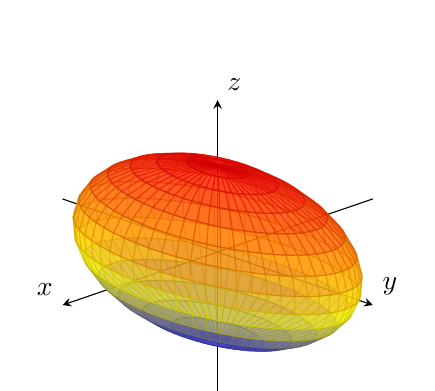
\begin{tikzpicture}[scale=1.15, baseline=(current bounding box.center)]
            \begin{axis}
            [view={135}{20},%colormap/blackwhite,
            axis lines=center, axis on top,ticks=none,
            set layers=default,axis equal,
            xlabel={$x$}, ylabel={$y$}, zlabel={$z$},
            xlabel style={anchor=south east},
            ylabel style={anchor=south west},
            zlabel style={anchor=south west},
            enlargelimits,
            tick align=inside,
            domain=0:2.00,
            samples=30, 
            z buffer=sort,
            ]
            \addplot3 [surf,opacity=0.4,domain=0:2*pi,
            domain y=0:360,on layer=axis foreground] ({sin(y)*sin(deg(x))},{2*cos(y)*sin(deg(x))},{cos(deg(x))});
            \end{axis}
        \end{tikzpicture}\\
    \midrule
    {$\frac{x^2}{a^2} + \frac{y^2}{b^2} - \frac{z^2}{c^2} = 1$} & {Enodelni eliptični hiperboloid} &
        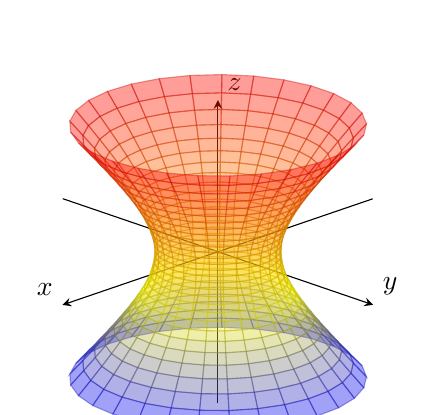
\begin{tikzpicture}[scale=1.15, baseline=(current bounding box.center)]
            \begin{axis}
            [view={135}{20},%colormap/blackwhite,
            axis lines=center, axis on top,ticks=none,
            set layers=default,axis equal,
            xlabel={$x$}, ylabel={$y$}, zlabel={$z$},
            xlabel style={anchor=south east},
            ylabel style={anchor=south west},
            zlabel style={anchor=south west},
            enlargelimits,
            tick align=inside,
            domain=0:2.00,
            samples=30, 
            z buffer=sort,
            ]
            \addplot3[surf,opacity=0.4,domain=0:360,y domain=-1.5:1.5,on layer=axis foreground]
                ({cosh(y)*cos(x)},{cosh(y)*sin(x)},{sinh(y)});
            \end{axis}
        \end{tikzpicture}\\
    \midrule
    {$\frac{x^2}{a^2} + \frac{y^2}{b^2} - \frac{z^2}{c^2} = 0$} & Eliptični stožec &
        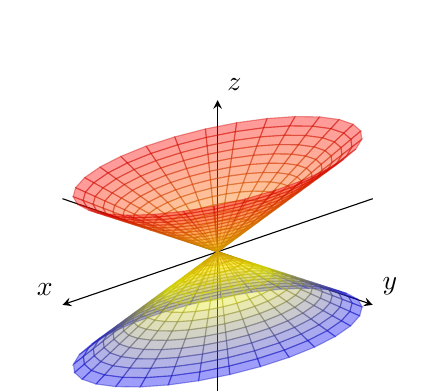
\begin{tikzpicture}[scale=1.15, baseline=(current bounding box.center)]
            \begin{axis}
            [view={135}{20},%colormap/blackwhite,
            axis lines=center, axis on top,ticks=none,
            set layers=default,axis equal,
            xlabel={$x$}, ylabel={$y$}, zlabel={$z$},
            xlabel style={anchor=south east},
            ylabel style={anchor=south west},
            zlabel style={anchor=south west},
            enlargelimits,
            tick align=inside,
            domain=0:2.00,
            samples=30, 
            z buffer=sort,
            ]
            \addplot3[surf,opacity=0.4,domain=0:2*pi,y domain=-1.5:1.5,on layer=axis foreground]
                ({2*y*cos(deg(x))},{y*sin(deg(x)},{y});
            \end{axis}
        \end{tikzpicture}\\
        \bottomrule
    \end{tabular}
\end{table}

\begin{table}[H]
    \centering
    \setcellgapes{15pt}
    \makegapedcells
    \begin{tabular}{ccc}
    \toprule
    {$\frac{x^2}{a^2} + \frac{y^2}{b^2} - \frac{z^2}{c^2} = -1$} & {Dvodelni eliptični hiperboloid} &
        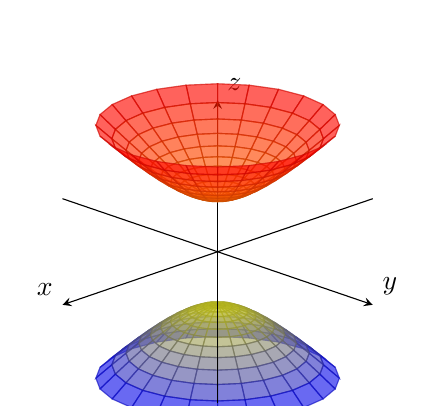
\begin{tikzpicture}[scale=1.15, baseline=(current bounding box.center)]
            \begin{axis}
            [view={135}{20},%colormap/blackwhite,
            axis lines=center, axis on top,ticks=none,
            set layers=default,axis equal,
            xlabel={$x$}, ylabel={$y$}, zlabel={$z$},
            xlabel style={anchor=south east},
            ylabel style={anchor=south west},
            zlabel style={anchor=south west},
            enlargelimits,
            tick align=inside,
            domain=0:2.00,
            samples=25, 
            z buffer=sort,
            ]
            \addplot3[surf,opacity=0.4,domain=0:360,y domain=-1.5:1.5,on layer=axis foreground]
                ({sinh(y)*cos(x)},{sinh(y)*sin(x)},{cosh(y)});
            \addplot3[surf,opacity=0.4,domain=0:360,y domain=-1.5:1.5]
                ({sinh(y)*cos(x)},{sinh(y)*sin(x)},{-cosh(y)});
        \end{axis}
    \end{tikzpicture}\\
    \midrule
    {$\frac{x^2}{a^2} + \frac{y^2}{b^2} = 1$} & {Eliptični valj} &
        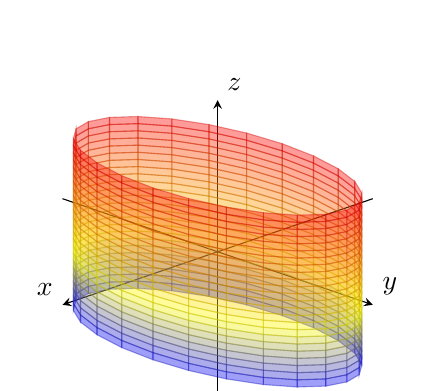
\begin{tikzpicture}[scale=1.15, baseline=(current bounding box.center)]
            \begin{axis}
            [view={135}{20},%colormap/blackwhite,
            axis lines=center, axis on top,ticks=none,
            set layers=default,axis equal,
            xlabel={$x$}, ylabel={$y$}, zlabel={$z$},
            xlabel style={anchor=south east},
            ylabel style={anchor=south west},
            zlabel style={anchor=south west},
            enlargelimits,
            tick align=inside,
            domain=0:2.00,
            samples=25, 
            z buffer=sort,
            ]
            \addplot3[surf,opacity=0.4,domain=0:360,y domain=-1:1,on layer=axis foreground]
                ({cos(x)},{2*sin(x)},y);
        \end{axis}
    \end{tikzpicture}\\
    \midrule
    {$\frac{x^2}{a^2} + \frac{y^2}{b^2} = z$} & {Eliptični paraboloid} &
        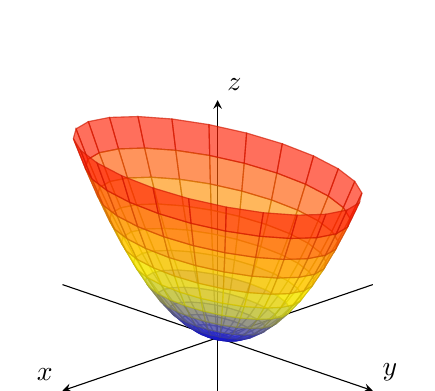
\begin{tikzpicture}[scale=1.15, baseline=(current bounding box.center)]
            \begin{axis}
            [view={135}{20},%colormap/blackwhite,
            axis lines=center, axis on top,ticks=none,
            set layers=default,axis equal,
            xlabel={$x$}, ylabel={$y$}, zlabel={$z$},
            xlabel style={anchor=south east},
            ylabel style={anchor=south west},
            zlabel style={anchor=south west},
            enlargelimits,
            tick align=inside,
            domain=0:2.00,
            samples=25, 
            z buffer=sort,
            ]
            \addplot3[surf,opacity=0.4,domain=0:360,y domain=-2:2,on layer=axis foreground]
                ({cos(x)*y},{2*sin(x)*y},y^2);
        \end{axis}
    \end{tikzpicture}\\
    \midrule
    {$\frac{x^2}{a^2} - \frac{y^2}{b^2} = \pm 1$} & {Hiperbolični valj} &
        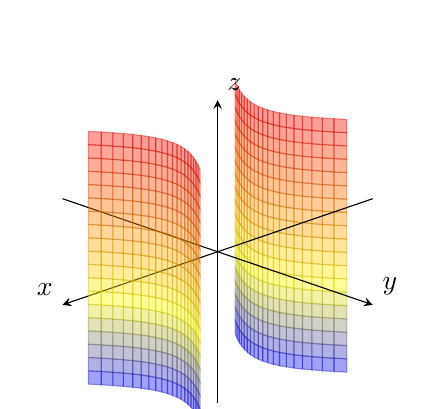
\begin{tikzpicture}[scale=1.15, baseline=(current bounding box.center)]
            \begin{axis}
            [view={135}{20},%colormap/blackwhite,
            axis lines=center, axis on top,ticks=none,
            set layers=default,axis equal,
            xlabel={$x$}, ylabel={$y$}, zlabel={$z$},
            xlabel style={anchor=south east},
            ylabel style={anchor=south west},
            zlabel style={anchor=south west},
            enlargelimits,
            tick align=inside,
            domain=0:2.00,
            samples=20, 
            z buffer=sort,
            ]
            \addplot3[surf,opacity=0.4,domain=-1:1,y domain=-2:2,on layer=axis foreground]
                ({cosh(x)},{sinh(x)},y);
            \addplot3[surf,opacity=0.4,domain=-1:1,y domain=-2:2]
                ({-cosh(x)},{sinh(x)},y);
        \end{axis}
    \end{tikzpicture}\\
    \midrule
    \end{tabular}
\end{table}

\begin{table}[H]
    \centering
    \setcellgapes{15pt}
    \makegapedcells
    \begin{tabular}{ccc}
        \toprule
        {$\frac{x^2}{a^2} - \frac{y^2}{b^2} = \pm z$} & {Hiperbolični paraboloid} &
        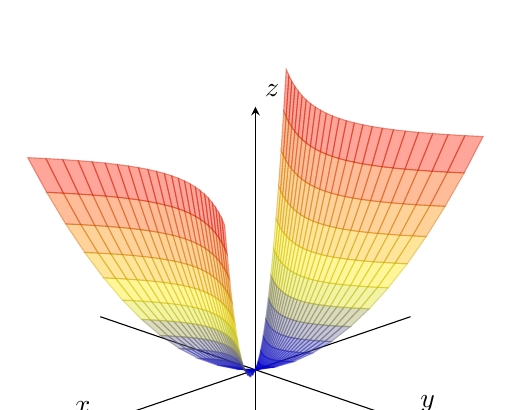
\begin{tikzpicture}[scale=1.15, baseline=(current bounding box.center)]
            \begin{axis}
            [view={135}{20},%colormap/blackwhite,
            axis lines=center, axis on top,ticks=none,
            set layers=default,axis equal,
            xlabel={$x$}, ylabel={$y$}, zlabel={$z$},
            xlabel style={anchor=south east},
            ylabel style={anchor=south west},
            zlabel style={anchor=south west},
            enlargelimits,
            tick align=inside,
            domain=0:2.00,
            samples=25, 
            z buffer=sort,
            ]
            \addplot3[surf,opacity=0.4,domain=-1:1,y domain=-2:2,on layer=axis foreground]
                ({cosh(x)*y},{sinh(x)*y},y^2);
            \end{axis}
        \end{tikzpicture}\\
        \midrule
        {$\frac{x^2}{a^2} = \pm y$} & {Parabolični valj} &
        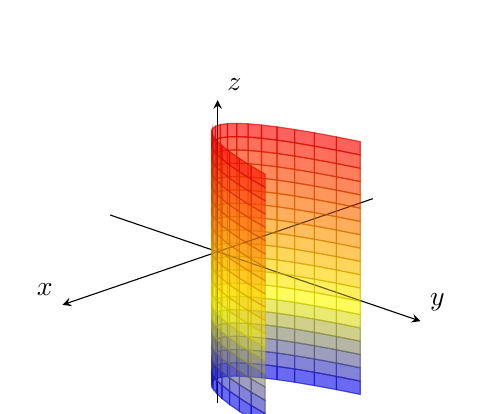
\begin{tikzpicture}[scale=1.15, baseline=(current bounding box.center)]
            \begin{axis}
            [view={135}{20},%colormap/blackwhite,
            axis lines=center, axis on top,ticks=none,
            set layers=default,axis equal,
            xlabel={$x$}, ylabel={$y$}, zlabel={$z$},
            xlabel style={anchor=south east},
            ylabel style={anchor=south west},
            zlabel style={anchor=south west},
            enlargelimits,
            tick align=inside,
            domain=0:2.00,
            samples=20, 
            z buffer=sort,
            ]
            \addplot3[surf,opacity=0.4,domain=-1:1,y domain=-2:2,on layer=axis foreground]
                (x,{2*x^2},-y);
            \addplot3[surf,opacity=0.4,domain=-1:1,y domain=-2:2]
                (-x,{2*x^2},-y);
        \end{axis}
        \end{tikzpicture}\\
        \midrule
    \end{tabular}
\end{table}

Za zgled navedimo še nekaj primerov uporabe teorije za določanje vrste ploskve.

\begin{zgled}
    Kadar ima matrika $A$ v kvadratni formi neničelne lastne vektorje, lahko hitro ugotovimo obliko ploskve s pomočjo lastnosti pozitivne definitnosti.
    Vzemimo enačbo $2x^2 + y^2 - 4xy - 4yz = 1$, ki ima matriko 
    $$A = \begin{bmatrix}
        2 & -2 & 0\\
        -2 & 1 & -2\\
        0 & -2 & 0
    \end{bmatrix}.$$
    Potem velja:
    \begin{itemize}
        \item $ \det A_1 = 2 > 0$
        \item $\displaystyle \det A_2 = \begin{vmatrix}
            2 & -2\\
            -2 & 1
        \end{vmatrix} = -2 < 0$
        \item $\displaystyle \det A = 2 \begin{vmatrix}
            2 & 0\\
            -2 & -2
        \end{vmatrix} = - 8 < 0$
    \end{itemize}
    Ker velja $\det A < 0$, so bodisi vse lastne vrednosti $A$ negativne bodisi je ena negativna in dve pozitivni.
    Če bi bile vse lastne vrednosti negativne, bi $A$ bila negativno definitna in bi veljalo tudi $\det A_1 < 0$ in $\det A_2 < 0$.
    Ker to ni res, ima $A$ eno negativno in dve pozitivni lastni vrednosti.
    Dana enačba torej predstavlja enodelni eliptični hiperboloid.
\end{zgled}

\begin{zgled}[Uporaba Sylvestrovega izreka in Lagrangeve metode]
    Vzemimo enačbo $3x^2 + 2y^2 + 3z^2 -2xy - 2yz - 2yz = 12.$ 
    Ta izraz lahko z Lagrangevo metodo napišemo kot kombinacijo kvadratov, in sicer $3(x - \frac{y}{3})^2 + \frac{5}{3} (y - \frac{3}{5}z)^2 + \frac{12}{5}z^2 = 12$.
    Sedaj imamo 
    \begin{equation*}
        D = \begin{bmatrix}
            3 & & \\
            & \frac{5}{3} & \\
            & & \frac{12}{5}
        \end{bmatrix}, \quad
        P \begin{bmatrix}
            x\\
            y\\
            z
        \end{bmatrix} = \begin{bmatrix}
            x - \frac{y}{3}\\
            y - \frac{3}{5}z\\
            z
        \end{bmatrix}, \quad 
        P = \begin{bmatrix}
            1 & -\frac{1}{3} & 0\\
            0 & 1 & -\frac{3}{5}\\
            0 & 0 & 1
        \end{bmatrix},
    \end{equation*}
    kjer je matrika $P$ obrnljiva. Sedaj imamo $\sprod{D P (x, y, z)}{P (x, y, z)} = 12$, kar je ekvivalentno $\sprod{P^\top D P (x, y, z)}{(x, y, z)} = 12$.
    Ker je $D$ kongruentna matriki identitete, je tudi $P^\top D P$ kongruentna matriki identitete.
    Zaradi enoličnosti so torej vse lastne vrednosti matrike $P^\top D P$ pozitivne in dana enačba predstavlja elipsoid.
\end{zgled}

\end{document}